
\part{Energy Mechanics}\label{part: energy mech}
\pagenumbering{arabic}
\begin{chapquote}{Joseph Fourier}
    ``Mathematics compares the most diverse phenomena and discovers the secret analogies that unite them.''
\end{chapquote}

\chapter*{Energy Mechanics Overview}

We may motivate our study of energy mechanics by asking a simple, yet profound question:
What is the fundamental nature of the universe?

If you lived in the time of Isaac Newton, the answer might be fairly simple - if we know the positions, velocities, and accelerations of objects, you can determine the future of that object with exacting certainty. 

Later, physicists would derive a different way of looking at mechanics -- using the methods of energy. This is what we explore in our study of variational calculus and energy mechanics. At the time, many physicists believed that this reframing was simply another expression of Newtonian physics. In some way, this is true. However, the energy method allows us to peer more deeply into the beating heart of physics to examine the fundamental qualities of nature. 

Examining the proceedings of physics in the 20th century, we see this become increasingly apparent. Mass -- Einstein had shown -- was fundamentally tied to the energy of particles in perhaps the most famous equation of all time, $E^2=m^2c^4+p^2c^2$. Later, as physicists began to develop quantum mechanics, energy, not forces, became the fundamental quantity to measure.

It is with this background that we motivate the study of energy mechanics. This subject gives us the key understanding needed to examine subjects from the smallest to the largest scales of the universe.

\chapter{Historical Background }

\color{red} Finish this section by improving some of the things with the brachistrochrone at the end.
\color{black}

In this chapter, I cover a brief history of the early years of energy mechanics. I will mostly cover the main figures and ideas that are instrumental to our study of energy mechanics. These main figures include Isaac Newton, Pierre de Fermat, and Johann Bernoulli.

The story of these figures is closely intertwined. It is impossible to discuss one figure without discussing the others as well. This section will thus take on a more chronological approach, but background information about some of the important characters is also included. Notably, I include some information about Isaac Newton for his far-reaching impacts in many aspects of mechanics.

The story of these figures will culminate in energy mechanics, possibly the most important implication of the studies of these historic figures. The foundations set by these scientists persist in the landscape of modern engineering and physics.

Euler, Lagrange, Hamilton, and others later contributions to the subjects will not be discussed here, but rather in \autoref{chap:calculus of variations}, \autoref{chap:lagrangian}, and \autoref{chap:hamiltonian}.

While the contributions of Weierstrass, Hilbert, and others is important to the mathematical solidification of the calculus of variations, I have chosen not to cover them in this text because I feel that it does not greatly aid readers in understanding the core of the subject.

The book by Goldstine \cite{goldstine_history_1980} has been especially useful in the development of this chapter. I highly recommend reading chapters 1-3 for readers who are interested in learning more about the history of this subject.

The goal of this chapter is not necessarily to derive many mathematical expressions, as most of the methods used were archaic and difficult to interpret for the modern reader. Goldstine has great historical analysis of these mathematics that is beyond the scope of the historical background presented here.

\section{Isaac Newton (1643-1727)} 

\begin{figure}[ht]
    \centering
    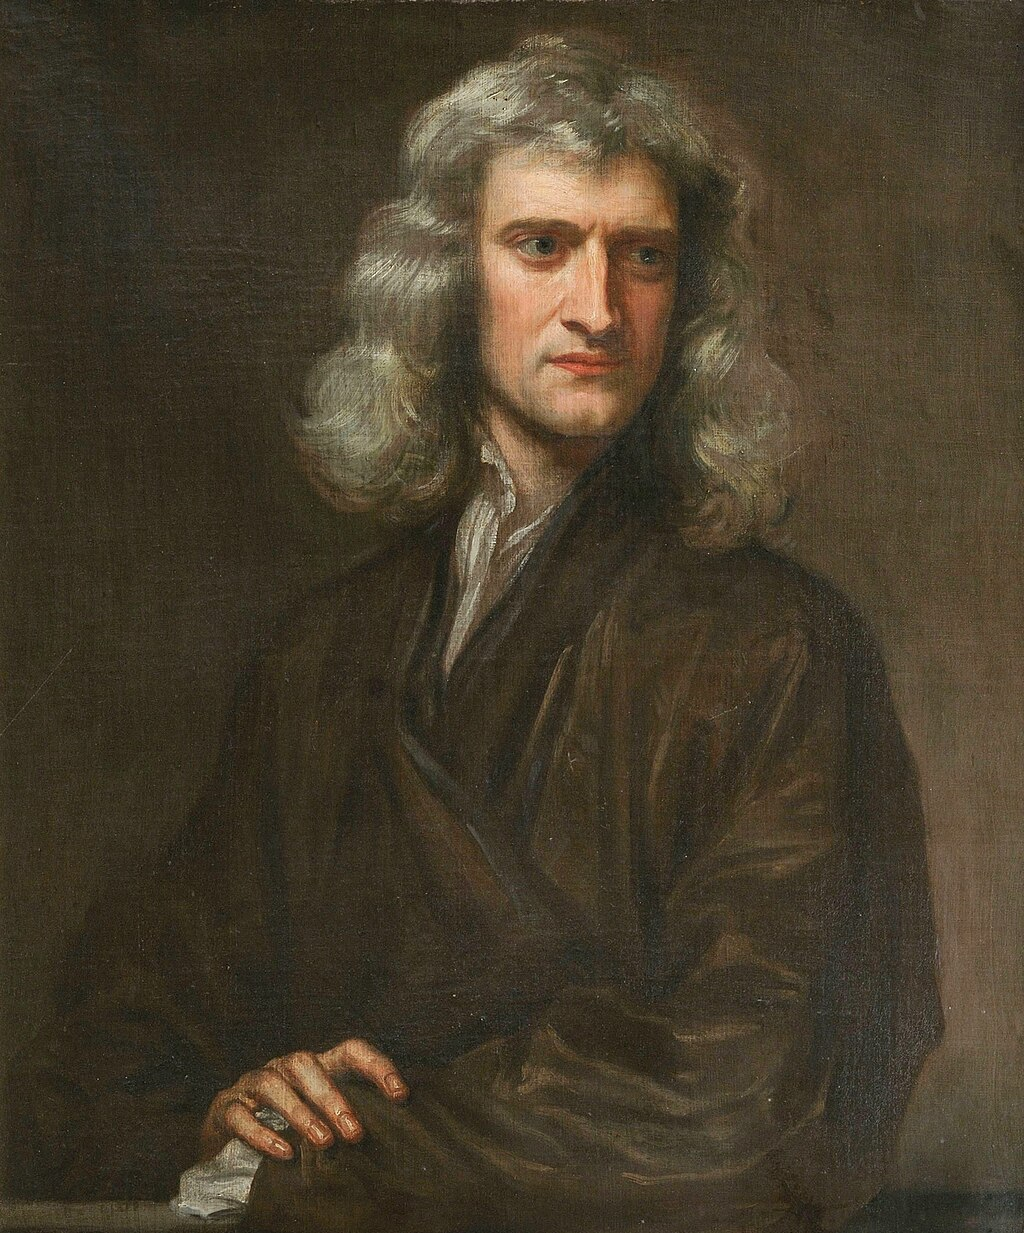
\includegraphics[width=0.5\linewidth]{Images/Portrait_of_Sir_Isaac_Newton,_1689_(brightened).jpg}
    \caption{Portrait of Sir Isaac Newton}
    \label{fig:Newton}
\end{figure}

The history of any kind of mechanics must start with a study of Isaac Newton. Newton is very famous for his description of mechanics based on forces and vectors. However, Newton is also instrumental character in our study of energy mechanics. 

In fact, Newton was instrumental to the development of Calculus of Variations, solving two of the first problems in the subject, the \textit{minimal resistance problem} and the \gls{brachistochrone} problem, which we will further explore in our study of the calculus of variations. It is on these subjects that we will spend most of the time.

Before we explore his contributions in this field, though, an understanding of his work in force-based mechanics and calculus is needed. This background section draws mostly from the text \cite{noauthor_isaac_2017}. Newton's work on variational calculus draws from several different sources, including the original \textit{Principia} and the \cite{goldstine_fermat_1980} chapter of Goldstine.

\subsection{Newton's Beginnings (1643-1661)}
In a story likely familiar to many people who find their interests in the realm of physics and engineering, Newton was born as an unwanted child to both his mother and father.

Born on Christmas Day in 1642 (Early January, 1643 in the modern calendar), Newton was born into an England in the midst of a civil war and full of strife. His father had died 3 months prior to his birth, and he was born prematurely. Newton was unwanted by his own mother, so he was raised by his maternal grandmother, Margery Ayscough.

Needless to say, Isaac Newton's early years were dominated by a lack of control and great turmoil. Thus, Newton took great solace in the isolation and fundamental truth of mathematics. This background in Newton's early life is likely to have had profound influences on his growth into adulthood and his later exploration of math.

Newton, in his years of study before college, had a great fascination for mechanical devices and an understanding of the world around him. It was in 1661 that he gained admittance to the Trinity College in Cambridge, right as the English Civil War was coming to a close.

\subsection{The Newtonian Calculus (1661-1679)}

During his time in college, Newton began his real exploration of mathematics. Newton's first great contribution to mathematics was in his studies of the Binomial theorem, which can give an expansion for a binomial raised to an arbitrary degree. Before Newton, there existed a theorem for the binomial theorem for the integers, $\mathbb{Z}$, which is presented below in \autoref{thm: binomial}.

\begin{theorem}[Binomial theorem]\label{thm: binomial}
    A binomial of form $x+y$ to a power n, where $n\in\mathbb{Z}$, the expansion can be written as:
    $$(x+y)^n=\sum_{k=0}^{n}\binom{n} {k}x^ky^{n-k}$$
    where $\binom{r}{k}$ is defined as:
    $$\binom{n}{k}=\frac{n!}{k!(n-k)!}$$
\end{theorem}

The original scope of this theorem only applies to the integer elements, $\mathbb{Z}$. Newton, however, extended the application of this theorem to the whole of the real numbers, $\mathbb{R}$. Newton's generalized theorem is then:


\begin{theorem}[Generalized Binomial theorem]
    A binomial of form $x+y$ to a power r, where $r\in\mathbb{R}$, the expansion can be written as:
    $$(x+y)^r=\sum_{k-0}^{\infty}\binom{r} {k}x^ry^{r-k}$$
    where $\binom{r}{k}$ is defined as:
    $$\binom{r}{k}=\frac{r(r-1)(r-2)\cdots(r-k+1)}{k!}$$
\end{theorem}

We note here that Newton has introduced an infinite sum! This is one of the first steps towards the methods of calculus. In fact, this equation has applicability towards the definition of the constant $e$, which is very fundemental in our studies of calculus. We can see this by inspection the definition of $e$ as:
$$ \lim_{x\to\infty} \left(1+\frac{1}{n}\right)^n$$
Using Newton's generalized binomial theorem, this infinite limit can be approximated and the value of $e$ can be closely approximated.

Newton continued his work on this subject, graduating in 1665. When Trinity University closed due to the Black Plague in the summer of that year, Newton took his work back home and began the most prolific part of his mathematical career, where he famously had the thought experiment of the apple falling towards the earth. It was during this time that Newton made his famous discoveries in optics and universal gravitation.

It was also during this period of great mathematical bounty that Newton began his studies of calculus. As early as 1665, Newton had methods to compute the derivative and find integral areas of curves. Using the generalized binomial theorem, Newton began to develop the concepts of integration and their applications to physics.

While the Newtonian methods of calculus are largely forgotten today in favor of the notation of Leibniz, it is without a doubt that Newton's contributions to the subject were extraordinary significant. Newton's contributions during this time will play a direct part in our later studies of energy mechanics.

\section{Fermat's Least Time Principle (1662)}
\begin{figure}[ht]
    \centering
    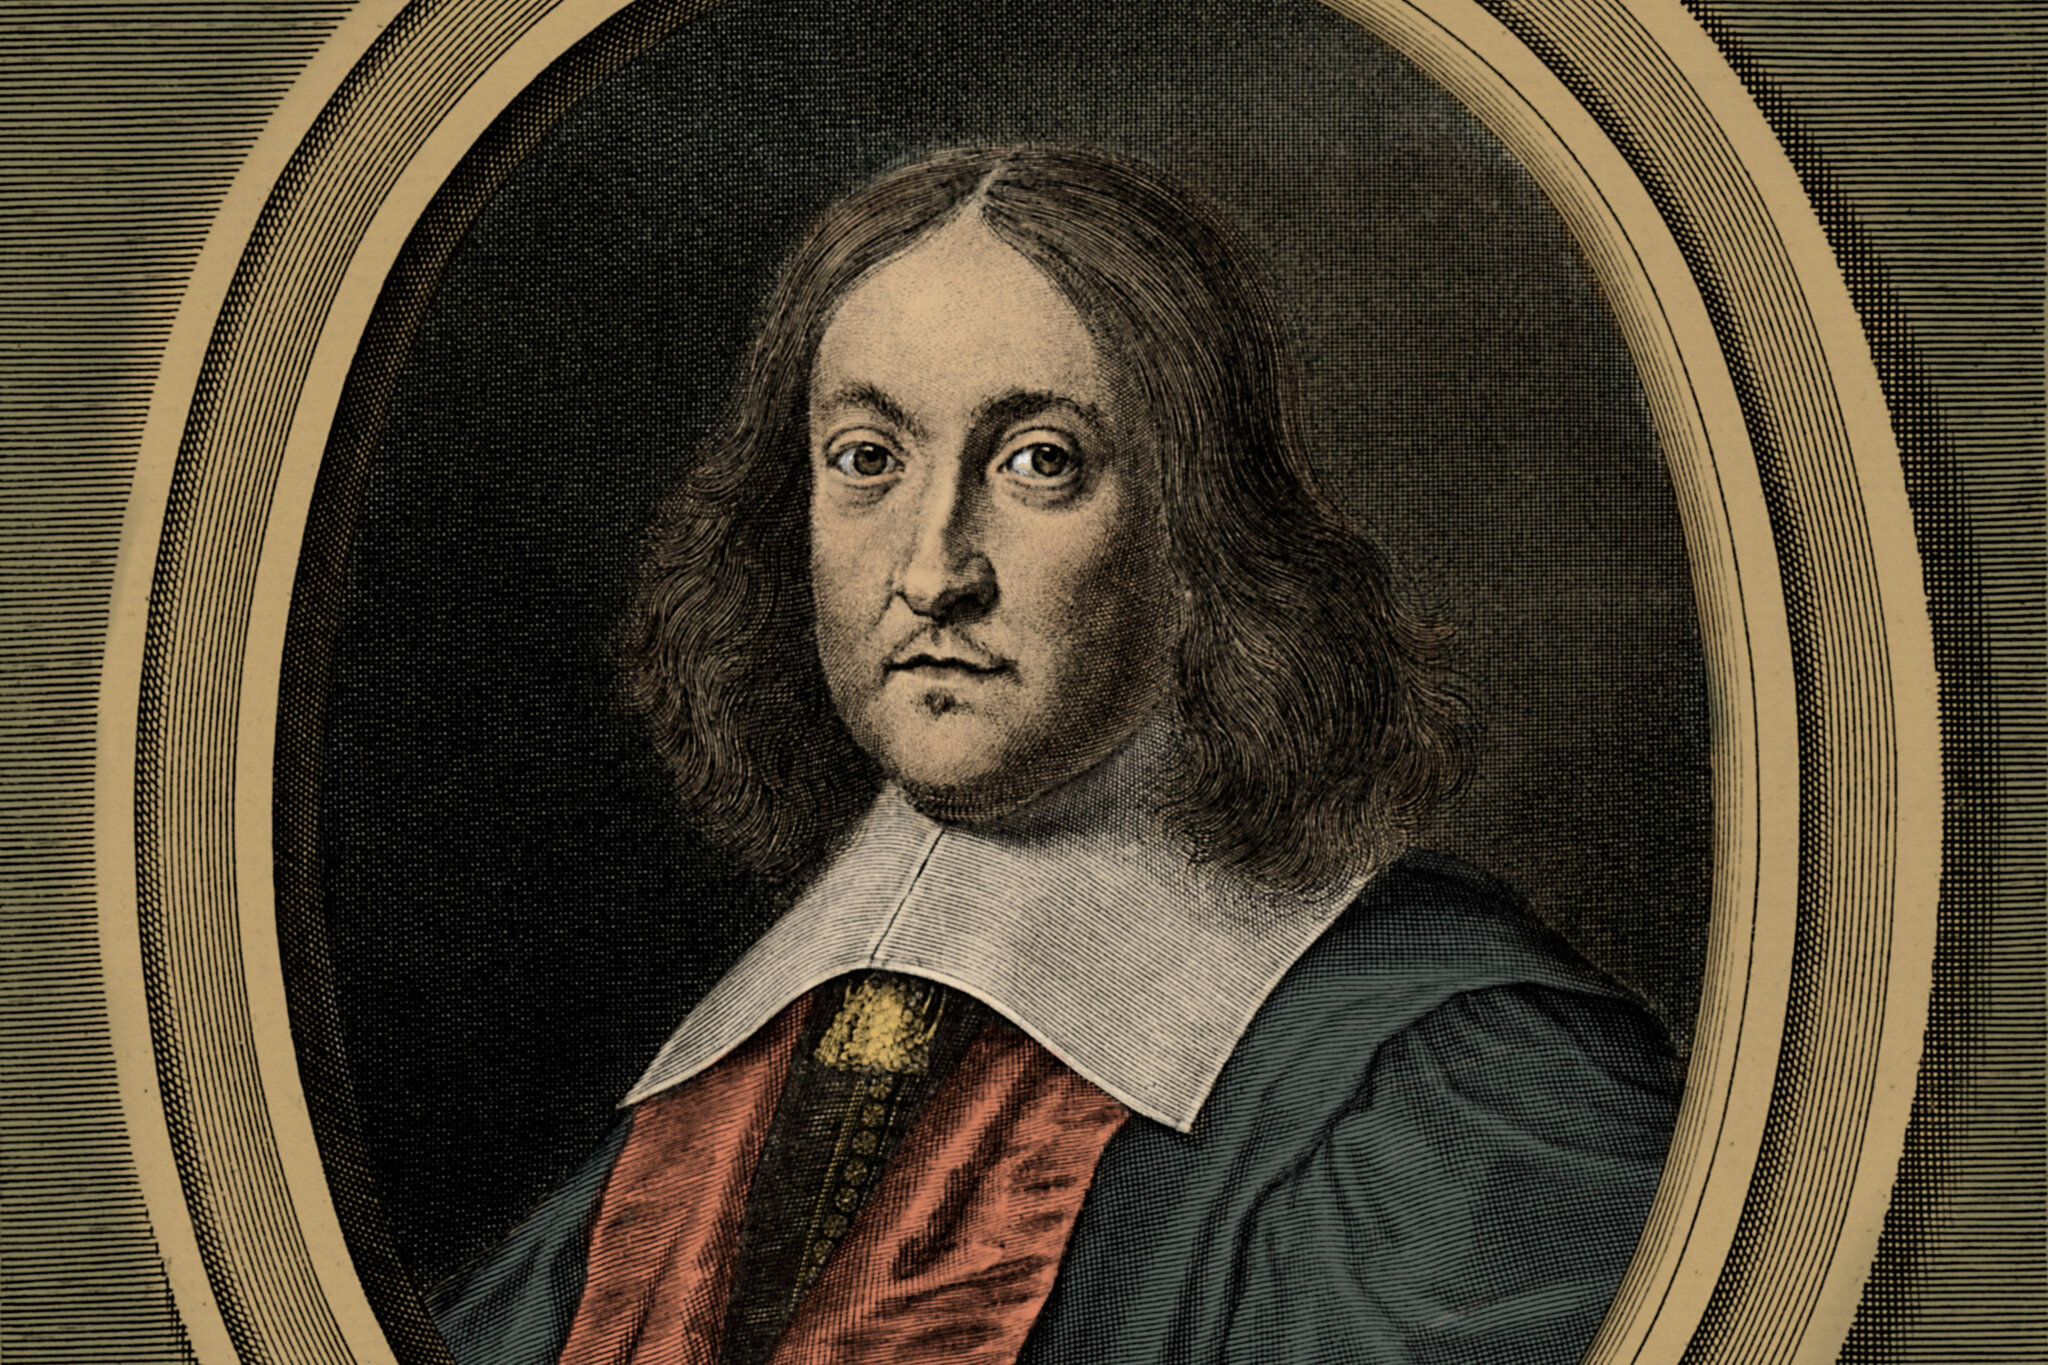
\includegraphics[width=0.75\linewidth]{Images/Fermat.jpg}
    \caption{A portrait of Pierre de Fermat}
    \label{fig:fermat}
\end{figure}
It is in the midst of Newton's most fruitful years that we must talk about Fermat's contributions to the subject of energy mechanics, which predate Newton's earliest contributions by nearly a score.

Fermat is famous in mathematics for \textit{Fermat's Last Theorem}, which remained unsolved for 358 years. A solution involving elliptic curves exists, which you can find an in-depth discussion in \cite{hellegouarch_invitation_2001} (this is entirely irrelevant to our work here). 

His contributions here, however, relate to the so-called \textit{Fermat's Principle of Least Time}. Fermat's biggest insight was the understanding that 'nature operates by means and ways that are easiest and fastest'. Although this way seem a simple statement, it will underlie the physical principle at the root of energy mechanics.

Fermat's Principle of Least Time involves finding a light path such that the time is minimized.\endnote{It can be shown that this is not exactly true, as the only condition required for sufficiency in this problem is that the changes to the variation are of the second-order. Fermat's condition is simply one such case of this. See \cite{feynman_feynman_1963} for more info.}Fermat's set up is as shown in \autoref{fig:least time ray}. Fermat noticed that the light path will refract and change its angle when moving through a medium where the speed of light is slower.

The law of reflection can also be shown from Fermat's Principle, although that will not be done here. It is quite similar to the derivation of the refraction law. If you find an interest in the subject matter here, a much more in-depth discussion in the wonderful Feynman lectures on physics can be found in \cite{feynman_feynman_1963}.

\begin{figure}
    \centering
    

\tikzset{every picture/.style={line width=0.75pt}} %set default line width to 0.75pt        

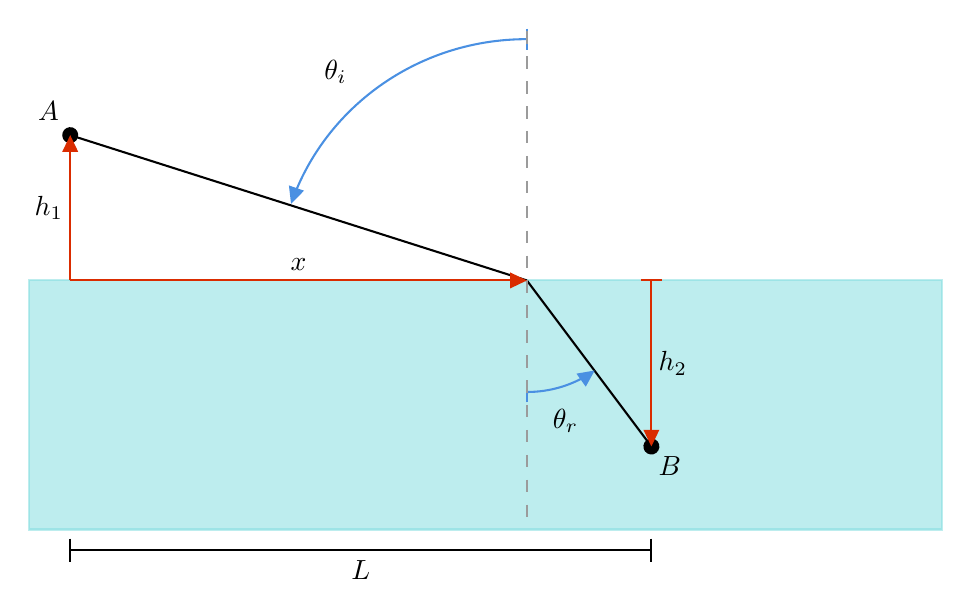
\begin{tikzpicture}[x=0.75pt,y=0.75pt,yscale=-1,xscale=1]
%uncomment if require: \path (0,300); %set diagram left start at 0, and has height of 300

%Shape: Rectangle [id:dp8879936647316232] 
\draw  [color={rgb, 255:red, 126; green, 219; blue, 222 }  ,draw opacity=0.51 ][fill={rgb, 255:red, 126; green, 219; blue, 222 }  ,fill opacity=0.51 ] (110,130) -- (550,130) -- (550,250) -- (110,250) -- cycle ;
%Straight Lines [id:da9092976870956871] 
\draw    (130,60) -- (350,130) ;
\draw [shift={(130,60)}, rotate = 17.65] [color={rgb, 255:red, 0; green, 0; blue, 0 }  ][fill={rgb, 255:red, 0; green, 0; blue, 0 }  ][line width=0.75]      (0, 0) circle [x radius= 3.35, y radius= 3.35]   ;
%Straight Lines [id:da28057638271133667] 
\draw    (350,130) -- (410,210) ;
\draw [shift={(410,210)}, rotate = 53.13] [color={rgb, 255:red, 0; green, 0; blue, 0 }  ][fill={rgb, 255:red, 0; green, 0; blue, 0 }  ][line width=0.75]      (0, 0) circle [x radius= 3.35, y radius= 3.35]   ;
%Shape: Arc [id:dp9634726814563676] 
\draw  [draw opacity=0] (236.39,93.09) .. controls (252.29,46.98) and (297.15,13.75) .. (350,13.75) -- (350,130) -- cycle ; \draw [color={rgb, 255:red, 74; green, 144; blue, 226 }  ,draw opacity=1 ]   (237.64,89.65) .. controls (254.54,45.34) and (298.47,13.75) .. (350,13.75) ; \draw [shift={(350,13.75)}, rotate = 180] [color={rgb, 255:red, 74; green, 144; blue, 226 }  ,draw opacity=1 ][line width=0.75]    (0,5.03) -- (0,-5.03)   ; \draw [shift={(236.39,93.09)}, rotate = 289.02] [fill={rgb, 255:red, 74; green, 144; blue, 226 }  ,fill opacity=1 ][line width=0.08]  [draw opacity=0] (8.04,-3.86) -- (0,0) -- (8.04,3.86) -- cycle    ;
%Shape: Arc [id:dp3411757437853058] 
\draw  [draw opacity=0] (382.69,173.39) .. controls (373.53,179.9) and (362.23,183.75) .. (350,183.75) -- (350,130) -- cycle ; \draw [color={rgb, 255:red, 74; green, 144; blue, 226 }  ,draw opacity=1 ]   (380.17,175.08) .. controls (371.49,180.56) and (361.13,183.75) .. (350,183.75) ; \draw [shift={(350,183.75)}, rotate = 360] [color={rgb, 255:red, 74; green, 144; blue, 226 }  ,draw opacity=1 ][line width=0.75]    (0,5.03) -- (0,-5.03)   ; \draw [shift={(382.69,173.39)}, rotate = 144.58] [fill={rgb, 255:red, 74; green, 144; blue, 226 }  ,fill opacity=1 ][line width=0.08]  [draw opacity=0] (8.04,-3.86) -- (0,0) -- (8.04,3.86) -- cycle    ;
%Straight Lines [id:da9977458453758269] 
\draw [color={rgb, 255:red, 155; green, 155; blue, 155 }  ,draw opacity=1 ] [dash pattern={on 4.5pt off 4.5pt}]  (350,10) -- (350,250) ;
%Straight Lines [id:da33608457803837766] 
\draw    (130,260) -- (410,260) ;
\draw [shift={(410,260)}, rotate = 180] [color={rgb, 255:red, 0; green, 0; blue, 0 }  ][line width=0.75]    (0,5.59) -- (0,-5.59)   ;
\draw [shift={(130,260)}, rotate = 180] [color={rgb, 255:red, 0; green, 0; blue, 0 }  ][line width=0.75]    (0,5.59) -- (0,-5.59)   ;
%Straight Lines [id:da7724749653392198] 
\draw [color={rgb, 255:red, 218; green, 44; blue, 0 }  ,draw opacity=1 ]   (410,130) -- (410,207) ;
\draw [shift={(410,210)}, rotate = 270] [fill={rgb, 255:red, 218; green, 44; blue, 0 }  ,fill opacity=1 ][line width=0.08]  [draw opacity=0] (8.04,-3.86) -- (0,0) -- (8.04,3.86) -- cycle    ;
\draw [shift={(410,130)}, rotate = 270] [color={rgb, 255:red, 218; green, 44; blue, 0 }  ,draw opacity=1 ][line width=0.75]    (0,5.03) -- (0,-5.03)   ;
%Straight Lines [id:da7478103517482707] 
\draw [color={rgb, 255:red, 218; green, 44; blue, 0 }  ,draw opacity=1 ]   (130,130) -- (130,63) ;
\draw [shift={(130,60)}, rotate = 90] [fill={rgb, 255:red, 218; green, 44; blue, 0 }  ,fill opacity=1 ][line width=0.08]  [draw opacity=0] (8.04,-3.86) -- (0,0) -- (8.04,3.86) -- cycle    ;
%Straight Lines [id:da3656630452978258] 
\draw [color={rgb, 255:red, 218; green, 44; blue, 0 }  ,draw opacity=1 ]   (130,130) -- (347,130) ;
\draw [shift={(350,130)}, rotate = 180] [fill={rgb, 255:red, 218; green, 44; blue, 0 }  ,fill opacity=1 ][line width=0.08]  [draw opacity=0] (8.04,-3.86) -- (0,0) -- (8.04,3.86) -- cycle    ;

% Text Node
\draw (251,22.4) node [anchor=north west][inner sep=0.75pt]    {$\theta _{i}$};
% Text Node
\draw (361,190.4) node [anchor=north west][inner sep=0.75pt]    {$\theta _{r}$};
% Text Node
\draw (270,263.4) node [anchor=north] [inner sep=0.75pt]    {$L$};
% Text Node
\draw (412,170) node [anchor=west] [inner sep=0.75pt]    {$h_{2}$};
% Text Node
\draw (128,95) node [anchor=east] [inner sep=0.75pt]    {$h_{1}$};
% Text Node
\draw (126,54.6) node [anchor=south east] [inner sep=0.75pt]    {$A$};
% Text Node
\draw (412,213.4) node [anchor=north west][inner sep=0.75pt]    {$B$};
% Text Node
\draw (240,126.6) node [anchor=south] [inner sep=0.75pt]    {$x$};

\end{tikzpicture}


    \caption{Fermat's Set-up for the Least Time Problem for a Light Ray}
    \label{fig:least time ray}
\end{figure}

I do not delve into the proof by Fermat, since it uses archaic methods of calculus that are more confusing than enlightening to the modern audience. Fermat's solution is mostly geometric and it involves a geometric proof using the Law of Cosines. 

Instead, I will take a more modern approach which follows roughly along with Fermat. Following the standard procedures of calculus, we will find a minimization of the function by considering the point where the first derivative is zero.

I will present here a modern derivation of this principle, because I believe it makes the later derivations more satisfying and provides a brief introduction to the methodologies of the calculus of variations.

Starting from the set-up shown in \autoref{fig:least time ray}, we can write equations for the time for each of the sections of the light path. To do so, we use the fundemental relationship for velocity:
$$t=\frac{d}{v}$$
Using the definition that the velocity in an optical medium is $v=\frac{c}{n}$, we can write the time for each section. Starting with the section in the lower optical density:
$$t_{upper}=\frac{n_i\sqrt{{h_1}^2+x^2}}{c}$$
And for the more dense optical surface, we do the same:
$$t_{lower}=\frac{n_r\sqrt{{h_2}^2+(l-x)^2}}{c}$$
Altogether, we have a the following relationship:
$$t=\frac{n_i\sqrt{{h_1}^2+x^2}}{c}+\frac{n_r\sqrt{{h_2}^2+(l-x)^2}}{c}$$
We can achieve the desired goal of finding the minimum time by taking the derivative of this time with respect to the variable $x$ and setting it equal to zero as follows:
$$\frac{dt}{dx}=\frac{n_ix}{c\sqrt{{h_1}^2+x^2}}-\frac{n_r(l-x)}{c\sqrt{{h_2}^2+(l-x)^2}}=0$$
A rearrangement leads to the following:
$$\frac{n_ix}{c\sqrt{{h_1}^2+x^2}}=\frac{n_r(l-x)}{c\sqrt{{h_2}^2+(l-x)^2}}$$
Using the established angles $\theta_1$ and $\theta_2$, we can express this relation more simply as:
\begin{gather}
    \color{blue}\boxed{\color{black}n_i\sin\theta_i=n_r\sin\theta_r}\\
    \color{blue}\mathrm{Snell's \ Law}
\end{gather}
We will keep this result in mind, as we will see it again when we solve the problem of the \gls{brachistochrone}.

\subsection{Connection to Quantum Electrodynamics}\label{sec: connection to quantum}
The curious reader may not be fully satisfied with the answer given by Fermat. Why does light take a path that minimizes time? Is there any physical reason for this? In this section we will take a brief aside from the history to answer these questions.

To fully understand this question, we must understand that during Fermat's time there was a rift in the world of physics concerning the behavior of light. Some, such as Newton, believed light to be a particle. Others, led by the prominent dutch mathematician Christaan Huygens, believed that light was a wave.

When we consider light to be a wave, the problem of least time is solved! If the light takes a suboptimal trajectory (that is, a trajectory that takes more time), the wave will destructively interfere with itself. It is only light which takes the shortest path which will constructively interfere and produce a  bright spot! So the riddle is solved. Newton is wrong, and light is in fact a wave! The problem is this: We can measure individual packets of light, photons, arriving at photomultipliers or digital sensors. When a light source gets dimmer, we simply measure fewer numbers of photons, but the energies associated with each one is exactly the same.

So we must again reconsider our viewpoint. Light must showcase both properties to match all of the evidence! Of course, it is now popularly understood that light - and in fact everything else - exhibits both properties in a wave-particle duality.

The existence of this duality alone does not necessarily answer our question, but it gets us on the path to doing so. The true answer to this question remained unknown for nearly 300 years -- until the advent of \gls{qed} in the 1940's, the invention of which would lead Richard Feynman to winning the Nobel Prize in physics.

Of course, explaining a Nobel Prize worthy achievement in physics is no easy task! Luckily, Feynman himself has offered quite a simple explanation of the phenomena of light in his book, \cite{richard_phillips_feynman_qed_1988}. I highly suggest the interested reader to read this book in full (it is quite short and easy to read) to better comprehend this section. Here, I will present only a portion of Feynman's argument to convince you that the least action principle naturally arises from \gls{qed}.

\subsubsection{Mirrors}
Although we earlier made a computation for Snell's Law using Fermat's principle, we will instead take the case of the mirror here. The derivation of the equivalent least time principle for the mirror is left as an exercise, but follows from a similar procedure.
\begin{exercise}
    Using the same methods as were used to derive Snell's Law, find the criteria that minimizes time for the case of a mirror, which reflects light instead of refracting it. The set up for such a mirror system is shown in \autoref{fig:mirror}.
\begin{figure}[H]
    \centering


\tikzset{every picture/.style={line width=0.75pt}} %set default line width to 0.75pt        

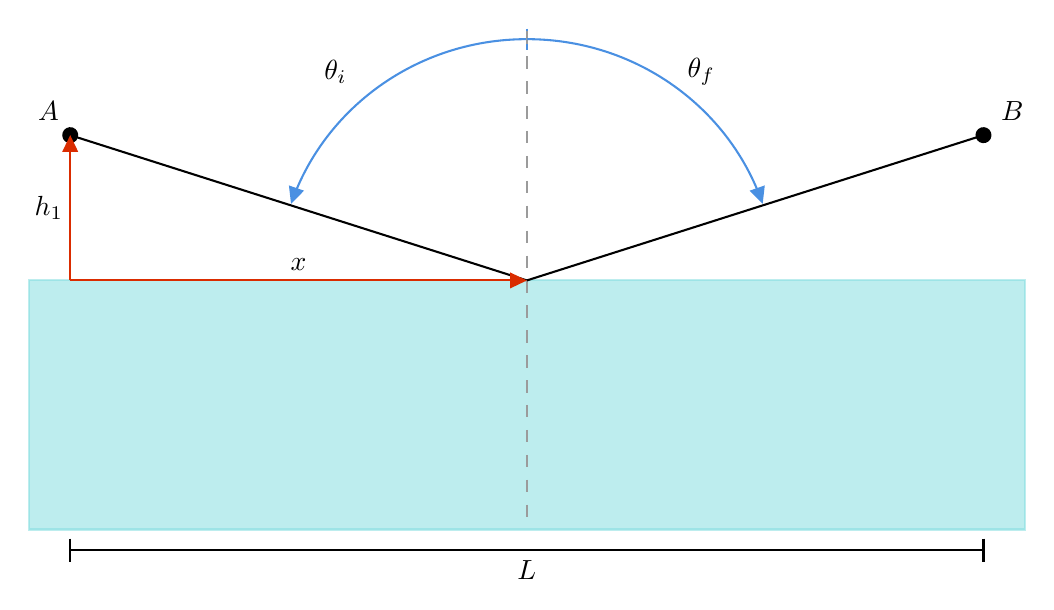
\begin{tikzpicture}[x=0.75pt,y=0.75pt,yscale=-1,xscale=1]
%uncomment if require: \path (0,300); %set diagram left start at 0, and has height of 300

%Shape: Rectangle [id:dp6275989944924254] 
\draw  [color={rgb, 255:red, 126; green, 219; blue, 222 }  ,draw opacity=0.51 ][fill={rgb, 255:red, 126; green, 219; blue, 222 }  ,fill opacity=0.51 ] (90,140) -- (570,140) -- (570,260) -- (90,260) -- cycle ;
%Straight Lines [id:da6083348703679279] 
\draw    (110,70) -- (330,140) ;
\draw [shift={(110,70)}, rotate = 17.65] [color={rgb, 255:red, 0; green, 0; blue, 0 }  ][fill={rgb, 255:red, 0; green, 0; blue, 0 }  ][line width=0.75]      (0, 0) circle [x radius= 3.35, y radius= 3.35]   ;
%Shape: Arc [id:dp6990536523303199] 
\draw  [draw opacity=0] (216.39,103.09) .. controls (232.29,56.98) and (277.15,23.75) .. (330,23.75) -- (330,140) -- cycle ; \draw [color={rgb, 255:red, 74; green, 144; blue, 226 }  ,draw opacity=1 ]   (217.64,99.65) .. controls (234.54,55.34) and (278.47,23.75) .. (330,23.75) ; \draw [shift={(330,23.75)}, rotate = 180] [color={rgb, 255:red, 74; green, 144; blue, 226 }  ,draw opacity=1 ][line width=0.75]    (0,5.03) -- (0,-5.03)   ; \draw [shift={(216.39,103.09)}, rotate = 289.02] [fill={rgb, 255:red, 74; green, 144; blue, 226 }  ,fill opacity=1 ][line width=0.08]  [draw opacity=0] (8.04,-3.86) -- (0,0) -- (8.04,3.86) -- cycle    ;
%Straight Lines [id:da21803443744202755] 
\draw [color={rgb, 255:red, 155; green, 155; blue, 155 }  ,draw opacity=1 ] [dash pattern={on 4.5pt off 4.5pt}]  (330,20) -- (330,260) ;
%Straight Lines [id:da33439071823558864] 
\draw    (110,270) -- (550,270) ;
\draw [shift={(550,270)}, rotate = 180] [color={rgb, 255:red, 0; green, 0; blue, 0 }  ][line width=0.75]    (0,5.59) -- (0,-5.59)   ;
\draw [shift={(110,270)}, rotate = 180] [color={rgb, 255:red, 0; green, 0; blue, 0 }  ][line width=0.75]    (0,5.59) -- (0,-5.59)   ;
%Straight Lines [id:da48893176676953176] 
\draw [color={rgb, 255:red, 218; green, 44; blue, 0 }  ,draw opacity=1 ]   (110,140) -- (110,73) ;
\draw [shift={(110,70)}, rotate = 90] [fill={rgb, 255:red, 218; green, 44; blue, 0 }  ,fill opacity=1 ][line width=0.08]  [draw opacity=0] (8.04,-3.86) -- (0,0) -- (8.04,3.86) -- cycle    ;
%Straight Lines [id:da28787272817377096] 
\draw [color={rgb, 255:red, 218; green, 44; blue, 0 }  ,draw opacity=1 ]   (110,140) -- (327,140) ;
\draw [shift={(330,140)}, rotate = 180] [fill={rgb, 255:red, 218; green, 44; blue, 0 }  ,fill opacity=1 ][line width=0.08]  [draw opacity=0] (8.04,-3.86) -- (0,0) -- (8.04,3.86) -- cycle    ;
%Straight Lines [id:da5717809459497747] 
\draw    (550,70) -- (330,140) ;
\draw [shift={(550,70)}, rotate = 162.35] [color={rgb, 255:red, 0; green, 0; blue, 0 }  ][fill={rgb, 255:red, 0; green, 0; blue, 0 }  ][line width=0.75]      (0, 0) circle [x radius= 3.35, y radius= 3.35]   ;
%Shape: Arc [id:dp08924222560062933] 
\draw  [draw opacity=0] (330,23.75) .. controls (330,23.75) and (330,23.75) .. (330,23.75) .. controls (382.85,23.75) and (427.71,56.98) .. (443.61,103.09) -- (330,140) -- cycle ; \draw [color={rgb, 255:red, 74; green, 144; blue, 226 }  ,draw opacity=1 ]   (330,23.75) .. controls (381.8,23.75) and (425.91,55.66) .. (442.62,100.34) ; \draw [shift={(443.61,103.09)}, rotate = 250.98] [fill={rgb, 255:red, 74; green, 144; blue, 226 }  ,fill opacity=1 ][line width=0.08]  [draw opacity=0] (8.04,-3.86) -- (0,0) -- (8.04,3.86) -- cycle    ; 

% Text Node
\draw (231,32.4) node [anchor=north west][inner sep=0.75pt]    {$\theta _{i}$};
% Text Node
\draw (330,273.4) node [anchor=north] [inner sep=0.75pt]    {$L$};
% Text Node
\draw (108,105) node [anchor=east] [inner sep=0.75pt]    {$h_{1}$};
% Text Node
\draw (106,64.6) node [anchor=south east] [inner sep=0.75pt]    {$A$};
% Text Node
\draw (557,52.4) node [anchor=north west][inner sep=0.75pt]    {$B$};
% Text Node
\draw (220,136.6) node [anchor=south] [inner sep=0.75pt]    {$x$};
% Text Node
\draw (406,31.4) node [anchor=north west][inner sep=0.75pt]    {$\theta _{f}$};


\end{tikzpicture}

    \caption{Mirror Set-Up}
    \label{fig:mirror}
\end{figure}
\end{exercise}

Readers who carefully perform the derivation above using the methods shown before will find that in the case of the mirror, $\theta_i=\theta_f$. That is, the incident angle is equal to the outgoing angle. In our previous derivations, we showed this to be a consequence of the principle of least time.

If we think of the problem more `democratically', we shouldn't give any preference to any one path though! Let's consider all of the straight line paths that light can take. A few of these paths are shown in \autoref{fig:light traj}.
\begin{figure}[ht]
    \centering

% Pattern Info
 
\tikzset{
pattern size/.store in=\mcSize, 
pattern size = 5pt,
pattern thickness/.store in=\mcThickness, 
pattern thickness = 0.3pt,
pattern radius/.store in=\mcRadius, 
pattern radius = 1pt}
\makeatletter
\pgfutil@ifundefined{pgf@pattern@name@_6b3jznvkh}{
\pgfdeclarepatternformonly[\mcThickness,\mcSize]{_6b3jznvkh}
{\pgfqpoint{0pt}{0pt}}
{\pgfpoint{\mcSize+\mcThickness}{\mcSize+\mcThickness}}
{\pgfpoint{\mcSize}{\mcSize}}
{
\pgfsetcolor{\tikz@pattern@color}
\pgfsetlinewidth{\mcThickness}
\pgfpathmoveto{\pgfqpoint{0pt}{0pt}}
\pgfpathlineto{\pgfpoint{\mcSize+\mcThickness}{\mcSize+\mcThickness}}
\pgfusepath{stroke}
}}
\makeatother
\tikzset{every picture/.style={line width=0.75pt}} %set default line width to 0.75pt        

\begin{tikzpicture}[x=0.75pt,y=0.75pt,yscale=-1,xscale=1]
%uncomment if require: \path (0,300); %set diagram left start at 0, and has height of 300

%Shape: Rectangle [id:dp13216032235189357] 
\draw  [color={rgb, 255:red, 126; green, 219; blue, 222 }  ,draw opacity=0.51 ][fill={rgb, 255:red, 126; green, 219; blue, 222 }  ,fill opacity=0.51 ] (100,240) -- (560,240) -- (560,280) -- (100,280) -- cycle ;
%Shape: Rectangle [id:dp7152402004015799] 
\draw  [pattern=_6b3jznvkh,pattern size=7.5pt,pattern thickness=0.75pt,pattern radius=0pt, pattern color={rgb, 255:red, 0; green, 0; blue, 0}] (320,130) -- (340,130) -- (340,170) -- (320,170) -- cycle ;
%Straight Lines [id:da14645204907035414] 
\draw [line width=0.75]    (140,160) -- (330,240) ;
%Straight Lines [id:da5333244615267384] 
\draw [line width=0.75]    (520,160) -- (330,240) ;
%Straight Lines [id:da19778015344004796] 
\draw [line width=0.75]    (140,160) -- (240,240) ;
%Straight Lines [id:da47608518269163747] 
\draw [line width=0.75]    (520,160) -- (240,240) ;
%Straight Lines [id:da14756293959452693] 
\draw [line width=0.75]    (520,160) -- (420,240) ;
%Straight Lines [id:da7018685323723184] 
\draw [line width=0.75]    (140,160) -- (420,240) ;
%Straight Lines [id:da7703911392020962] 
\draw [line width=0.75]    (140,160) -- (180,240) ;
%Straight Lines [id:da3928605678682944] 
\draw [line width=0.75]    (520,160) -- (180,240) ;
%Straight Lines [id:da5605057304874714] 
\draw [line width=0.75]    (520,160) -- (480,240) ;
%Straight Lines [id:da19372382419577583] 
\draw [line width=0.75]    (140,160) -- (480,240) ;

% Text Node
\draw (121,142.4) node [anchor=north west][inner sep=0.75pt]    {$A$};
% Text Node
\draw (527,142.4) node [anchor=north west][inner sep=0.75pt]    {$B$};


\end{tikzpicture}
    \caption{Possible trajectories of light across a mirror}
    \label{fig:light traj}
\end{figure}

Of course, we know from experience that mirrors do not show reflections like this. If they did, we could look from point $A$ at any angle and we would see $B$ centered in the view. There must be something wrong with our model! And there is: we are missing a key component called the phase of the light. Essentially, the phase measures the `direction' of the light (this description will suffice for our purposes). We can think of the phase of the light as a little clock that moves with the light. The clock hand starts pointing straight up at point $A$, and it winds around at a constant rate until the photon reaches point $B$, at that point, we measure the direction the clock hand is pointing. This direction will be a vector with a length of 1, but the direction will change based on the time duration!

So, if we take phase into consideration, we get a new picture of the phenomenon, which is shown in \autoref{fig:polarization paths}. What is shown is the time that it takes each ray of light to reach point $B$ based on the point where it hits the mirror. These are marked with a red marker below the point of intersection with the mirror.

\begin{figure}[ht]
    \centering



% Pattern Info
 
\tikzset{
pattern size/.store in=\mcSize, 
pattern size = 5pt,
pattern thickness/.store in=\mcThickness, 
pattern thickness = 0.3pt,
pattern radius/.store in=\mcRadius, 
pattern radius = 1pt}
\makeatletter
\pgfutil@ifundefined{pgf@pattern@name@_bnexa4sr6}{
\pgfdeclarepatternformonly[\mcThickness,\mcSize]{_bnexa4sr6}
{\pgfqpoint{0pt}{0pt}}
{\pgfpoint{\mcSize+\mcThickness}{\mcSize+\mcThickness}}
{\pgfpoint{\mcSize}{\mcSize}}
{
\pgfsetcolor{\tikz@pattern@color}
\pgfsetlinewidth{\mcThickness}
\pgfpathmoveto{\pgfqpoint{0pt}{0pt}}
\pgfpathlineto{\pgfpoint{\mcSize+\mcThickness}{\mcSize+\mcThickness}}
\pgfusepath{stroke}
}}
\makeatother
\tikzset{every picture/.style={line width=0.75pt}} %set default line width to 0.75pt        

\begin{tikzpicture}[x=0.75pt,y=0.75pt,yscale=-1,xscale=1]
%uncomment if require: \path (0,415); %set diagram left start at 0, and has height of 415

%Shape: Rectangle [id:dp13216032235189357] 
\draw  [color={rgb, 255:red, 126; green, 219; blue, 222 }  ,draw opacity=0.51 ][fill={rgb, 255:red, 126; green, 219; blue, 222 }  ,fill opacity=0.51 ] (100,130) -- (560,130) -- (560,170) -- (100,170) -- cycle ;
%Shape: Rectangle [id:dp7152402004015799] 
\draw  [pattern=_bnexa4sr6,pattern size=7.5pt,pattern thickness=0.75pt,pattern radius=0pt, pattern color={rgb, 255:red, 0; green, 0; blue, 0}] (320,20) -- (340,20) -- (340,60) -- (320,60) -- cycle ;
%Straight Lines [id:da14645204907035414] 
\draw [line width=0.75]    (140,50) -- (330,130) ;
%Straight Lines [id:da5333244615267384] 
\draw [line width=0.75]    (520,50) -- (330,130) ;
%Straight Lines [id:da19778015344004796] 
\draw [line width=0.75]    (140,50) -- (240,130) ;
%Straight Lines [id:da47608518269163747] 
\draw [line width=0.75]    (520,50) -- (240,130) ;
%Straight Lines [id:da14756293959452693] 
\draw [line width=0.75]    (520,50) -- (420,130) ;
%Straight Lines [id:da7018685323723184] 
\draw [line width=0.75]    (140,50) -- (420,130) ;
%Straight Lines [id:da7703911392020962] 
\draw [line width=0.75]    (140,50) -- (180,130) ;
%Straight Lines [id:da3928605678682944] 
\draw [line width=0.75]    (520,50) -- (180,130) ;
%Straight Lines [id:da5605057304874714] 
\draw [line width=0.75]    (520,50) -- (480,130) ;
%Straight Lines [id:da19372382419577583] 
\draw [line width=0.75]    (140,50) -- (480,130) ;
%Shape: Arc [id:dp8977631415857631] 
\draw  [draw opacity=0] (499.01,206.52) .. controls (463.55,238.66) and (401.11,260) .. (330,260) .. controls (258.89,260) and (196.45,238.66) .. (160.99,206.52) -- (330,145) -- cycle ; \draw   (499.01,206.52) .. controls (463.55,238.66) and (401.11,260) .. (330,260) .. controls (258.89,260) and (196.45,238.66) .. (160.99,206.52) ;  
%Straight Lines [id:da5752570776084447] 
\draw [color={rgb, 255:red, 218; green, 44; blue, 0 }  ,draw opacity=1 ]   (180,221) ;
\draw [shift={(180,221)}, rotate = 45] [color={rgb, 255:red, 218; green, 44; blue, 0 }  ,draw opacity=1 ][line width=0.75]    (-6.15,0) -- (6.15,0)(0,6.15) -- (0,-6.15)   ;
\draw [shift={(180,221)}, rotate = 45] [color={rgb, 255:red, 218; green, 44; blue, 0 }  ,draw opacity=1 ][line width=0.75]    (-6.15,0) -- (6.15,0)(0,6.15) -- (0,-6.15)   ;
%Straight Lines [id:da1280857343863272] 
\draw [color={rgb, 255:red, 218; green, 44; blue, 0 }  ,draw opacity=1 ]   (240,248) ;
\draw [shift={(240,248)}, rotate = 45] [color={rgb, 255:red, 218; green, 44; blue, 0 }  ,draw opacity=1 ][line width=0.75]    (-6.15,0) -- (6.15,0)(0,6.15) -- (0,-6.15)   ;
\draw [shift={(240,248)}, rotate = 45] [color={rgb, 255:red, 218; green, 44; blue, 0 }  ,draw opacity=1 ][line width=0.75]    (-6.15,0) -- (6.15,0)(0,6.15) -- (0,-6.15)   ;
%Straight Lines [id:da08965219408030722] 
\draw [color={rgb, 255:red, 218; green, 44; blue, 0 }  ,draw opacity=1 ]   (330,260) ;
\draw [shift={(330,260)}, rotate = 45] [color={rgb, 255:red, 218; green, 44; blue, 0 }  ,draw opacity=1 ][line width=0.75]    (-6.15,0) -- (6.15,0)(0,6.15) -- (0,-6.15)   ;
\draw [shift={(330,260)}, rotate = 45] [color={rgb, 255:red, 218; green, 44; blue, 0 }  ,draw opacity=1 ][line width=0.75]    (-6.15,0) -- (6.15,0)(0,6.15) -- (0,-6.15)   ;
%Straight Lines [id:da37818780636602134] 
\draw [color={rgb, 255:red, 218; green, 44; blue, 0 }  ,draw opacity=1 ]   (480,221) ;
\draw [shift={(480,221)}, rotate = 45] [color={rgb, 255:red, 218; green, 44; blue, 0 }  ,draw opacity=1 ][line width=0.75]    (-6.15,0) -- (6.15,0)(0,6.15) -- (0,-6.15)   ;
\draw [shift={(480,221)}, rotate = 45] [color={rgb, 255:red, 218; green, 44; blue, 0 }  ,draw opacity=1 ][line width=0.75]    (-6.15,0) -- (6.15,0)(0,6.15) -- (0,-6.15)   ;
%Straight Lines [id:da47667957118212323] 
\draw [color={rgb, 255:red, 218; green, 44; blue, 0 }  ,draw opacity=1 ]   (420,248) ;
\draw [shift={(420,248)}, rotate = 45] [color={rgb, 255:red, 218; green, 44; blue, 0 }  ,draw opacity=1 ][line width=0.75]    (-6.15,0) -- (6.15,0)(0,6.15) -- (0,-6.15)   ;
\draw [shift={(420,248)}, rotate = 45] [color={rgb, 255:red, 218; green, 44; blue, 0 }  ,draw opacity=1 ][line width=0.75]    (-6.15,0) -- (6.15,0)(0,6.15) -- (0,-6.15)   ;
%Straight Lines [id:da007076057060994345] 
\draw    (130,190) -- (130,270) ;
%Straight Lines [id:da14315018255479806] 
\draw    (530,270) -- (130,270) ;
%Straight Lines [id:da15061696183681172] 
\draw [line width=0.75]    (140,50) -- (310,130) ;
%Straight Lines [id:da2002580638128295] 
\draw [line width=0.75]    (520,50) -- (310,130) ;
%Straight Lines [id:da32478234854039456] 
\draw [line width=0.75]    (140,50) -- (350,130) ;
%Straight Lines [id:da23492277853880672] 
\draw [line width=0.75]    (520,50) -- (350,130) ;
%Straight Lines [id:da4384311212275247] 
\draw [color={rgb, 255:red, 218; green, 44; blue, 0 }  ,draw opacity=1 ]   (310,259) ;
\draw [shift={(310,259)}, rotate = 45] [color={rgb, 255:red, 218; green, 44; blue, 0 }  ,draw opacity=1 ][line width=0.75]    (-6.15,0) -- (6.15,0)(0,6.15) -- (0,-6.15)   ;
\draw [shift={(310,259)}, rotate = 45] [color={rgb, 255:red, 218; green, 44; blue, 0 }  ,draw opacity=1 ][line width=0.75]    (-6.15,0) -- (6.15,0)(0,6.15) -- (0,-6.15)   ;
%Straight Lines [id:da09345020430918904] 
\draw [color={rgb, 255:red, 218; green, 44; blue, 0 }  ,draw opacity=1 ]   (350,260) ;
\draw [shift={(350,260)}, rotate = 45] [color={rgb, 255:red, 218; green, 44; blue, 0 }  ,draw opacity=1 ][line width=0.75]    (-6.15,0) -- (6.15,0)(0,6.15) -- (0,-6.15)   ;
\draw [shift={(350,260)}, rotate = 45] [color={rgb, 255:red, 218; green, 44; blue, 0 }  ,draw opacity=1 ][line width=0.75]    (-6.15,0) -- (6.15,0)(0,6.15) -- (0,-6.15)   ;
%Straight Lines [id:da5924170533496909] 
\draw    (170,290) -- (188,290) ;
\draw [shift={(190,290)}, rotate = 180] [color={rgb, 255:red, 0; green, 0; blue, 0 }  ][line width=0.75]    (7.65,-2.3) .. controls (4.86,-0.97) and (2.31,-0.21) .. (0,0) .. controls (2.31,0.21) and (4.86,0.98) .. (7.65,2.3)   ;
%Straight Lines [id:da5827611285701653] 
\draw    (470,290) -- (488,290) ;
\draw [shift={(490,290)}, rotate = 180] [color={rgb, 255:red, 0; green, 0; blue, 0 }  ][line width=0.75]    (7.65,-2.3) .. controls (4.86,-0.97) and (2.31,-0.21) .. (0,0) .. controls (2.31,0.21) and (4.86,0.98) .. (7.65,2.3)   ;
%Straight Lines [id:da6566762407882489] 
\draw    (246,298) -- (232.46,285.36) ;
\draw [shift={(231,284)}, rotate = 43.03] [color={rgb, 255:red, 0; green, 0; blue, 0 }  ][line width=0.75]    (7.65,-2.3) .. controls (4.86,-0.97) and (2.31,-0.21) .. (0,0) .. controls (2.31,0.21) and (4.86,0.98) .. (7.65,2.3)   ;
%Straight Lines [id:da5408338245488791] 
\draw    (427,298) -- (413.46,285.36) ;
\draw [shift={(412,284)}, rotate = 43.03] [color={rgb, 255:red, 0; green, 0; blue, 0 }  ][line width=0.75]    (7.65,-2.3) .. controls (4.86,-0.97) and (2.31,-0.21) .. (0,0) .. controls (2.31,0.21) and (4.86,0.98) .. (7.65,2.3)   ;
%Straight Lines [id:da4955723577989215] 
\draw    (302,295) -- (313.64,282.47) ;
\draw [shift={(315,281)}, rotate = 132.88] [color={rgb, 255:red, 0; green, 0; blue, 0 }  ][line width=0.75]    (7.65,-2.3) .. controls (4.86,-0.97) and (2.31,-0.21) .. (0,0) .. controls (2.31,0.21) and (4.86,0.98) .. (7.65,2.3)   ;
%Straight Lines [id:da5611205109573854] 
\draw    (323,295) -- (337.45,283.26) ;
\draw [shift={(339,282)}, rotate = 140.91] [color={rgb, 255:red, 0; green, 0; blue, 0 }  ][line width=0.75]    (7.65,-2.3) .. controls (4.86,-0.97) and (2.31,-0.21) .. (0,0) .. controls (2.31,0.21) and (4.86,0.98) .. (7.65,2.3)   ;
%Straight Lines [id:da876842810834746] 
\draw    (344,294) -- (361.27,284) ;
\draw [shift={(363,283)}, rotate = 149.93] [color={rgb, 255:red, 0; green, 0; blue, 0 }  ][line width=0.75]    (7.65,-2.3) .. controls (4.86,-0.97) and (2.31,-0.21) .. (0,0) .. controls (2.31,0.21) and (4.86,0.98) .. (7.65,2.3)   ;
%Straight Lines [id:da1460915799548117] 
\draw    (302,380) -- (320,380) ;
\draw [shift={(322,380)}, rotate = 180] [color={rgb, 255:red, 0; green, 0; blue, 0 }  ][line width=0.75]    (7.65,-2.3) .. controls (4.86,-0.97) and (2.31,-0.21) .. (0,0) .. controls (2.31,0.21) and (4.86,0.98) .. (7.65,2.3)   ;
%Straight Lines [id:da0417350409731837] 
\draw    (340,314) -- (358,314) ;
\draw [shift={(360,314)}, rotate = 180] [color={rgb, 255:red, 0; green, 0; blue, 0 }  ][line width=0.75]    (7.65,-2.3) .. controls (4.86,-0.97) and (2.31,-0.21) .. (0,0) .. controls (2.31,0.21) and (4.86,0.98) .. (7.65,2.3)   ;
%Straight Lines [id:da9009267203358027] 
\draw    (322,380) -- (308.46,367.36) ;
\draw [shift={(307,366)}, rotate = 43.03] [color={rgb, 255:red, 0; green, 0; blue, 0 }  ][line width=0.75]    (7.65,-2.3) .. controls (4.86,-0.97) and (2.31,-0.21) .. (0,0) .. controls (2.31,0.21) and (4.86,0.98) .. (7.65,2.3)   ;
%Straight Lines [id:da6327757626913345] 
\draw    (355,328) -- (341.46,315.36) ;
\draw [shift={(340,314)}, rotate = 43.03] [color={rgb, 255:red, 0; green, 0; blue, 0 }  ][line width=0.75]    (7.65,-2.3) .. controls (4.86,-0.97) and (2.31,-0.21) .. (0,0) .. controls (2.31,0.21) and (4.86,0.98) .. (7.65,2.3)   ;
%Straight Lines [id:da8821395763135093] 
\draw    (307,366) -- (318.64,353.47) ;
\draw [shift={(320,352)}, rotate = 132.88] [color={rgb, 255:red, 0; green, 0; blue, 0 }  ][line width=0.75]    (7.65,-2.3) .. controls (4.86,-0.97) and (2.31,-0.21) .. (0,0) .. controls (2.31,0.21) and (4.86,0.98) .. (7.65,2.3)   ;
%Straight Lines [id:da20662846712873373] 
\draw    (320,352) -- (334.45,340.26) ;
\draw [shift={(336,339)}, rotate = 140.91] [color={rgb, 255:red, 0; green, 0; blue, 0 }  ][line width=0.75]    (7.65,-2.3) .. controls (4.86,-0.97) and (2.31,-0.21) .. (0,0) .. controls (2.31,0.21) and (4.86,0.98) .. (7.65,2.3)   ;
%Straight Lines [id:da35979068209407283] 
\draw    (336,339) -- (353.27,329) ;
\draw [shift={(355,328)}, rotate = 149.93] [color={rgb, 255:red, 0; green, 0; blue, 0 }  ][line width=0.75]    (7.65,-2.3) .. controls (4.86,-0.97) and (2.31,-0.21) .. (0,0) .. controls (2.31,0.21) and (4.86,0.98) .. (7.65,2.3)   ;
%Straight Lines [id:da4924995281799577] 
\draw [color={rgb, 255:red, 218; green, 44; blue, 0 }  ,draw opacity=1 ][line width=1.5]    (302,380) -- (358.02,316.25) ;
\draw [shift={(360,314)}, rotate = 131.31] [color={rgb, 255:red, 218; green, 44; blue, 0 }  ,draw opacity=1 ][line width=1.5]    (9.95,-2.99) .. controls (6.32,-1.27) and (3.01,-0.27) .. (0,0) .. controls (3.01,0.27) and (6.32,1.27) .. (9.95,2.99)   ;

% Text Node
\draw (121,32.4) node [anchor=north west][inner sep=0.75pt]    {$A$};
% Text Node
\draw (527,32.4) node [anchor=north west][inner sep=0.75pt]    {$B$};
% Text Node
\draw (95,212) node [anchor=north west][inner sep=0.75pt]  [font=\small] [align=left] {Time};


\end{tikzpicture}

    \caption{Phase of light for different paths}
    \label{fig:polarization paths}
\end{figure}

The final phase of the light upon reaching point $B$ is shown below this image. The light rotates very rapidly, so a difference in time will cause large changes in the phase of the light. For paths that are far away from the center, these time differences create arrows that point in seemingly random directions! The result of this is that, on average, these arrows tend to cancel each other out.

However, for paths that are close to the path of least time, we can move the intersection point left and right and the amount of time taken doesn't change much at all! This occurs, of course, because we are at a local minimum of the function, where the derivative is 0. When we look at the vectors for these portions, we find that the phase for each of these is almost identical! So we find that these paths near the path of least time have vectors that are all very similar to each other.

The last step in this process is to add all of the vectors together to generate a final vector. The square of this final vector is representative of the probability that light reaches point $B$. By adding all of the vectors from before together, we can see that the largest contribution to the final vector comes from the portion in the middle. In fact, some of the portions near the outside can cancel each other out so that they have almost no effect.

Although the methodology described above is perfectly sound, the angular and time differences described here are quite exaggerated. In reality, even paths deviating by less than a degree from the ideal path tend to cancel each other out for visible light. This is a result of the frequency of light being so high that phase shifts occur on the order of picoseconds.

If you want to gain a better understanding of this relationship, an interactive MATLAB script "Mirror.m" in \autoref{sec: Quantum Deriv Mirror} will run a simulation of this scenario. There, you can see how the vectors add for our demonstration model and also for a real physical system with a variable number of elements. The main thing to note is that the effects occur on a much smaller scale for a true physical system. However, we will still see the same effects arise and the form spiral patterns near the ends, where the vectors tend to cancel each other out. Altogether, they form a very beautiful spiral reminiscent of soundholes of a string instrument. Again, only the components near the path of least time add together! So, on the large scale, we say that light does indeed take the path of least time, even though we can show on the quantum scale that it is free to do anything!

\begin{figure}
    \centering
\includesvg[width=.625\linewidth]{Scripts/MirrorVectors.svg}
    \caption{Vector Representation of Mirror}
    \label{fig:mirror vec 2}
\end{figure}

Lastly, note that the actual computation involves computing every possible path that light can take! This includes all of the other infinitely many straight line paths that we ignored, but also paths that are curved in any arbitrary manner. This is quite difficult to do, so I have stuck with the straight-line examples here. As it turns out, both yield the same final answer.

Another simplification you may have noticed is that the magnitude of the final vector arrow squared is the probability. However, we have given each component a length of 1! So if we add infinitely many of these together, the total probability will go to $\infty$, which is obviously incorrect. This is a problem in \gls{qed} called renormalization. Despite some of these challenges, \gls{qed} still provides a very nice framework that allows us to understand why the principle of least time holds.

\section{Principia (1687)}
We may return from our foray into \gls{qed} to once again discuss the contributions of Isaac Newton. It is in \textit{Principia} that we find the first evidences of Newton's contributions to the field of energy mechanics. It is Newton's work in the \textit{Principia} that most scholars agree are the first real works of the calculus of variations.

In 1685, Newton formulated the \textit{minimal resistance problem}. In essence, this problem involves finding a solid of revolution for which the object produces a minimal drag. In Newton's time, no solidified theories of fluid dynamics had been formulated, so Newton suggested a fluid that is `a rare medium of very small quiescent particles of equal magnitude and freely disposed at equal distances from one other'. Although this fluid is not at all reminiscent of a real fluid, it still remains a useful exercise in the study of the calculus of variations.

The major advancement in this problem came from Newton's formulation to solve it. Skipping a few steps of the geometry, Newton came up with a simple integral to represent the drag of an object:
$$\int_{t_1}^{t_2}{\frac{y\dot{y}^3dt}{\dot{x}^2+\dot{y}^2}}$$
In this equation, Newton has parameterized the curve in terms of the variable $t$ and expressed the derivatives of $x$ and $y$ with respect to $t$ as $\dot{x}$ and $\dot{y}$.

As we will see later, this integral is something that we will call a \gls{functional}, and it is the quantity which we want to minimize. 

Newton, despite sharing this result in his \textit{Principia}, did not share his methodology in the original publication. It was not until 1691, when Huygens began independent study of the problem, that anyone had shed any light on the methods of solving the problem. The text, however, still inspired the idea of the functional and began the further exploration of the subject of calculus of variations.

With the idea of the functional created and a methodology to solve problems in the calculus of variations, the next major step in the subject came with the \gls{brachistochrone} problem.

\section{Brachistochrone (1696)}

In June of 1696, nearly a decade after Newton's initial foray into the calculus of variations, John Bernoulli challenged the mathematical world to solve the problem of the \gls{brachistochrone} - a word coming from Greek, meaning 'shortest time'. In its simplest description, the problem involves finding a curve for which a frictionless bead will descend the fastest. A simple diagram of the system is reproduced in \autoref{fig:Brachistochrone}. 

\begin{figure}[ht]
    \centering



\tikzset{every picture/.style={line width=0.75pt}} %set default line width to 0.75pt        

\begin{tikzpicture}[x=0.75pt,y=0.75pt,yscale=-1,xscale=1]
%uncomment if require: \path (0,300); %set diagram left start at 0, and has height of 300

%Curve Lines [id:da5626290173929862] 
\draw [line width=2.25]    (226,80) .. controls (224.23,164.47) and (303.23,269.47) .. (426,230) ;
%Shape: Circle [id:dp16005060334035148] 
\draw  [color={rgb, 255:red, 74; green, 144; blue, 226 }  ,draw opacity=1 ][fill={rgb, 255:red, 74; green, 144; blue, 226 }  ,fill opacity=1 ] (228,88) .. controls (228,85.24) and (230.24,83) .. (233,83) .. controls (235.76,83) and (238,85.24) .. (238,88) .. controls (238,90.76) and (235.76,93) .. (233,93) .. controls (230.24,93) and (228,90.76) .. (228,88) -- cycle ;
%Straight Lines [id:da9179973387326911] 
\draw    (136,80) -- (136,118) ;
\draw [shift={(136,120)}, rotate = 270] [color={rgb, 255:red, 0; green, 0; blue, 0 }  ][line width=0.75]    (7.65,-2.3) .. controls (4.86,-0.97) and (2.31,-0.21) .. (0,0) .. controls (2.31,0.21) and (4.86,0.98) .. (7.65,2.3)   ;
%Straight Lines [id:da23565770066909053] 
\draw    (136,80) -- (174,80) ;
\draw [shift={(176,80)}, rotate = 180] [color={rgb, 255:red, 0; green, 0; blue, 0 }  ][line width=0.75]    (7.65,-2.3) .. controls (4.86,-0.97) and (2.31,-0.21) .. (0,0) .. controls (2.31,0.21) and (4.86,0.98) .. (7.65,2.3)   ;

% Text Node
\draw (207,72.4) node [anchor=north west][inner sep=0.75pt]    {$A$};
% Text Node
\draw (437,222.4) node [anchor=north west][inner sep=0.75pt]    {$B$};
% Text Node
\draw (130,122.4) node [anchor=north west][inner sep=0.75pt]    {$\hat{x}$};
% Text Node
\draw (179,70.4) node [anchor=north west][inner sep=0.75pt]    {$\hat{y}$};


\end{tikzpicture}


    \caption{Brachistochrone Problem Set-Up}
    \label{fig:Brachistochrone}
\end{figure}

John Bernoulli, at the time, had come up with a quite an ingenious solution to the problem. However, he challenged the rest of the mathematical world to solve the problem as well, with a deadline of Easter of 1697.

At the time, there were 4 notable solutions, those coming from Leibniz, John Bernoulli, James Bernoulli, and Isaac Newton (who submitted anonymously). 

Newton, supposedly, spent one night on his anonymous solution, and submitted it to Bernoulli. Despite being an anonymous submission, Bernoulli is said to have recognized Newton's solution by the nature of the writing. It is said that Bernoulli said, ''tanquam ex ungue leonem'' (I recognize the lion by its claw), of Newton's solution.

An exploration of the problem in the modern context (using the Euler-Lagrange approach) will be studied in \autoref{chap:calculus of variations}. The approach of Leibniz and Newton is similar to the modern approach, so I will not touch on those here.

However, I will explore the solution of John Bernoulli here, mostly for the interesting approach. This will also help prime the reader for the derivation that is to come later. This derivation is by no means necessary to the understanding of the calculus of variations, but readers may find it to be quite elegant and enjoyable.

\subsection{The Bernoulli Brachistochrone Solution}
The set-up of the \gls{brachistochrone} problem is fairly simple. From energy relations, we know that the total energy of the system must be conserved:
$$E=T+U$$
Defining the reference at point $A$ as shown in \autoref{fig:Brachistochrone}, it is apparent that the velocity at any given point is:
$$v(x)^2=2g(x-x_0)+v_0^2$$
Where $v_0$ and $x_0$ represent initial conditions. Typically, we take these to be zero for the problem and can simplify this relation to:
$$v(x)=\sqrt{2gx}$$
Importantly, we can see that the velocity is independent of the horizontal range or the path of the particle. In other words, we have a \textit{conservative} system, which gives us great flexibility.

From here, we can proceed in a number of ways. The standard method to do this will be explored later. Here, however, Bernoulli makes an insight relating the problem to Fermat's Least Time principle.

Bernoulli's insight is as follows - a ray of light moves through a medium in a way that reaches the boundary in the shortest amount of time (as shown by Fermat). So, Bernoulli sets the index of refraction at each height inversely proportional to the velocity (as shown in \autoref{fig:Brachistochrone Optical}). By finding the path that light would take through this medium, Bernoulli can find the curve of fastest descent.

Because the velocity is path independent, Bernoulli sets this refraction index for the whole horizontal length. So, by tracking the path that a ray of light would take through this optical medium, we can find a solution for the \gls{brachistochrone} problem.
\begin{figure}[ht]
    \centering
    
% Gradient Info
  
\tikzset {_3o1kvs6si/.code = {\pgfsetadditionalshadetransform{ \pgftransformshift{\pgfpoint{0 bp} { 0 bp }  }  \pgftransformrotate{-270 }  \pgftransformscale{2 }  }}}
\pgfdeclarehorizontalshading{_iflcsb4zm}{150bp}{rgb(0bp)=(0.85,0.93,0.98);
rgb(37.5bp)=(0.85,0.93,0.98);
rgb(62.5bp)=(0.46,0.8,0.8);
rgb(100bp)=(0.46,0.8,0.8)}
\tikzset{_1rpym1rdo/.code = {\pgfsetadditionalshadetransform{\pgftransformshift{\pgfpoint{0 bp } { 0 bp }  }  \pgftransformrotate{-270 }  \pgftransformscale{2 } }}}
\pgfdeclarehorizontalshading{_2n3dpfjln} {150bp} {color(0bp)=(transparent!61);
color(37.5bp)=(transparent!61);
color(62.5bp)=(transparent!49);
color(100bp)=(transparent!49) } 
\pgfdeclarefading{_lcv8mc5cx}{\tikz \fill[shading=_2n3dpfjln,_1rpym1rdo] (0,0) rectangle (50bp,50bp); } 
\tikzset{every picture/.style={line width=0.75pt}} %set default line width to 0.75pt        

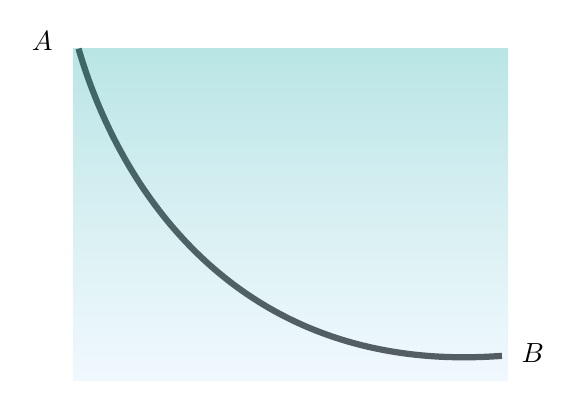
\begin{tikzpicture}[x=0.75pt,y=0.75pt,yscale=-1,xscale=1]
%uncomment if require: \path (0,300); %set diagram left start at 0, and has height of 300

%Curve Lines [id:da20777690252029246] 
\draw [line width=2.25]    (123,70) .. controls (143.99,142.01) and (203.32,227.34) .. (327,218) ;
%Shape: Rectangle [id:dp29650606190117645] 
\draw  [draw opacity=0][shading=_iflcsb4zm,_3o1kvs6si,path fading= _lcv8mc5cx ,fading transform={xshift=2}] (120,70) -- (330,70) -- (330,230) -- (120,230) -- cycle ;

% Text Node
\draw (99,60.4) node [anchor=north west][inner sep=0.75pt]    {$A$};
% Text Node
\draw (335,210.4) node [anchor=north west][inner sep=0.75pt]    {$B$};


\end{tikzpicture}

    \caption{Brachistochrone Represented as Optical Medium}
    \label{fig:Brachistochrone Optical}
\end{figure}

So, with Bernoulli's idea in mind, let us formalute a mathematical description. We will start by showing a modern depiction of Bernoulli's drawing, which I will discuss as we work through the problem. This is shown in \autoref{fig:Brachistochrone Bernoulli}.  The \gls{brachistochrone} curve is denoted with the curve $ABK$. The velocity of the particle as function of height is denoted by the blue curve $AH$, with the magnitude at that height denoted by the horizontal distance from the line $\overline{AC}$. $A$ and $B$, like before, denote the start and end points of the \gls{brachistochrone}.


\begin{figure}[ht]
    \centering

\tikzset{every picture/.style={line width=0.75pt}} %set default line width to 0.75pt        

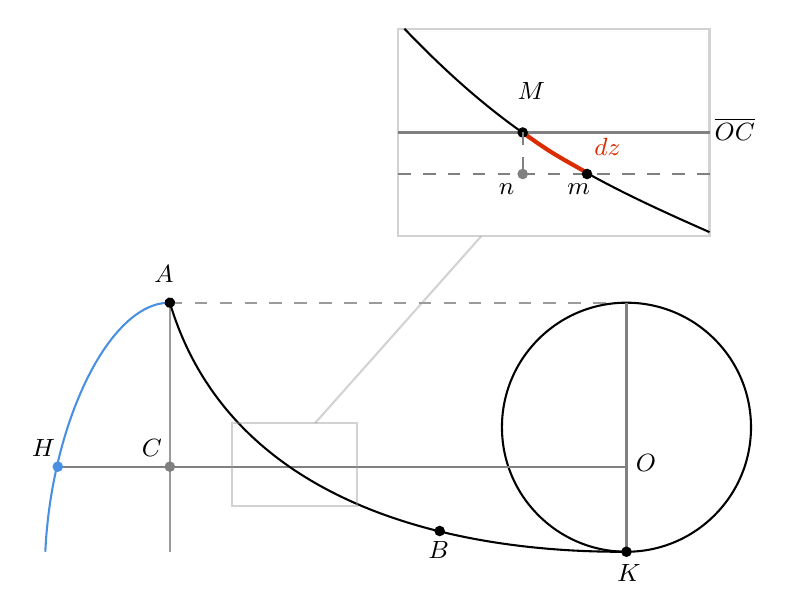
\begin{tikzpicture}[x=0.75pt,y=0.75pt,yscale=-1,xscale=1]
%uncomment if require: \path (0,300); %set diagram left start at 0, and has height of 300

%Straight Lines [id:da10833852271097855] 
\draw [color={rgb, 255:red, 155; green, 155; blue, 155 }  ,draw opacity=1 ] [dash pattern={on 4.5pt off 4.5pt}]  (209,152) -- (429,152) ;
%Curve Lines [id:da5021295458279481] 
\draw [color={rgb, 255:red, 74; green, 144; blue, 226 }  ,draw opacity=1 ]   (209,152) .. controls (179.84,151.72) and (151.84,210.12) .. (149,272) ;
%Shape: Circle [id:dp04643442100307038] 
\draw   (369,212) .. controls (369,178.86) and (395.86,152) .. (429,152) .. controls (462.14,152) and (489,178.86) .. (489,212) .. controls (489,245.14) and (462.14,272) .. (429,272) .. controls (395.86,272) and (369,245.14) .. (369,212) -- cycle ;
%Straight Lines [id:da4186467531833358] 
\draw    (339,262) ;
\draw [shift={(339,262)}, rotate = 0] [color={rgb, 255:red, 0; green, 0; blue, 0 }  ][fill={rgb, 255:red, 0; green, 0; blue, 0 }  ][line width=0.75]      (0, 0) circle [x radius= 2.01, y radius= 2.01]   ;
%Straight Lines [id:da8938403817574153] 
\draw [color={rgb, 255:red, 128; green, 128; blue, 128 }  ,draw opacity=1 ]   (429,152) -- (429,272) ;
%Straight Lines [id:da8730461996297206] 
\draw [color={rgb, 255:red, 128; green, 128; blue, 128 }  ,draw opacity=1 ]   (155,231) -- (429,231) ;
%Straight Lines [id:da39714506859684306] 
\draw [color={rgb, 255:red, 155; green, 155; blue, 155 }  ,draw opacity=1 ]   (209,152) -- (209,272) ;
%Curve Lines [id:da24877719413783894] 
\draw    (209,152) .. controls (238.24,250.12) and (347.04,272.52) .. (429,272) ;
\draw [shift={(209,152)}, rotate = 73.41] [color={rgb, 255:red, 0; green, 0; blue, 0 }  ][fill={rgb, 255:red, 0; green, 0; blue, 0 }  ][line width=0.75]      (0, 0) circle [x radius= 2.01, y radius= 2.01]   ;
%Straight Lines [id:da6942131018955847] 
\draw [color={rgb, 255:red, 155; green, 155; blue, 155 }  ,draw opacity=0.45 ]   (359,120) -- (279,210) ;
%Shape: Rectangle [id:dp7342305689582604] 
\draw  [color={rgb, 255:red, 155; green, 155; blue, 155 }  ,draw opacity=0.45 ] (239,210) -- (299,210) -- (299,250) -- (239,250) -- cycle ;
%Shape: Rectangle [id:dp7388601050866793] 
\draw  [color={rgb, 255:red, 155; green, 155; blue, 155 }  ,draw opacity=0.45 ] (319,20) -- (469,20) -- (469,120) -- (319,120) -- cycle ;
%Straight Lines [id:da9882885067136051] 
\draw [color={rgb, 255:red, 128; green, 128; blue, 128 }  ,draw opacity=1 ]   (319,70) -- (469,70) ;
%Curve Lines [id:da7784742509656426] 
\draw    (322,20) .. controls (372.64,72.92) and (410.24,92.12) .. (469,118) ;
%Straight Lines [id:da9415670416334097] 
\draw [color={rgb, 255:red, 128; green, 128; blue, 128 }  ,draw opacity=1 ][line width=0.75]  [dash pattern={on 4.5pt off 4.5pt}]  (319,90) -- (469,90) ;
%Curve Lines [id:da28920502828750827] 
\draw [color={rgb, 255:red, 218; green, 44; blue, 0 }  ,draw opacity=1 ][line width=1.5]    (379,70) .. controls (393.71,80.73) and (397.71,82.33) .. (411,90) ;
%Straight Lines [id:da04174893208828001] 
\draw    (379,70) ;
\draw [shift={(379,70)}, rotate = 0] [color={rgb, 255:red, 0; green, 0; blue, 0 }  ][fill={rgb, 255:red, 0; green, 0; blue, 0 }  ][line width=0.75]      (0, 0) circle [x radius= 2.01, y radius= 2.01]   ;
%Straight Lines [id:da18742414177909505] 
\draw    (410,90) ;
\draw [shift={(410,90)}, rotate = 0] [color={rgb, 255:red, 0; green, 0; blue, 0 }  ][fill={rgb, 255:red, 0; green, 0; blue, 0 }  ][line width=0.75]      (0, 0) circle [x radius= 2.01, y radius= 2.01]   ;
%Straight Lines [id:da1580581124462085] 
\draw [color={rgb, 255:red, 128; green, 128; blue, 128 }  ,draw opacity=1 ] [dash pattern={on 4.5pt off 4.5pt}]  (379,70) -- (379,90) ;
%Straight Lines [id:da4349956438306438] 
\draw [color={rgb, 255:red, 128; green, 128; blue, 128 }  ,draw opacity=1 ]   (379,90) ;
\draw [shift={(379,90)}, rotate = 0] [color={rgb, 255:red, 128; green, 128; blue, 128 }  ,draw opacity=1 ][fill={rgb, 255:red, 128; green, 128; blue, 128 }  ,fill opacity=1 ][line width=0.75]      (0, 0) circle [x radius= 2.01, y radius= 2.01]   ;
%Straight Lines [id:da8642935211536492] 
\draw    (429,272) ;
\draw [shift={(429,272)}, rotate = 0] [color={rgb, 255:red, 0; green, 0; blue, 0 }  ][fill={rgb, 255:red, 0; green, 0; blue, 0 }  ][line width=0.75]      (0, 0) circle [x radius= 2.01, y radius= 2.01]   ;
%Straight Lines [id:da5335808398156509] 
\draw [color={rgb, 255:red, 128; green, 128; blue, 128 }  ,draw opacity=1 ]   (209,231) ;
\draw [shift={(209,231)}, rotate = 0] [color={rgb, 255:red, 128; green, 128; blue, 128 }  ,draw opacity=1 ][fill={rgb, 255:red, 128; green, 128; blue, 128 }  ,fill opacity=1 ][line width=0.75]      (0, 0) circle [x radius= 2.01, y radius= 2.01]   ;
%Straight Lines [id:da9917624511792703] 
\draw [color={rgb, 255:red, 74; green, 144; blue, 226 }  ,draw opacity=1 ]   (155,231) ;
\draw [shift={(155,231)}, rotate = 0] [color={rgb, 255:red, 74; green, 144; blue, 226 }  ,draw opacity=1 ][fill={rgb, 255:red, 74; green, 144; blue, 226 }  ,fill opacity=1 ][line width=0.75]      (0, 0) circle [x radius= 2.01, y radius= 2.01]   ;

% Text Node
\draw (200,132.4) node [anchor=north west][inner sep=0.75pt]  [font=\small]  {$A$};
% Text Node
\draw (332,265.4) node [anchor=north west][inner sep=0.75pt]  [font=\small]  {$B$};
% Text Node
\draw (375,44.4) node [anchor=north west][inner sep=0.75pt]  [font=\small]  {$M$};
% Text Node
\draw (399,93) node [anchor=north west][inner sep=0.75pt]  [font=\small]  {$m$};
% Text Node
\draw (412,71.4) node [anchor=north west][inner sep=0.75pt]  [font=\small,color={rgb, 255:red, 218; green, 44; blue, 0 }  ,opacity=1 ]  {$dz$};
% Text Node
\draw (423,276.4) node [anchor=north west][inner sep=0.75pt]  [font=\small]  {$K$};
% Text Node
\draw (432,223.4) node [anchor=north west][inner sep=0.75pt]  [font=\small]  {$O$};
% Text Node
\draw (194,216.4) node [anchor=north west][inner sep=0.75pt]  [font=\small]  {$C$};
% Text Node
\draw (366,93) node [anchor=north west][inner sep=0.75pt]  [font=\small]  {$n$};
% Text Node
\draw (141,216.4) node [anchor=north west][inner sep=0.75pt]  [font=\small]  {$H$};
% Text Node
\draw (470,61.4) node [anchor=north west][inner sep=0.75pt]  [font=\small]  {$\overline{OC}$};

\end{tikzpicture}

    \caption{Depiction of John Bernoulli's Brachistochrone Set-Up}
    \label{fig:Brachistochrone Bernoulli}
\end{figure}



Next, we find the differential element, $dz$. This is given by the vertical component ($\hat{x}$-direction in our established coordinates), which is given by the length $\overline{Mn}$, and the horizontal component ($\hat{y}$-direction), $\overline{nm}$. Denoting these distances $dx$ and $dy$, we have the fundemental relation:
\begin{equation}\label{eq:pathlength}
    dz^2=dx^2+dy^2
\end{equation}
Next, he uses the relationship from Snell's Law:
$$n\sin\theta=const.$$
The quantity $\sin\theta$ is thus $\frac{dy}{dz}$ and $n$ some arbitrary value depending on the exact curve.

Remembering that the optical density is inversely proportional to the velocity at a point, Bernoulli relates the horizontal and path length distance to the velocity as well, using the previously established relationship that $\sin\theta=\frac{dy}{dz}$:
$$\frac{dy}{dz}=\frac{v}{n}$$
Using the fact relation from \eqautoref{eq:pathlength}, this can be related to $\frac{dy}{dx}$:
$$\frac{dy}{dx}=\frac{v}{\sqrt{n^2-v^2}}$$
There is one final step in this derivation. Using the fact from before that the velocity of the particle is $v=\sqrt{nx}$, the problem can be solved for a particle acted upon by gravity. Rearrangement yields:
\begin{equation}
\frac{dy}{dx}=\frac{\sqrt{nx}}{\sqrt{n^2-nx}}
\end{equation}
Which can be further simplified by dividing out a $\sqrt{n}$ term:
\begin{equation}
        \frac{dy}{dx}=\sqrt{\frac{x}{n-x}}
\end{equation}
From here, it is simply a matter of solving the differential equation to yield the resulting curve. Performing separation of variables and integrating, we arrive at the final solution:
$$a\tan^{-1}\left(\sqrt{\frac{x}{n-x}}\right)-(n-x)\sqrt{\frac{x}{n-x}}$$
This curve is the curve of a cycloid, the curve generated by tracking a point on a circle which rolls without slipping.

The cycloid, Bernoulli noted, also has some other interesting properties which are strongly connected with the \gls{brachistochrone}. Huygens, another famous mathematician and physicist, had found earlier that a pendulum with a cycloidal path is \textit{isochronous}, meaning that the time for a swing of the pendulum is indepenent of the amplitude. Similarly, for the \gls{brachistochrone}, a particle released at any point along the curve will reach point $B$ at exactly the same time.

%include some graphs of curve and some cool facts about it - same time from any point, pendulum with cycloidal path, Huygens, etc.

It is at this point that we have sufficient background to understand the work that led to the creation of the calculus of variations. From these foundations, mathematicians such as Euler and Lagrange built up a rigorous basis for the subject, which we will now explore in the next chapter.

\newpage

\printendnotes

\chapter{Calculus of Variations}\label{chap:calculus of variations}

\color{red} This chapter needs to be expanded quite a bit, it is definitely lacking in the current state. Maybe include Lagrangian multipliers and problems of the 1st and 2nd variation. Finish the brachistochrone derivation. 
\color{black}

\begin{chapquote}{Richard Feynman}
 ''Nature uses only the longest threads to weave her patterns, so that each small piece of her fabric reveals the organization of the entire tapestry.''
\end{chapquote}

The calculus of variations underpins the ideas of \gls{Lagrangian} and \gls{Hamiltonian} mechanics, so it is important to understand the principles behind it before moving on to the actual mechanics. In analogy to how single variable calculus is fundamental to Newtonian mechanics, the calculus of variations is fundamental to energy mechanics.

The fundamental idea of the calculus of variations is simple. We want to find the maximums and minimums of some quantity in our problem. Why? In physics, we often see that quantities are minimized or maximized for some reason. For example, a soap surface will minimize its surface area, or a beam of photons will follow a \gls{geodesic} of spacetime. Light will also refract through surfaces to minimize time as we have seen in Fermat's least time principle. As we will see, all of mechanics can be understood by the fact that a quantity called the \textit{action} can also be minimized.

Because so many physical phenomena are governed by this behavior to minimize certain quantities, the calculus of variations became a prominent field of study from the 17th through the 20th centuries. Of course, the calculus of variations also has many applications outside of these confines, some of which will be explored at the end of this chapter. The key component of this theory that we need for energy mechanics is called the Euler-Lagrange equation, which we will now derive.

\section{Derivation of the Euler-Lagrange Equation}

As stated before, for an optimization problem, we need to find the minima or maxima of a quantity. In single variable calculus, we only concern ourselves with finding the minimum value of a function, say finding the minimum value of $x^2$. Here however, we now have a new challenge. That challenge to find a whole function which is a minimum.

Stated more precisely, we are attempting to find a function that is the minimum for some set of conditions. The conditions are often posed as conditions on a function or its derivative. We may write the conditions generally as $y(x)$ and $y'(x)$.

These conditions take the form of a function, as they are dependent on some variable $x$. The tricky part about variational calculus is that we need to find another function, $f$, which abides by these constraint equations, but is also a minimum! Since $f$ has a dependence on these constraints, we may generally write $f$ as:
$$f[y(x),y'(x);x]$$
This statement means that $f$ is a function which is defined by $y(x)$ and its derivative $y'(x)$. The semicolon notes that the variable of interest is $x$.

We may write a function $f$ which abides by these conditions, say $f = y(x)+2y'(x)$. That is fine, but how can we find where this function is minimum? What does that even mean?

Since our function exists over a whole range of values of $x$, the sensible thing to do is to consider the function $f$ over all values of $x$, and assign a value to it that way. Of course, we can do this quite easily with an integral! We can evaluate this at two set endpoints, $x_1$ and $x_2$, and this will return a single number value that represents the function! We call this scalar output a \gls{functional}. This \gls{functional} is essentially a function of $f$, so it is a function of a function!

We typically describe a functional with the letter $J$, and we write the form of the integral as:
\begin{equation}\label{eq:functional}
    J=\int_{x_1}^{x_2}f\left[y(x),y'(x);x\right]{dx}
\end{equation}
Remember that the most important aspect of $J$ is that we have taken an entire function, over a fixed range, and collapsed all of that functions properties into a single number, $J$! We may say this more precisely as: The \gls{functional}, $J$, is a quantity which maps a function onto the real number line. This means that it takes the function as its input and outputs a single real number (that is, a function of a function). 

This, in essence, is the calculus of variations. For our purposes, we only want a specific application, which is to solve optimization problems to find the minima of functions. That is, we are attempting to find conditions on the function, $y(x)$ and $y'(x)$, which yield an extrema of $J$. 

\newglossaryentry{neigh func}
{
    name=neighborhood function,
    first = {\textit{neighborhood function}},
    description={A small function added to another function in the calculus of variations. Analogous to a differential element in single variate calculus}
}

\subsubsection{Extrema conditions}
To find the extrema of the function is quite similar to the approach we would take in single variate calculus. We are all familiar with the method by which is this accomplished in single variable calculus. To find the minima or maxima of a function $f(x)$, we find where $f'(x)=0$ (\autoref{fig:single var func}).
\begin{figure}[ht]
    \centering


\tikzset{every picture/.style={line width=0.75pt}} %set default line width to 0.75pt        

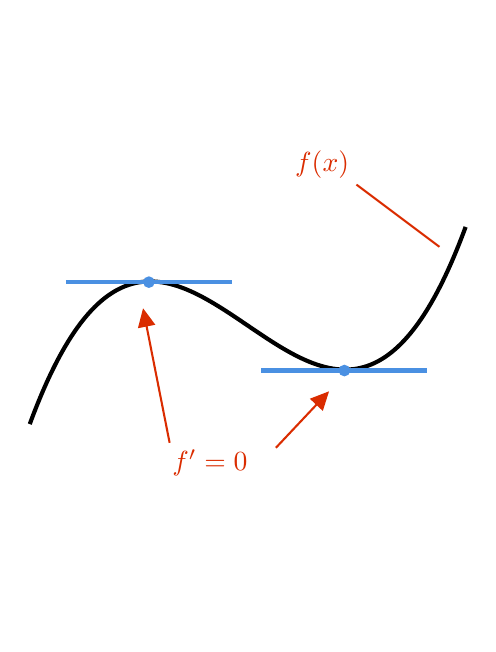
\begin{tikzpicture}[x=0.75pt,y=0.75pt,yscale=-1,xscale=1]
%uncomment if require: \path (0,300); %set diagram left start at 0, and has height of 300

%Shape: Polynomial [id:dp31740373171286806] 
\draw  [line width=1.5]  (137,222) .. controls (207,32) and (277,317) .. (347,127) ;
%Straight Lines [id:da15243145724705576] 
\draw [color={rgb, 255:red, 74; green, 144; blue, 226 }  ,draw opacity=1 ][line width=1.5]    (248.6,196.2) -- (328.6,196.2) ;
\draw [shift={(288.6,196.2)}, rotate = 0] [color={rgb, 255:red, 74; green, 144; blue, 226 }  ,draw opacity=1 ][fill={rgb, 255:red, 74; green, 144; blue, 226 }  ,fill opacity=1 ][line width=1.5]      (0, 0) circle [x radius= 1.74, y radius= 1.74]   ;
%Straight Lines [id:da29067177346887385] 
\draw [color={rgb, 255:red, 218; green, 44; blue, 0 }  ,draw opacity=1 ]   (255.59,233.41) -- (279.13,208.4) ;
\draw [shift={(281.19,206.21)}, rotate = 133.26] [fill={rgb, 255:red, 218; green, 44; blue, 0 }  ,fill opacity=1 ][line width=0.08]  [draw opacity=0] (8.93,-4.29) -- (0,0) -- (8.93,4.29) -- cycle    ;
%Straight Lines [id:da5077584687934987] 
\draw [color={rgb, 255:red, 218; green, 44; blue, 0 }  ,draw opacity=1 ]   (334.4,136.6) -- (294.4,106.6) ;
%Straight Lines [id:da6280064979254578] 
\draw [color={rgb, 255:red, 74; green, 144; blue, 226 }  ,draw opacity=1 ][line width=1.5]    (154.4,153.6) -- (234.4,153.6) ;
\draw [shift={(194.4,153.6)}, rotate = 0] [color={rgb, 255:red, 74; green, 144; blue, 226 }  ,draw opacity=1 ][fill={rgb, 255:red, 74; green, 144; blue, 226 }  ,fill opacity=1 ][line width=1.5]      (0, 0) circle [x radius= 1.74, y radius= 1.74]   ;
%Straight Lines [id:da1070293344802159] 
\draw [color={rgb, 255:red, 218; green, 44; blue, 0 }  ,draw opacity=1 ]   (204.39,231.01) -- (192.17,169.16) ;
\draw [shift={(191.59,166.21)}, rotate = 78.83] [fill={rgb, 255:red, 218; green, 44; blue, 0 }  ,fill opacity=1 ][line width=0.08]  [draw opacity=0] (8.93,-4.29) -- (0,0) -- (8.93,4.29) -- cycle    ;

% Text Node
\draw (204.2,232.8) node [anchor=north west][inner sep=0.75pt]  [color={rgb, 255:red, 218; green, 44; blue, 0 }  ,opacity=1 ]  {$f'=0$};
% Text Node
\draw (263.4,89) node [anchor=north west][inner sep=0.75pt]  [color={rgb, 255:red, 218; green, 44; blue, 0 }  ,opacity=1 ]  {$f( x)$};


\end{tikzpicture}

    \caption{Extrema of a single variable function}
    \label{fig:single var func}
\end{figure}
What is important to note is what happens right around these extremal points. If we are right at the point where $f'(0)$, we are of course at a local minimum or maximum of the function. However, if we move left or right by some very small amount -- which we call $\varepsilon$ -- the value of the function stays the same! This should come as no suprise, because $f'(x)$ gives a local value of the tangent of the function. In other words, it gives a linear approximation of the function at that location. As long as $\varepsilon$ remains small, $f(x)$ is perfectly represented by this linear approximation.

Now, we may extend this definition to the more difficult case of the extrema in variational calculus. Instead of adding some small value, we are instead adding some small function. This function is typically denoted $\eta(x)$, and by convention we still multiply $\eta(x)$ by $\varepsilon$ to denote the fact that we are considering very small functions.

In analogy to the single variable case of a minimum, if we have a minimized functional, we can add $\varepsilon\eta(x)$ to $y(x)$ and the value of the functional remains unchanged! We can see this in \autoref{fig:neigh func}.

\begin{figure}[ht]
    \centering


\tikzset{every picture/.style={line width=0.75pt}} %set default line width to 0.75pt        

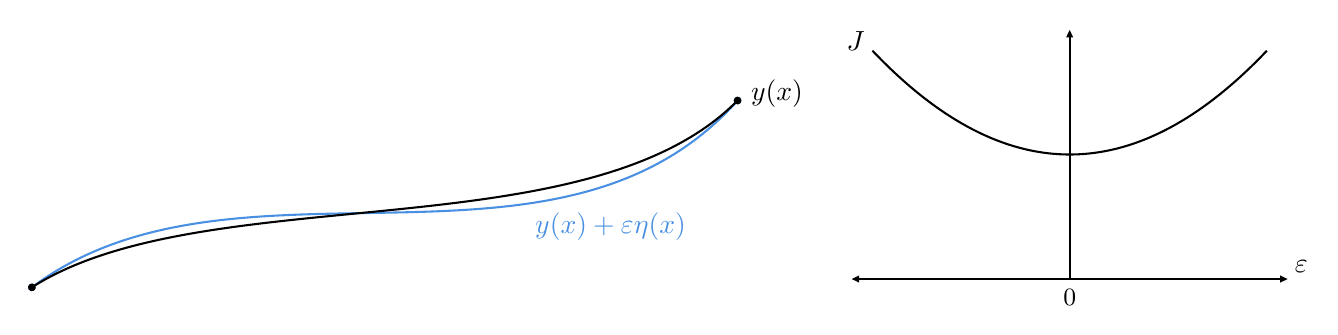
\begin{tikzpicture}[x=0.75pt,y=0.75pt,yscale=-1,xscale=1]
%uncomment if require: \path (0,300); %set diagram left start at 0, and has height of 300

%Curve Lines [id:da3860827164688039] 
\draw [color={rgb, 255:red, 74; green, 144; blue, 226 }  ,draw opacity=1 ]   (25,214) .. controls (122.59,140.96) and (278.59,220.96) .. (365,124) ;
\draw [shift={(365,124)}, rotate = 311.71] [color={rgb, 255:red, 74; green, 144; blue, 226 }  ,draw opacity=1 ][fill={rgb, 255:red, 74; green, 144; blue, 226 }  ,fill opacity=1 ][line width=0.75]      (0, 0) circle [x radius= 1.34, y radius= 1.34]   ;
\draw [shift={(25,214)}, rotate = 323.19] [color={rgb, 255:red, 74; green, 144; blue, 226 }  ,draw opacity=1 ][fill={rgb, 255:red, 74; green, 144; blue, 226 }  ,fill opacity=1 ][line width=0.75]      (0, 0) circle [x radius= 1.34, y radius= 1.34]   ;
%Curve Lines [id:da7977961164869156] 
\draw    (25,214) .. controls (108.39,160.8) and (292.39,197.6) .. (365,124) ;
\draw [shift={(365,124)}, rotate = 314.61] [color={rgb, 255:red, 0; green, 0; blue, 0 }  ][fill={rgb, 255:red, 0; green, 0; blue, 0 }  ][line width=0.75]      (0, 0) circle [x radius= 1.34, y radius= 1.34]   ;
\draw [shift={(25,214)}, rotate = 327.46] [color={rgb, 255:red, 0; green, 0; blue, 0 }  ][fill={rgb, 255:red, 0; green, 0; blue, 0 }  ][line width=0.75]      (0, 0) circle [x radius= 1.34, y radius= 1.34]   ;
%Straight Lines [id:da527720029795286] 
\draw    (423,210) -- (627,210) ;
\draw [shift={(630,210)}, rotate = 180] [fill={rgb, 255:red, 0; green, 0; blue, 0 }  ][line width=0.08]  [draw opacity=0] (3.57,-1.72) -- (0,0) -- (3.57,1.72) -- cycle    ;
\draw [shift={(420,210)}, rotate = 0] [fill={rgb, 255:red, 0; green, 0; blue, 0 }  ][line width=0.08]  [draw opacity=0] (3.57,-1.72) -- (0,0) -- (3.57,1.72) -- cycle    ;
%Straight Lines [id:da4291618420656924] 
\draw    (525,93) -- (525,210) ;
\draw [shift={(525,90)}, rotate = 90] [fill={rgb, 255:red, 0; green, 0; blue, 0 }  ][line width=0.08]  [draw opacity=0] (3.57,-1.72) -- (0,0) -- (3.57,1.72) -- cycle    ;
%Shape: Parabola [id:dp32441741010727465] 
\draw   (430,100) .. controls (493.33,166.67) and (556.67,166.67) .. (620,100) ;

% Text Node
\draw (370,112.4) node [anchor=north west][inner sep=0.75pt]    {$y( x)$};
% Text Node
\draw (266,176.4) node [anchor=north west][inner sep=0.75pt]  [color={rgb, 255:red, 74; green, 144; blue, 226 }  ,opacity=1 ]  {$y( x) +\varepsilon \eta ( x)$};
% Text Node
\draw (416,89.4) node [anchor=north west][inner sep=0.75pt]    {$J$};
% Text Node
\draw (632,199.4) node [anchor=north west][inner sep=0.75pt]    {$\varepsilon $};
% Text Node
\draw (525,213.4) node [anchor=north] [inner sep=0.75pt]  [font=\small]  {$0$};

\end{tikzpicture}
    \caption{Graphical representation of the neighborhood function}
    \label{fig:neigh func}
\end{figure}

We can see this playing the same role as it did in the single variable case. As $\varepsilon$ tends to zero, the functional approaches the minimum value (shown in the RHS of \autoref{fig:neigh func})! The calculus of variations has some special terminology to define these properties which we should discuss now. These special values where $J$ is minimized are called \textit{stationary points}. We call them this because of the fact we can add some $\varepsilon\eta(x)$ and they are unchanged! For values that are not the minimum of $J$, this condition does not hold.

Typically we also call $\eta(x)$ the \gls{neigh func}. The function $\eta(x)$ must meet the condition that is has zero value at the endpoints of the integral, $x_1$ and $x_2$. Otherwise, there is no guarantee that $\varepsilon\eta(x)$ will converge to the correct answer! It will also prove useful later when we go to integrate our function.

The \gls{neigh func} proves especially useful because we can use the criteria of a stationary point of $J$ to find solutions of $y(x)$ satisfying this!

We often compactly write $y(x)+\varepsilon\eta(x)$ as $y(\varepsilon,x)$. We define the condition $y(0,x)\equiv y(x)$, where $y(x)$ is the function that gives the extrema of $J$. So, we can write $y(\varepsilon,x)$ as:
\begin{equation}\label{eq:y epsilon}
    y(\varepsilon,x)=y(0,x)+\varepsilon\eta(x)
\end{equation}
The other important condition is that both $y(x)$ and $\eta(x)$ must have a continuous first derivative so that $y'(\varepsilon,x)$ can be defined:
\begin{equation}\label{eq:y prime epsilon}
    y'(\varepsilon,x)=\frac{dy(0,x)}{dx}+\varepsilon\frac{d\eta}{dx}
\end{equation}
Now, we have all of the components that we need to evaluate our original equation for $J$ in terms of $y(\varepsilon,x)$.

\subsubsection{Solving for stationary points}

Using this definition of the \gls{neigh func}, we can apply it to \eqautoref{eq:functional} to write the more general form as:
\begin{equation}\label{eq:neighborhood functional}
    J(\varepsilon)=\int_{x_1}^{x_2}f\left[y(\varepsilon,x),y'(\varepsilon,x);x\right]{dx}
\end{equation}
So, with this new version of the function, we can finally find the extrema using the familiar calculus rule, setting the derivative of $J$ equal to zero. We also evaluate this condition $\varepsilon=0$ since we defined the extrema to exist at $y(0)$:
\begin{equation}
    \left.\frac{\partial J(\varepsilon)}{\partial\varepsilon}\right\vert_{\varepsilon=0}=0
\end{equation}
Applying this to \eqautoref{eq:functional}, we arrive at
\begin{equation}\label{eq:neighborhood functional diff}
    \frac{\partial J(\varepsilon)}{\partial\varepsilon}= \frac{\partial}{\partial\varepsilon}\int_{x_1}^{x_2}f\left[y(0,x),y'(0,x);x\right]{dx}
\end{equation}
The $\varepsilon$ terms drop out from the RHS from the evaluation of $\varepsilon=0$. Applying the Leibniz integral rule, the partial derivative can be moved inside the RHS integral:
\begin{equation}
    \frac{\partial J(\varepsilon)}{\partial\varepsilon}= \int_{x_1}^{x_2}\frac{\partial}{\partial\varepsilon}f\left[y(x),y'(x);x\right]{dx}
\end{equation}
Applying the rules of implicit integration on the integrand, we get:
\begin{equation}\label{eq:diff functional}
    \frac{\partial J(\varepsilon)}{\partial\varepsilon}= \int_{x_1}^{x_2}f\left(\frac{\partial f}{\partial y}\frac{\partial y}{\partial\varepsilon}+\frac{\partial f}{\partial y'}\frac{\partial y'}{\partial\varepsilon}\right){dx}
\end{equation}
Note that we still must take the partial derivative with respect to $\varepsilon$ on the RHS, even though we have plugged in 0 for $\varepsilon$. This is because these are still functions of $\varepsilon$, even after plugging in values of 0.

Next, we can find expressions for $\frac{\partial y}{\partial \varepsilon}$ and $\frac{\partial y'}{\partial \varepsilon}$. This is done with the expressions \eqautoref{eq:y epsilon} and \eqautoref{eq:y prime epsilon}. Starting with the first, we differentiate \eqautoref{eq:y epsilon} with respect to $\varepsilon$:
\begin{equation}\label{eq:y diff epsilon}
    \frac{\partial}{\partial \varepsilon}y(\varepsilon,x)=\frac{\partial}{\partial \varepsilon}\left[y(0,x)+\varepsilon\eta(x)\right]
\end{equation}
Here, $y(0,x)$ is independent of $\varepsilon$ since we define it to occur at value $\varepsilon=0$. So this leaves us with
\begin{equation}\label{eq:diff y diff epsilon}
     \frac{\partial y}{\partial \varepsilon}= \eta(x)
\end{equation}
Doing the same for \eqautoref{eq:y prime epsilon}, we arrive at
\begin{equation}\label{diff y' diff epsilon}
     \frac{\partial y'}{\partial \varepsilon}= \frac{\partial \eta}{\partial x}
\end{equation}
Finally, plugging these back into the original expression for \eqautoref{eq:diff functional}, we get the expression
\begin{equation}\label{eq:diff functional subs}
    \frac{\partial J(\varepsilon)}{\partial\varepsilon}= \int_{x_1}^{x_2}\left(\frac{\partial f}{\partial y}\eta(x)+\frac{\partial f}{\partial y'}\frac{\partial \eta}{\partial x}\right){dx}
\end{equation}
Finally, performing integration by parts on the RHS to simplify, we arrive at the final integral expression:
\begin{equation}\label{eq:diff functional final}
    \frac{\partial J(\varepsilon)}{\partial\varepsilon}= \int_{x_1}^{x_2}\left(\frac{\partial f}{\partial y}-\frac{d}{dx}\frac{\partial f}{\partial y'}\right)\eta(x){dx}
\end{equation}
Since we are evaluating the extrema, $\frac{\partial J(\varepsilon)}{\partial\varepsilon}$ evaluates to 0. This leaves us with the final form of the expression, which will give us the useful result we have been looking for:
\begin{equation}
    0= \int_{x_1}^{x_2}\left(\frac{\partial f}{\partial y}-\frac{d}{dx}\frac{\partial f}{\partial y'}\right)\eta(x){dx}
\end{equation}

Since $\eta(x)$ is an arbitrary function, the only way to guarantee equality is to ensure that the integrand part in parentheses is 0.

\newglossaryentry{Euler Equation}
{
    name=Euler's equation,
    first = {\textit{Euler's equation}},
    description={The fundemental equation in the calculus of variations describing the maximum or minimum conditions of a functional},
    see={functional}
}

This gives us the fundamental equation of the calculus of variations, called \gls{Euler Equation}:
\begin{gather}\label{eq: Euler's Diff eq}
\color{blue}\boxed{\color{black}\frac{\partial f}{\partial y}-\frac{d}{dx}\frac{\partial f}{\partial y'}=0}\\
\color{blue}\mathrm{Euler's \ Equation}
\end{gather}
\subsection{Delta Notation}
In later sections, it is useful to have a shorthand for these partial derivative quantities. For a quantity $\chi$, the variation, $\delta$ is given as:
$$\delta\chi\equiv\frac{\partial\chi}{\partial \varepsilon}d\varepsilon$$Using this notation, we can rewrite \eqautoref{eq:diff functional final} after some algebraic manipulation as:
\begin{equation}
    \delta J= \int_{x_1}^{x_2}\left(\frac{\partial f}{\partial y}-\frac{d}{dx}\frac{\partial f}{\partial y'}\right)\delta y{dx}
\end{equation}
And thus, \eqautoref{eq: Euler's Diff eq} can be written concisely as:
\begin{equation}
    {\color{black}\delta J=0}
\end{equation}
This is a very general and far reaching conclusion that can be applied to many systems. For our use cases in dynamics, we have more useful forms of this equation which will be explored in the following sections.

\section{Using Variational Calculus}
A vast majority of the use cases of variational calculus are solving optimization problems. For this purpose, we will use the \gls{Euler Equation} extensively. 

\subsection{Geodesics}
We will explore a short example of its usefulness here as it relates to problems in geometry - namely of the \glspl{geodesic} of spherical geometries.

\begin{example}[Geodesics of a Sphere]\label{ex:geodesic}
To show an example of the use of variational calculus, we will consider finding the shortest path of a spherical surface. We know from intuition that this path is a great circle. Let us prove this mathematically with variational calculus:

To start, we need to define what an arc length on a spherical surface looks like. In general, we have the formula for arc length that $ds^2=dx^2+dy^2+dz^2$. We can use the standard spherical coordinates:
    $$\begin{array}{l}
        x=r\sin\theta\cos\theta\\
        y=rsin\theta\sin\phi\\
        z=r\cos\phi
    \end{array}$$
Some long and arduous mathematics gives the following for the arc length:
$$ds=\sqrt{r^2d\theta^2+r^2\sin^2\theta d\phi^2}$$
At this point, we want to make two assumptions to get this into a form that we can easily evaluate. Since we are only looking for a \gls{geodesic}, we can assume that $r=1$ without losing any information. Next, we want to put our solution in terms of just one variable - either $d\theta$ or $d\phi$. In this case, I choose $d\theta$. This means that we parameterize our path with $\phi=\phi(\theta)$. Taking this derivative, we have:
$$\phi'=\frac{d\phi}{d\theta}$$
This gives ${\phi'}^2=\frac{d\phi^2}{d\theta^2}$. Rewriting with these new terms, we have an expression for $ds$:
$$ds=\sqrt{1+\sin^2\theta{\phi'}^2}d\theta$$
To get the total arc length, we simply integrate this path over the desired path.
$$S=\int_{\theta_1}^{\theta_2}{\sqrt{1+\sin^2\theta{\phi'}^2}d\theta}$$

Up to here, the problem has been mostly set-up. Now, we apply the variational principles to find the minimum. In this case, $S$ is our functional which should be minimized to give the minimum length, that is, to find $\delta S=0$.

We take our function $f$ to be $\sqrt{1+\sin^2\theta{\phi'}^2}$ and apply the Euler equation:
$$\frac{\partial f}{\partial \phi}=\frac{d}{d\theta}\frac{\partial f}{\partial \phi'}$$

Note that $\phi$ has replaced $y$ in the form presented in \eqautoref{eq: Euler's Diff eq}, $\phi'$ has replaced $y'$, and $\theta$ has replaced $x$. The fundamental nature of the equation is identical.

Now, we simply perform the calculus to find our answer:
$$\frac{\partial f}{\partial \phi}=\frac{\partial}{\partial\phi}\left(\sqrt{1+\sin^2\theta{\phi'}^2}\right)=0$$
We find that this first expression is 0 since there are no terms containing $\phi$ explicitly. This means that the derivative of $\frac{\partial f}{\partial \phi'}$, $\frac{d}{d\theta}\frac{\partial f}{\partial \phi'}$, must be constant with respect to $\theta$ so that its derivative is 0. We will use this fact below. We establish the whole term as:

$$\frac{d}{d\theta}\frac{\partial f}{\partial \phi'}=\frac{d}{d\theta}\left[\frac{\partial}{\partial \phi'}\left(\sqrt{1+\sin^2\theta{\phi'}^2}\right)\right]=0$$
Computing the partial derivative, we have:

\begin{equation}
\frac{\partial}{\partial \phi'}\left(\sqrt{1+\sin^2\theta{\phi'}^2}\right)=\frac{\sin^2\theta\phi'}{\sqrt{1+\sin^2\theta\phi'}}=const.
\end{equation}
We can rearrange the statement to solve for the constant (which I will now call $c$) in terms of $\phi'$, which is simply algebraic manipulation.
\begin{equation}
    \begin{split}
      c &=\frac{\sin^2\theta\phi'}{\sqrt{1+\sin^2\theta\phi'}}\\
\sin^2\theta\phi' &= c\sqrt{1+\sin^2\theta\phi'}\\
\sin^4\theta{\phi'}^2 &= c^2\left(1+\sin^2\theta\phi'\right)\\
c^2 &= {\phi'}^2\sin^2\theta\left(\sin^2{\theta}-c^2\right)\\
{\phi'}&=\frac{c}{\sin\theta\left(\sin^2\theta-c^2\right)}
    \end{split}
\end{equation}
We have been using the implicit assumption that $\phi$ is a function of $\theta$, so we finally integrate this with respect to $\theta$ to attain the final \gls{geodesic} curve in terms of $\phi$ and $\theta$.

$$\phi=\int{\phi'}=\int{\frac{c}{\sin\theta\left(\sin^2\theta-c^2\right)}}$$
After looking at the problem for a long time, it becomes apparent that we should perform u-substitution with $u=\cot\theta$. Evaluation of this integral can easily be done with MATLAB or Mathematica (there is no useful information gleaned from doing this integral). Doing so yields: $$\cot{\theta}=a\cos{(\phi-\phi_0)}$$
Where $\phi_0$ comes from the integration constant. This is our final answer. We can solve for $a$ and $\phi_0$ using numerical methods since the equation is transcendental.

A MATLAB Script which shows such \glspl{geodesic} is included in the Appendix in \autoref{script:Geodesic}. The output of the script is shown in \autoref{fig:Geodesic}.

\begin{figure}[H]
    \centering
    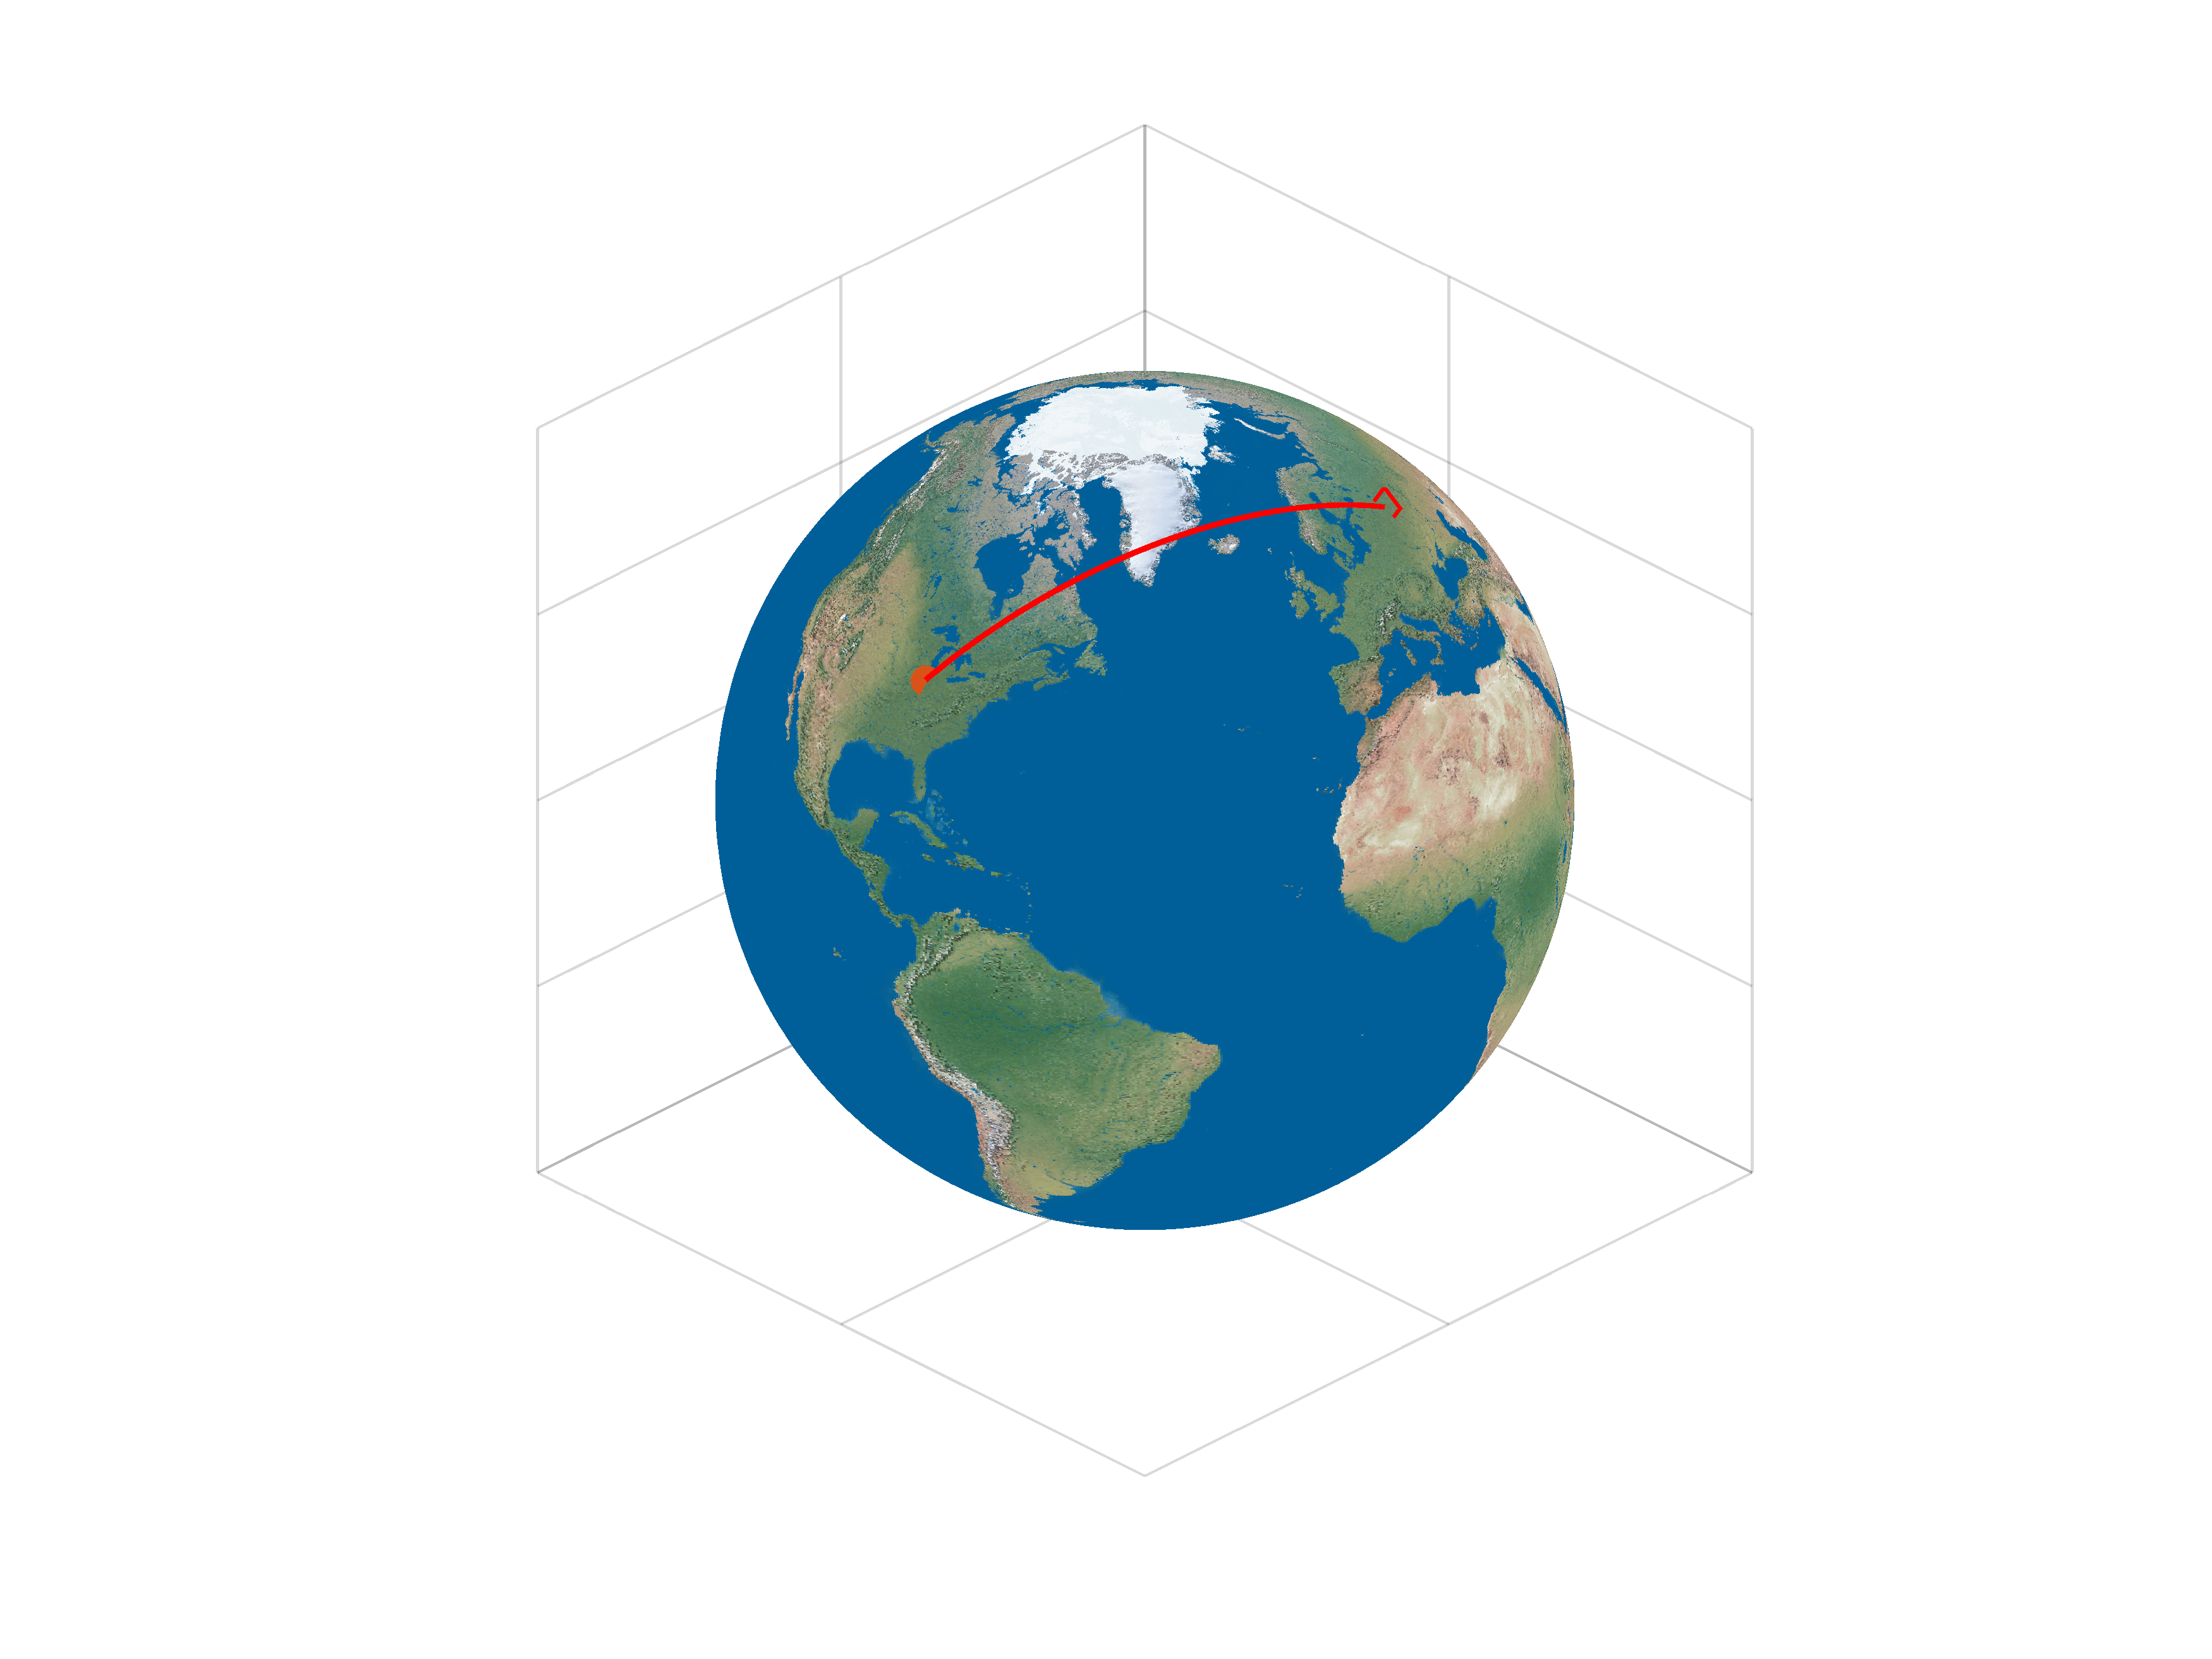
\includegraphics[width=.75\linewidth]{Scripts/Geodesic.png}
    \caption{Geodesic shown on the Earth}
    \label{fig:Geodesic}
\end{figure}

For a short path length where the distance is much smaller than the sphere radius $r$, we expect that this will return the standard straight line as the shortest distance.

Performing a Taylor expansion and keeping only the first-order terms:
$$\frac{1}{\theta}=a$$
So, it is seen that the value $\theta$, as expected, is constant for a short path length. This formula thus returns the standard equation of a line on short scales!

One important consequence of this is that a spherical geometry, when looked at `closely' (this is, looking at an infinitesimal portion of the surface) is locally Euclidean! This fact that the geometry looks locally Euclidean will be important in our later discussions in \autoref{chap:lie theory}.
\end{example}
 
\subsection{Revisiting the Brachistochrone}

\begin{example}[Brachistochrone]\label{ex:brachistrochrone}
    Let us return to the example of the \gls{brachistochrone} to demonstrate the usefulness of the calculus of variations in solving  this problem. Of course, we have seen John

    %clean this up and explain
You are a prominent mathematician in the year 1696. Bernoulli proposes a problem to you to find a curve from a point $(x_0,y_0)$ to another point $\left(x_f,y_f\right)$. When a particle is placed on this path, it should be a faster path than any other path the particle could take down the slope under the influence of only gravity.

Find the velocity as a function of the distance from the initial height, $h$, for the particle using energy conservation.

Write a general expression for the amount of time it takes a particle to descent a path using an integral. \textit{Hint: you can write $t=\frac{ds}{v}$}.

Use the Euler-Lagrange equation to solve for the form of this curve (You may find the integral form useful!). Plot the result.
\end{example}

\chapter{Lagrangian Mechanics}\label{chap:lagrangian}

\color{red} This chapter needs a large amount of work still. Need to finish reading through Goldstein and include neccesary information from there. Include generalized forces, lagrangian multipliers, improve non-holonomic constraints, write the quantuam to lagrangian section, and write some good practice problems.

\color{black}

Energy methods of mechanics use the energy of a system to determine the \gls{eom} of the system . This is in contrast to the Newtonian method, which considers the forces of a system to produce its \gls{eom}. The good news is that both will result in the same answer (see proof in \autoref{equiv newt and lang}). However, having both in your set of tools as an engineer can prove especially useful.

To grasp energy methods, it is best to have an intuition for Newtonian dynamics first. A thorough reading of Volume I and other sources will help prepare the reader for this section. The two are quite different, but the \gls{Lagrangian} formalism deals less with intuition and more with analytical solutions, so having the intuition from the Newtonian approach will be useful.

There are two main types of energy mechanics, referred to as \gls{Hamiltonian} and \gls{Lagrangian} Mechanics. In this chapter, we will mostly focus on the \gls{Lagrangian} version of these mechanics. \gls{Hamiltonian} mechanics will be discussed further in \autoref{chap:hamiltonian}. Both approaches use energy, but have some distinct differences in implementation. Generally, the \gls{Lagrangian} approach is more suited to solving problems in classical dynamics, so we will start with this approach.

\newglossaryentry{symplectic int}
{
    name=symplectic integrator,
    first = {\textit{symplectic integrator}},
    description={A class of numerical integration schemes that are energy preserving because they preserve certain geometric properties of a differential equation}
}

Although the \gls{Hamiltonian} and \gls{Lagrangian} are not directly used in the case of our 6-\gls{dof}, they are fundamental to other areas of mechanics and make derivations far simpler in many cases. The \gls{Hamiltonian} and \gls{Lagrangian} descriptions of mechanics are more often taught to physics students rather than engineers, but we feel that they deserve inclusion among the topics presented here. For the reader interested in applications in robotics, energy mechanics has a vast number of applications.

When we discuss \gls{numerical int}, we can use \glspl{symplectic int} when our problem has a \gls{Hamiltonian} description. This will be further discussed in \autoref{sec: Syplectic Ints}. You may find that certain \gls{eom} derivations, such as the spinning top and problems in orbital mechanics are more easily accomplished with energy methods. Another reason to motivate these systems is that these energy methods are invariant to transformations such as rotations. This occurs because energy methods employ a generalized coordinate system. These generalized coordinates are very powerful and allow us to describe a huge variety of systems. We will see this later in some examples.

A brief overview of the differences between the two schemes of \gls{eom} derivation is shown in \autoref{fig:newt v lang}. As can be seen from the figure, the underlying governing mechanics are no different, but the way in which we arrive at the \gls{eom} is completely different. Knowing this, we can begin our dive into \gls{Lagrangian} mechanics.

\begin{figure}[ht]
    \centering
    
\includesvg[width=.6\linewidth]{Images/NewtonianLagrangian.svg}

    \caption{Newtonian vs. Lagrangian Mechanics Approach}
    \label{fig:newt v lang}
\end{figure}

\section{Hamilton's Principle}
The basis of \gls{Lagrangian} mechanics is Hamilton's Principle. Similar to Fermat's principle of least time, Hamilton's principle states that a quantity called the \gls{action} must be minimized.

Although we may not have a physical intuition of why this is true right now (that will come later), it proves to be especially useful. Additionally, these ideas follow direction from the calculus of variations! Hamilton (alongside some others) formulated a definition of this principle that describes all physical systems. Hamilton's Principle is as follows:
\begin{theorem}[Hamilton's Principle]
In a conservative system which may travel from one point to another within a specific time interval, the path that is followed is the path which minimizes the time integral of the difference between the kinetic and potential energies.
$$\delta \int_{t_1}^{t_2}{T-U}{dt}=0$$
\end{theorem}

The quantity $T-U$, the kinetic energy minus the potential energy, is a quantity called the \gls{Lagrangian}, denoted $L$. 
\begin{equation}
    L\equiv T-U
\end{equation}
The \gls{Lagrangian} typically has no physical meaning. Instead, we simply choose a \gls{Lagrangian} such that the laws of mechanics work. The reason for the negative sign on the potential, $U$, can be seen in the derivation in \autoref{equiv newt and lang}. In short, the negative must be present so that the \gls{Lagrangian} matches the Newtonian description.

Before we get too ahead of ourselves, though, we should investigate this integral a bit further. We can notice that the form of the integral is quite similar to the equations we have seen in the calculus of variations.

In fact, we can notice that the potential energy, generally, is a function of the position, $y$, and the kinetic energy is a function of $y'$ -- the time derivative of the position. As a result, we can write our \gls{Lagrangian} quite generally as:
$$\int_{t_1}^{t_2}f[y(x),y(x)';x]dx$$
This of course, matches the definition for the functional that we described in \autoref{chap:calculus of variations}.

\newglossaryentry{princ of least action}
{
    name=principle of least action,
    first = {\textit{principle of least action}},
    description={A form of Hamilton's Principle that states that the action of a system should be minimized in a physical mechanical system},
    see={action}
}
In the case of \gls{Lagrangian} mechanics, the functional is called the \gls{action}, denoted $S$. This is often why Hamilton's Principle is also called the \gls{princ of least action}.  We can thus equivalently write the integral as:
\begin{equation}
    S=\int_{t_1}^{t_2}{L}{dt}
\end{equation}
So, our \gls{action} takes the form of the \gls{functional} from the calculus of variations. From Hamilton's principle, this \gls{functional}, the \gls{action}, must be minimized. So, we often see the compact form of Hamilton's Principle as:
$$\delta S=0$$
We know from our previous studies that the extremal conditions of a functional can be found using the \gls{Euler Equation}.

\newglossaryentry{euler lagrange}
{
    name=Euler-Lagrange equation,
    first = {\textit{Euler-Lagrange equation}},
    description={The fundemental equation describing the solutions that give the extrema of the action in a Lagrangian system.},
    see={action}
}

Substituting in the variables that we use for the \gls{Lagrangian}, we have the \glspl{euler lagrange}, which is used to find the extremal solutions:
\begin{gather}\label{eq: Euler-Lagrange}
    \color{blue}\boxed{\color{black}\frac{\partial L}{\partial x_i}-\frac{d}{dt}\frac{\partial L}{\partial \dot{x}_i}=0}\\ \mathrm{\color{blue}Euler-Lagrange \ Equations}
\end{gather}
Hamilton's Principle then states that the solutions to this \gls{euler lagrange} are the \gls{eom} of the system!

There is one small part of the principle that I glossed over during the derivation; the fact that the system must be \gls{conservative}. In short, a \gls{conservative} system is one in which the energy of the particle is path-independent. See \cite{goldstein_classical_2008} Chapter 1 for more information. This assumption helped when I assumed that the potential, $U$, was a function of position only. If this potential had a dependence of velocity, then the problem would not be easily solvable.

This does mean that frictional forces and aerodynamics are not modeled with the \gls{Lagrangian} we describe here (although they can be with the utilization of Rayleigh's dissipation function and other techniques, such as those discussed in \cite{rabei_hamiltonian_2004}). This is the reason we do not directly use these equations in the 6-DoF.\footnote{However, much of the rotational dynamics we describe can be represented equivalently using the \gls{Lagrangian} approach, so we do use these equations in a roundabout manner.} This is also one reason that we need to use numerical integration methods to solve the \gls{eom} for the rocket trajectory when using Newtonian dynamics. In fact, the idea that the system in non-\gls{conservative} and cannot be solved analytically are intrinsically linked.

So, for systems that are non-conservative, it is best to stick with the Newtonian method of mechanics, as we do for our 6-DoF, since the methods to find approximate solutions for these equations are quite a bit simpler. 

However, for systems that are frictionless, the methods described here will work well. While it may seem that frictionless systems are very idealistic, we do see systems that can be approximated as frictionless quite often! Orbits, of course, are one case where this is especially true. For many other systems, such as a spinning top or other rotating bodies, we can often ignore the small amount of friction and arrive at analytical solutions without much hassle using the \gls{Lagrangian}. These methods also become extraordinarily important for our derivations of rotational equations.

I should also note that the concept of friction and air drag is only a macroscopic one. All of the interactions that we regard as friction are fundamentally electromagnetic in origin. Therefore, in fundamental and theoretical physics, the energy methods of mechanics are almost always suitable methods! Unfortunately, our 6-\gls{dof} model does not simulate atomic interactions, so us engineers are sometimes stuck with the barbaric methods of Newton.

With that noted, let us use the \gls{Lagrangian} in a few examples to see how it can turn some complex Newtonian systems into fairly trivial problems.
\subsection{Mass-Spring System}
As a very basic prototypical system, we will consider a mass spring system as shown in \autoref{fig:mass spring lagrange}. We consider the length $x$ to be referenced from the rest length of the spring.
\begin{figure}[ht]

\centering

\tikzset{every picture/.style={line width=0.75pt}} %set default line width to 0.75pt        

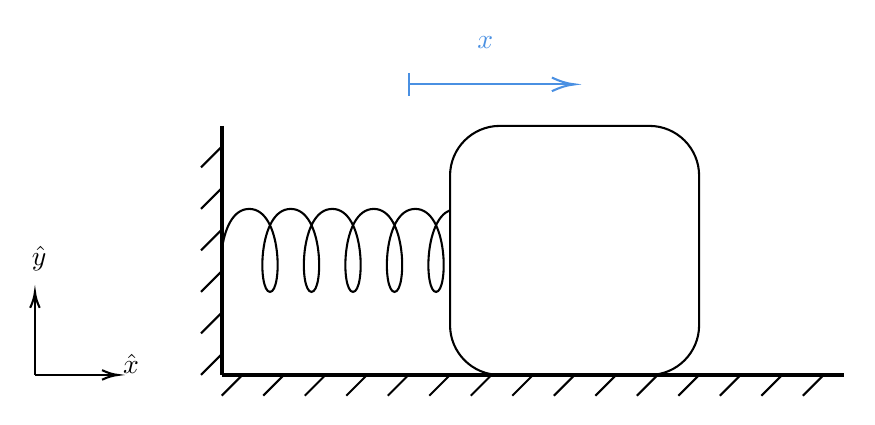
\begin{tikzpicture}[x=0.75pt,y=0.75pt,yscale=-1,xscale=1]
%uncomment if require: \path (0,300); %set diagram left start at 0, and has height of 300

%Rounded Rect [id:dp34438430167397516] 
\draw  [color={rgb, 255:red, 0; green, 0; blue, 0 }  ,draw opacity=1 ][fill={rgb, 255:red, 255; green, 255; blue, 255 }  ,fill opacity=1 ] (310,154) .. controls (310,140.75) and (320.75,130) .. (334,130) -- (406,130) .. controls (419.25,130) and (430,140.75) .. (430,154) -- (430,226) .. controls (430,239.25) and (419.25,250) .. (406,250) -- (334,250) .. controls (320.75,250) and (310,239.25) .. (310,226) -- cycle ;
%Straight Lines [id:da2744613466135113] 
\draw    (110,250) -- (110,212) ;
\draw [shift={(110,210)}, rotate = 90] [color={rgb, 255:red, 0; green, 0; blue, 0 }  ][line width=0.75]    (7.65,-2.3) .. controls (4.86,-0.97) and (2.31,-0.21) .. (0,0) .. controls (2.31,0.21) and (4.86,0.98) .. (7.65,2.3)   ;
%Straight Lines [id:da08431663295207847] 
\draw    (110,250) -- (148,250) ;
\draw [shift={(150,250)}, rotate = 180] [color={rgb, 255:red, 0; green, 0; blue, 0 }  ][line width=0.75]    (7.65,-2.3) .. controls (4.86,-0.97) and (2.31,-0.21) .. (0,0) .. controls (2.31,0.21) and (4.86,0.98) .. (7.65,2.3)   ;
%Shape: Spring [id:dp2050444045141704] 
\draw   (200,190) .. controls (201.25,180) and (205.25,170) .. (213.25,170) .. controls (229.25,170) and (229.25,210) .. (223.25,210) .. controls (217.25,210) and (217.25,170) .. (233.25,170) .. controls (249.25,170) and (249.25,210) .. (243.25,210) .. controls (237.25,210) and (237.25,170) .. (253.25,170) .. controls (269.25,170) and (269.25,210) .. (263.25,210) .. controls (257.25,210) and (257.25,170) .. (273.25,170) .. controls (289.25,170) and (289.25,210) .. (283.25,210) .. controls (277.25,210) and (277.25,170) .. (293.25,170) .. controls (309.25,170) and (309.25,210) .. (303.25,210) .. controls (297.69,210) and (297.28,175.62) .. (310,170.61) ;
%Straight Lines [id:da8109677911849542] 
\draw [line width=1.5]    (200,250) -- (500,250) ;
%Straight Lines [id:da9738860715008741] 
\draw [line width=1.5]    (200,130) -- (200,250) ;
%Straight Lines [id:da8479892294914445] 
\draw [color={rgb, 255:red, 74; green, 144; blue, 226 }  ,draw opacity=1 ]   (290,110) -- (368,110) ;
\draw [shift={(370,110)}, rotate = 180] [color={rgb, 255:red, 74; green, 144; blue, 226 }  ,draw opacity=1 ][line width=0.75]    (10.93,-3.29) .. controls (6.95,-1.4) and (3.31,-0.3) .. (0,0) .. controls (3.31,0.3) and (6.95,1.4) .. (10.93,3.29)   ;
\draw [shift={(290,110)}, rotate = 180] [color={rgb, 255:red, 74; green, 144; blue, 226 }  ,draw opacity=1 ][line width=0.75]    (0,5.59) -- (0,-5.59)   ;
%Straight Lines [id:da38778280879589844] 
\draw    (200,260) -- (210,250) ;
%Straight Lines [id:da13716831040628819] 
\draw    (220,260) -- (230,250) ;
%Straight Lines [id:da5435450145291132] 
\draw    (240,260) -- (250,250) ;
%Straight Lines [id:da6012450156738026] 
\draw    (260,260) -- (270,250) ;
%Straight Lines [id:da006204164316379712] 
\draw    (280,260) -- (290,250) ;
%Straight Lines [id:da6672054023307342] 
\draw    (300,260) -- (310,250) ;
%Straight Lines [id:da05532576658672206] 
\draw    (320,260) -- (330,250) ;
%Straight Lines [id:da713074642825677] 
\draw    (340,260) -- (350,250) ;
%Straight Lines [id:da054951797337481234] 
\draw    (360,260) -- (370,250) ;
%Straight Lines [id:da44290965384713543] 
\draw    (380,260) -- (390,250) ;
%Straight Lines [id:da1554621606788551] 
\draw    (400,260) -- (410,250) ;
%Straight Lines [id:da18496092525096441] 
\draw    (420,260) -- (430,250) ;
%Straight Lines [id:da9097830383289192] 
\draw    (440,260) -- (450,250) ;
%Straight Lines [id:da2668563479968923] 
\draw    (460,260) -- (470,250) ;
%Straight Lines [id:da6488797889553993] 
\draw    (480,260) -- (490,250) ;
%Straight Lines [id:da8070575578091496] 
\draw    (190,150) -- (200,140) ;
%Straight Lines [id:da3401604231163561] 
\draw    (190,170) -- (200,160) ;
%Straight Lines [id:da12031548793524682] 
\draw    (190,190) -- (200,180) ;
%Straight Lines [id:da3325006766252374] 
\draw    (190,210) -- (200,200) ;
%Straight Lines [id:da6789154128761035] 
\draw    (190,230) -- (200,220) ;
%Straight Lines [id:da23421921174832838] 
\draw    (190,250) -- (200,240) ;

% Text Node
\draw (151,238.4) node [anchor=north west][inner sep=0.75pt]    {$\hat{x}$};
% Text Node
\draw (107,186.4) node [anchor=north west][inner sep=0.75pt]    {$\hat{y}$};
% Text Node
\draw (327,90) node  [color={rgb, 255:red, 74; green, 144; blue, 226 }  ,opacity=1 ]  {$x$};

\end{tikzpicture}

    \caption{Mass-Spring System for Lagrangian}
    \label{fig:mass spring lagrange}
\end{figure}

We know the analytical form of the \gls{eom} from Newtonian Dynamics:
$$m\ddot{x}+kx=0$$
So, in essence, we are using the \gls{Lagrangian} \textit{a posteriori} to match this solution.

First, we will find the \gls{Lagrangian} of the system. The kinetic energy of the particle is given by the linear translation only (there is no rotational motion for a point particle), so we have $T=\frac{1}{2}m\dot{x}^2$. The potential energy is the energy of the spring, given as $U=\frac{1}{2}kx^2$. So, the \gls{Lagrangian} is:
$$L=\frac{1}{2}m\dot{x}^2-\frac{1}{2}kx^2$$
Now, applying \eqautoref{eq: Euler-Lagrange} in the $\hat{x}$-direction, as this is the only degree of freedom:
$$\frac{\partial L}{\partial x}-\frac{d}{dt}\frac{\partial L}{\partial \dot{x}}=0$$
Taking each term individually,
$$\frac{\partial L}{\partial x}=-kx$$
$$\frac{\partial L}{\partial \dot{x}}=m\dot{x}$$
$$\frac{d}{dt}\left(m\dot{x}\right)=m\ddot{x}$$
So, the \eqautoref{eq: Euler-Lagrange} equation gives us:
$$-kx-m\ddot{x}=0$$
A simple change of signs gives the exact same result as the Newtonian approach:
$$m\ddot{x}+kx=0$$
In this problem, we used a simple case where the dynamics were constrained along a single axis of motion. Before we move to a more complex problem, we will introduce the method by which \gls{Lagrangian} mechanics deals with these reference frames.
\section{Generalized Coordinates}
\color{red} Need to possibly reorganize some of this. Should explain why generalized coordinates are needed in the context of constraints and how they solve problems with coordinates being coupled.

\color{black}

We recall that in Newtonian mechanics, we describe reference frames for an object. We represent the position, velocity, and acceleration of a particle in terms of these coordinate systems as a tridimensional vector. 
Generally, we may write the $\vec{r}^{\ op}$  vector in a frame $a$ as:
$$x\hat{a}_1+y\hat{a}_2+z\hat{a}_3$$
Because any tridimensional set of coordinates that we choose that are linearly independent of each other will span $\mathbb{R}^3$, we can generalize this to any reference frame, $q$, where the terms of $a$ can be described by the terms of $q$:
$$x\left(q_1,q_2,q_3\right)+y\left(q_1,q_2,q_3\right)+z\left(q_1,q_2,q_3\right)$$
As a shorthand, we will write this full set of $q$, $\left(q_1,q_2,\cdots q_n\right)$, as $q_j$.

We can also generalize this to the velocity and the acceleration. The components of velocity can be written in terms of $q_j, \dot{q}_j$ and those for acceleration in terms of $q_j, \dot{q}_j, \ddot{q}_j$.  When we do Newtonian dynamics, we need to use the \gls{bke} to transform these quantities if they are not in an \gls{inertial frame}. Not so with the \gls{Lagrangian}! We are free to choose whatever $q$'s we want.

For a single particle, we can describe its position with the $q_j$ coordinates. When multiple particles are involved, we may need to increase this number of $q$ coordinates. As a very general statement, we can say for $N$ particles, we will need $n$ generalized coordinates in $q$. Expressed vectorially, given a particle of the $i^{\mathrm{th}}$ index:
$$\vec{r}^{\ oi}(q_j)$$
In other words, the position of an arbitrary particle is given in terms of $n$ generalized coordinates. 

The acceleration of the particles, when Newton's Laws are applied, are a function of the $q_j$ as well as their derivatives, $\dot{q}_j$. So, the evolution of the system exists in a $2n$-dimensional state space. However, we can use our previously mentioned \gls{Lagrangian} to circumvent the need for Newton's Law and the \gls{bke} in our derivation of the \gls{eom} using \textit{constraints} on the equation.

\subsection{Constraints}\label{sec:constaints}
Constraint equations are fundamental to \gls{Lagrangian} mechanics. In the previous section, I stated the need for $n$ generalized coordinates. To find a precise number for a given system, we turn our attention to constraints.

We can imagine constraints as a condition that restricts the motion of a body in some way. A body which has complete freedom to move translationally and rotate in any way is free. When a constraint is applied, this freedom is reduced. Often, we see these constraints denoted with either an equality or an inequality. These constraints, most often, are functions of the position, velocity, and/or time. We see constraints written most often in the form:
$$f(\vec{r},\vec{v},t)=0$$
The powerful thing about constraints in \gls{Lagrangian} mechanics is that we only need to know the way in which a particle is constrained, not the force or analytical description of this constraint. For complex problems, this can be especially useful.

\subsubsection{Holonomic Constraints}

To contextualize this, we take the example of a system of $N$ particles. For each particle, we need 3 values to define the position, so we need $3N$ generalized coordinates. 

\newglossaryentry{holonomic const}
{
    name=holonomic constraint,
    first = {\textit{holonomic constraint}},
    description={A constraint on a Lagrangian system which is a function of only the position of the particles},
    see={Lagrangian}
}

However, we often have constraints that reduce this number. Often, we see a problem that is planar or where the particles are connected in a \gls{rigid body}. These constraints will reduce the number of generalized coordinates needed. Here, we are only considering constraints on the positions of particles. Constraints on the positions of particles are known as \glspl{holonomic const}. 

A \gls{holonomic const} relates generalized coordinates to each other. In the commonly used notation, the \gls{holonomic const} is expressed in terms of the $q_j$'s as:
$$\Phi_k\left(q_j,t\right)=0, \ k=1\cdots K$$
or in terms of the position vectors:
$$f_k\left(\vec{r}^{\ op_1},\vec{r}^{\ op_2}\cdots \vec{r}^{\ op_N},t\right)=0$$
The number of \glspl{holonomic const}, $K$, will change the number of generalized coordinates as:
\begin{gather}\label{eq:dof}
\color{blue}\boxed{\color{black}\mathcal{M}=3N-K}\color{black}
\end{gather}
The quantity $\mathcal{M}$ is the number of \gls{dof}. However, this is the number of \gls{dof} for the whole system, which is why it can exceed 6 in some cases!

   \begin{example}[Particle on Path]
        Suppose we have a single particle that is constrained to motion along a path in the $xy$-plane. This path is given by $y=g(x)$. 
\begin{figure}[H]
    \centering



\tikzset{every picture/.style={line width=0.75pt}} %set default line width to 0.75pt        

\begin{tikzpicture}[x=0.75pt,y=0.75pt,yscale=-1,xscale=1]
%uncomment if require: \path (0,300); %set diagram left start at 0, and has height of 300

%Straight Lines [id:da4836354473889902] 
\draw    (280,200) -- (280,52) ;
\draw [shift={(280,50)}, rotate = 90] [color={rgb, 255:red, 0; green, 0; blue, 0 }  ][line width=0.75]    (7.65,-2.3) .. controls (4.86,-0.97) and (2.31,-0.21) .. (0,0) .. controls (2.31,0.21) and (4.86,0.98) .. (7.65,2.3)   ;
%Straight Lines [id:da02796272069122141] 
\draw    (280,200) -- (428,200) ;
\draw [shift={(430,200)}, rotate = 180] [color={rgb, 255:red, 0; green, 0; blue, 0 }  ][line width=0.75]    (7.65,-2.3) .. controls (4.86,-0.97) and (2.31,-0.21) .. (0,0) .. controls (2.31,0.21) and (4.86,0.98) .. (7.65,2.3)   ;
%Straight Lines [id:da7509100626039666] 
\draw    (280,200) -- (221.41,258.59) ;
\draw [shift={(220,260)}, rotate = 315] [color={rgb, 255:red, 0; green, 0; blue, 0 }  ][line width=0.75]    (7.65,-2.3) .. controls (4.86,-0.97) and (2.31,-0.21) .. (0,0) .. controls (2.31,0.21) and (4.86,0.98) .. (7.65,2.3)   ;
%Curve Lines [id:da26997678379551215] 
\draw [color={rgb, 255:red, 74; green, 144; blue, 226 }  ,draw opacity=1 ]   (210,180) .. controls (290.81,63.46) and (321.48,207.46) .. (410,90) ;
%Straight Lines [id:da09225730190804848] 
\draw [color={rgb, 255:red, 208; green, 2; blue, 27 }  ,draw opacity=1 ]   (280,200) -- (338.59,141.41) ;
\draw [shift={(340,140)}, rotate = 135] [color={rgb, 255:red, 208; green, 2; blue, 27 }  ,draw opacity=1 ][line width=0.75]    (10.93,-3.29) .. controls (6.95,-1.4) and (3.31,-0.3) .. (0,0) .. controls (3.31,0.3) and (6.95,1.4) .. (10.93,3.29)   ;
\draw [shift={(280,200)}, rotate = 315] [color={rgb, 255:red, 208; green, 2; blue, 27 }  ,draw opacity=1 ][fill={rgb, 255:red, 208; green, 2; blue, 27 }  ,fill opacity=1 ][line width=0.75]      (0, 0) circle [x radius= 3.35, y radius= 3.35]   ;
%Shape: Circle [id:dp7406066990608903] 
\draw  [fill={rgb, 255:red, 0; green, 0; blue, 0 }  ,fill opacity=1 ] (338.33,140) .. controls (338.33,139.08) and (339.08,138.33) .. (340,138.33) .. controls (340.92,138.33) and (341.67,139.08) .. (341.67,140) .. controls (341.67,140.92) and (340.92,141.67) .. (340,141.67) .. controls (339.08,141.67) and (338.33,140.92) .. (338.33,140) -- cycle ;

% Text Node
\draw (433,190.4) node [anchor=north west][inner sep=0.75pt]    {$x$};
% Text Node
\draw (277,22.4) node [anchor=north west][inner sep=0.75pt]    {$y$};
% Text Node
\draw (209,256.4) node [anchor=north west][inner sep=0.75pt]    {$z$};
% Text Node
\draw (282,203.4) node [anchor=north west][inner sep=0.75pt]    {$O$};
% Text Node
\draw (337,112.4) node [anchor=north west][inner sep=0.75pt]    {$P$};
% Text Node
\draw (420,72.4) node [anchor=north west][inner sep=0.75pt]  [color={rgb, 255:red, 74; green, 144; blue, 226 }  ,opacity=1 ]  {$y=g( x)$};
% Text Node
\draw (321,162.4) node [anchor=north west][inner sep=0.75pt]  [color={rgb, 255:red, 208; green, 2; blue, 27 }  ,opacity=1 ]  {$\vec{r}^{\ op}$};

\end{tikzpicture}

    \caption{Particle Moving on Constrained Path}
    \label{fig:constrainted path}
\end{figure}
We can select our generalized coordinates to be the same as the cartesian coordinates, so that:
\begin{gather}
    q_1=x\\q_2=y\\q_3=z
\end{gather}
With no other information, this is likely the best choice of generalized coordinates. However, we can start applying the constraints to simplify the equation. The first constraint is that the motion is confined to the $xy$-plane. Thus, 
$$q_3=z=0$$
Next, we have the path constraint which is given by $y=g(x)$. We can write this as a \glspl{holonomic const}:
\begin{gather}
    q_2-g(x)=0
\end{gather}
With these two constraints, we have reduced the number of degrees of freedom, $\mathcal{M}$, to 1. This makes sense intuitively, as the particle can only move along the path specified by the equation $g(x)$, therefore only having one degree of freedom.

In this example, we could describe that single degree of freedom with our coordinate, $q_1=x$.

The power of using generalized coordinates is that we could choose a coordinate that more easily defines this system. For example, our one coordinate could be the arc length along the path, $s$ defined from some starting point.
\end{example}

In general, these generalized coordinates do not even need to have units of length! We can select any parameters that are most convenient for defining the state, even those that are energies or fourier coefficients, so long as we can define a continuous derivative of that state and use the \gls{euler lagrange}.

\subsubsection{Rigid Body Constraints}\label{sec: rigid body constraints}
For most of the systems that we will deal with, including our rocket, we make the assumption that particles are rigidly attached to each other, meaning that there is no change in distance between particles. Using the notation of constraints described above, we will show how this is done for a two particle system, which can then naturally be extended with more particles.

Given two particles that are connected together by a massless rigid rod of length L, we have a constraint on the particles distance:
$$\left\Vert \vec{r}^{\ op_1}-\vec{r}^{\ op_2}\right\Vert=L$$
Written in the more standard notation:
$$f\left(\vec{r}^{\ op_1},\vec{r}^{\ op_2}\right)=\left\Vert \vec{r}^{\ op_1}-\vec{r}^{\ op_2}\right\Vert-L=0$$
So this constraint takes the 6-\gls{dof} for the two particles and reduces it to 5-\gls{dof}.

An example of the generalized coordinates describing this system would be the position of the first particle in Cartesian coordinates (giving 3 of the generalized coordinates, $x,y,z$, and the azimuthal and elevation angle, $\phi$ and $\theta$. The roll angle does not change the system in any measurable way, hence we only need 5 parameters to define a two particle system.

In the general case of $N$ particles composing a \gls{rigid body}, we have $3N$-\gls{dof} in a completely unconstrained system. However, we must constrain each pair of particles. An example of this for the 3 particle system in shown in \autoref{fig:rigid body 3 particle}.

\begin{figure}[ht]
    \centering
 

\tikzset{every picture/.style={line width=0.75pt}} %set default line width to 0.75pt        

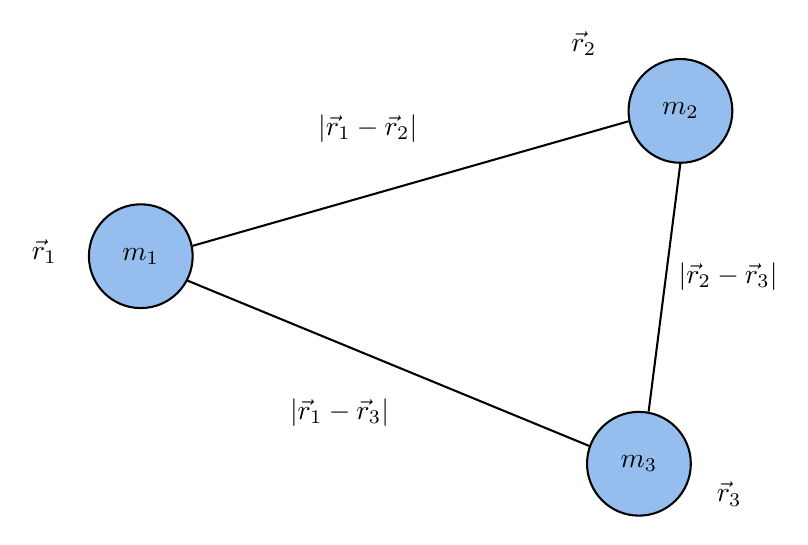
\begin{tikzpicture}[x=0.75pt,y=0.75pt,yscale=-1,xscale=1]
%uncomment if require: \path (0,300); %set diagram left start at 0, and has height of 300

%Shape: Circle [id:dp11919774335444377] 
\draw  [fill={rgb, 255:red, 74; green, 144; blue, 226 }  ,fill opacity=0.59 ] (120,135) .. controls (120,121.19) and (131.19,110) .. (145,110) .. controls (158.81,110) and (170,121.19) .. (170,135) .. controls (170,148.81) and (158.81,160) .. (145,160) .. controls (131.19,160) and (120,148.81) .. (120,135) -- cycle ;
%Shape: Circle [id:dp1512759538865308] 
\draw  [fill={rgb, 255:red, 74; green, 144; blue, 226 }  ,fill opacity=0.59 ] (360,235) .. controls (360,221.19) and (371.19,210) .. (385,210) .. controls (398.81,210) and (410,221.19) .. (410,235) .. controls (410,248.81) and (398.81,260) .. (385,260) .. controls (371.19,260) and (360,248.81) .. (360,235) -- cycle ;
%Shape: Circle [id:dp4443678325062712] 
\draw  [fill={rgb, 255:red, 74; green, 144; blue, 226 }  ,fill opacity=0.59 ] (380,65) .. controls (380,51.19) and (391.19,40) .. (405,40) .. controls (418.81,40) and (430,51.19) .. (430,65) .. controls (430,78.81) and (418.81,90) .. (405,90) .. controls (391.19,90) and (380,78.81) .. (380,65) -- cycle ;
%Straight Lines [id:da963502184755707] 
\draw    (170,130) -- (380,70) ;
%Straight Lines [id:da5114822387415651] 
\draw    (167.27,146.68) -- (361.67,226.68) ;
%Straight Lines [id:da3674207943033927] 
\draw    (405,90) -- (389.67,209.88) ;

% Text Node
\draw (145,135) node    {$m_{1}$};
% Text Node
\draw (385,235) node    {$m_{3}$};
% Text Node
\draw (405,65) node    {$m_{2}$};
% Text Node
\draw (91,125.4) node [anchor=north west][inner sep=0.75pt]    {$\vec{r}_{1}$};
% Text Node
\draw (421,242.4) node [anchor=north west][inner sep=0.75pt]    {$\vec{r}_{3}$};
% Text Node
\draw (351,25.4) node [anchor=north west][inner sep=0.75pt]    {$\vec{r}_{2}$};
% Text Node
\draw (229,65.4) node [anchor=north west][inner sep=0.75pt]    {$|\vec{r}_{1} -\vec{r}_{2} |$};
% Text Node
\draw (215.4,202.2) node [anchor=north west][inner sep=0.75pt]    {$|\vec{r}_{1} -\vec{r}_{3} |$};
% Text Node
\draw (402.6,136.6) node [anchor=north west][inner sep=0.75pt]    {$|\vec{r}_{2} -\vec{r}_{3} |$};

\end{tikzpicture}

    \caption{3 Particle Rigid Body}
    \label{fig:rigid body 3 particle}
\end{figure}

So, we have 3 constraint equations in a system with 9 particles. This gives a total of $3N-3=6$-\gls{dof}. When any additional particles are added, they must be fully constrained in all 3 translational degrees of freedom by constraints between $r_1$,$r_2$, and $r_3$. So, we always have constraints of the form $3N-3(N-2)$ for a \gls{rigid body}. This is why we always see a \gls{rigid body} displaying 6-\gls{dof}. We can then, of course, parametrize this in general coordinates with the cartesian coordinates and 3 angles.

\subsubsection{Minimal Set of Constraints}

\newglossaryentry{holonomic sys}
{
    name=holonomic system,
    first = {\textit{holonomic system}},
    description={A system that is entirely composed of holonomic constraints},
    see={holonomic const}
}
So far, we have only discussed holonomic constraints, those that are related to position or on the generalized parameters, and possibly have some relation in time. When a system is a \gls{holonomic sys}, that is, purely defined by \glspl{holonomic const}, it is always possible to find a set of $\mathcal{M}$ generalized parameters to describe the particle motion. In other words, the minimum number of parameters is equivalent to the number of degrees of freedom in the system.

That said, we often choose to use more parameters, particularly in the case of rotations. As we see in Volume II, we often find it more useful to use a non-minimal set of constraints to encode rotations to avoid singularities in the solution.

It is also common to see a non-minimal set of constraints used when the minimal set is cumbersome and does not give an intuitive feel to the problem. There is no strict requirement to use the minimal set of constraints for a problem, but you should be aware of the number of parameters required to describe the minimal set.
\subsubsection{Non-Holonomic Constraints}

\color{red} Discuss non integrability of non-holonomic constraints and the case of the rolling ball / ice skate.

\color{black}

\newglossaryentry{non holo const}
{
    name=non-holonomic constraint,
    first = {\textit{non-holonomic constraint}},
    description={A constraint that depends on more than the position of the particles in the system},
    see={holonomic const}
}
The other class of constraints are those constraints that are not merely a function of the generalized coordinates. These constraints, called \glspl{non holo const}, define the set of all constraints that depend on more than just the position of particles. This is a huge class of constraints, so we only cover specific cases here.

\newglossaryentry{gen vel}
{
    name=generalized velocity,
    first = {\textit{generalized velocity}},
    plural = {generalized velocities},
    firstplural = {\textit{generalized velocities}},
    description={A free direction of movement for a vehicle. These can be translational or rotational directions}
}

The most common among these, and where we will focus our attention here, is constraints on the time derivative of the generalized coordinates. These are called \glspl{gen vel}, denoted $\dot{q}_j$. Such an example of a constraint on \glspl{gen vel} is a roller skate. A roller stake only allows a velocity in the direction of the skate and restricts velocity along the direction normal to the roller stake.

One important thing about \glspl{non holo const} is that they do not reduce the number of parameters needed to define the system. Additionally, there is no general way to solve systems which have non-holonomic constraints. Later, we will look at a few cases which can be solved. For now, we will concern ourselves mostly with systems consisting of holonomic constraints.

It may seem that this limits us greatly, but in fact, this is not the case for most physics problems! When we are considering large systems, this may be quite limiting, but when considering small scale physics, such as atomic problems, we often find that \glspl{non holo const} are the exception, not the rule. Most systems are conservative and have constraints only on positions. As such, most of our modern theories can use these \glspl{Lagrangian}.

In the context of engineering problems, we can sometimes make derivations under the assumption of holonomic constraints and then use empirical data and correlations where needed to find suitable solutions (when friction or other factors are present).

\subsection{Lagrange's Equation in Generalized Coordinates}

The good thing about the \gls{Lagrangian} method is that it is invariant to changes in our coordinate system. Because the \gls{Lagrangian} is an equation of energy, and energy is independent of coordinate transformations, we can easily express the \gls{euler lagrange} in generalized coordinates with little hassle.\endnote{I note here that this explanation is not strictly correct, since our \gls{Lagrangian} does not have to be coordinate lengths. Instead, the configuration space has special properties that make it invariant to such transformations. Deriving the \gls{Lagrangian} from Hamilton's principle ensures that this is always true, which the intrepid reader may prove to themselves by studying differential geometry and Lagrangians on manifolds. Further information will be provided in \autoref{chap:lie theory} although we will not strictly cover this.} 

Using the generalized coordinates, the kinetic energy is a function of the generalized positions, velocities, and time. The potential is a function of the generalized position and time, so the \gls{Lagrangian} becomes:
$$L\equiv T-U=T(q_j,\dot{q}_j,t)-U(q_j,t)$$
Stated another way, the \gls{Lagrangian} is a function of the generalized positions, velocities, and time, as $L=L(q_j,\dot{q}_j,t)$. The \gls{euler lagrange} then becomes:
\begin{gather}\label{eq:Euler-Lagrange General}
\color{blue}\boxed{\color{black}\frac{\partial L}{\partial q_j}-\frac{d}{dt}\frac{\partial L}{\partial \dot{q}_j}=0,\quad j=1,2,\cdots M}\\
\mathrm{\color{blue}Generalized \ Euler-Lagrange \ Equations}
\end{gather}
Next we will show a problem where the rotational invariance and generalized coordinates proves especially useful in simplifying our derivation:
\section{Pendulum EOM Derivation}
\subsubsection{Problem Set-Up}
Suppose we have a pendulum of length L. The mass is rigidly attached to the pendulum. A reference frame $a$ that moves with the pendulum is shown in \autoref{fig:Pendulum}. The \gls{inertial frame} is also shown. The pendulum moves in only the $xy$ plane.
\begin{figure}[ht]

\centering

\tikzset{every picture/.style={line width=0.75pt}} %set default line width to 0.75pt        

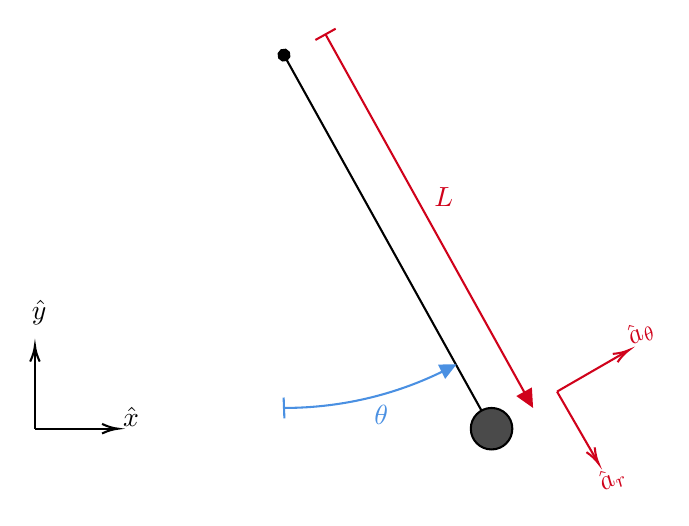
\begin{tikzpicture}[x=0.75pt,y=0.75pt,yscale=-1,xscale=1]
%uncomment if require: \path (0,300); %set diagram left start at 0, and has height of 300

%Straight Lines [id:da8354203825727349] 
\draw    (320,60) -- (420,240) ;
\draw [shift={(320,60)}, rotate = 60.95] [color={rgb, 255:red, 0; green, 0; blue, 0 }  ][fill={rgb, 255:red, 0; green, 0; blue, 0 }  ][line width=0.75]      (0, 0) circle [x radius= 2.68, y radius= 2.68]   ;
%Shape: Arc [id:dp31284247913451657] 
\draw  [draw opacity=0] (403.12,208.97) .. controls (378.54,222.36) and (350.19,230) .. (320,230) -- (320,65) -- cycle ; \draw [color={rgb, 255:red, 74; green, 144; blue, 226 }  ,draw opacity=1 ]   (400.15,210.55) .. controls (376.27,222.96) and (348.98,230) .. (320,230) ; \draw [shift={(320,230)}, rotate = 357.91] [color={rgb, 255:red, 74; green, 144; blue, 226 }  ,draw opacity=1 ][line width=0.75]    (0,5.03) -- (0,-5.03)   ; \draw [shift={(403.12,208.97)}, rotate = 153.52] [fill={rgb, 255:red, 74; green, 144; blue, 226 }  ,fill opacity=1 ][line width=0.08]  [draw opacity=0] (8.04,-3.86) -- (0,0) -- (8.04,3.86) -- cycle    ;
%Shape: Circle [id:dp5099783674397224] 
\draw  [color={rgb, 255:red, 0; green, 0; blue, 0 }  ,draw opacity=1 ][fill={rgb, 255:red, 74; green, 74; blue, 74 }  ,fill opacity=1 ] (410,240) .. controls (410,234.48) and (414.48,230) .. (420,230) .. controls (425.52,230) and (430,234.48) .. (430,240) .. controls (430,245.52) and (425.52,250) .. (420,250) .. controls (414.48,250) and (410,245.52) .. (410,240) -- cycle ;
%Straight Lines [id:da8713569921261672] 
\draw [color={rgb, 255:red, 208; green, 2; blue, 27 }  ,draw opacity=1 ]   (340,50) -- (438.54,227.38) ;
\draw [shift={(440,230)}, rotate = 240.95] [fill={rgb, 255:red, 208; green, 2; blue, 27 }  ,fill opacity=1 ][line width=0.08]  [draw opacity=0] (8.93,-4.29) -- (0,0) -- (8.93,4.29) -- cycle    ;
\draw [shift={(340,50)}, rotate = 240.95] [color={rgb, 255:red, 208; green, 2; blue, 27 }  ,draw opacity=1 ][line width=0.75]    (0,5.59) -- (0,-5.59)   ;
%Straight Lines [id:da9538559670922312] 
\draw    (200,240) -- (200,202) ;
\draw [shift={(200,200)}, rotate = 90] [color={rgb, 255:red, 0; green, 0; blue, 0 }  ][line width=0.75]    (7.65,-2.3) .. controls (4.86,-0.97) and (2.31,-0.21) .. (0,0) .. controls (2.31,0.21) and (4.86,0.98) .. (7.65,2.3)   ;
%Straight Lines [id:da3275390122881038] 
\draw    (200,240) -- (238,240) ;
\draw [shift={(240,240)}, rotate = 180] [color={rgb, 255:red, 0; green, 0; blue, 0 }  ][line width=0.75]    (7.65,-2.3) .. controls (4.86,-0.97) and (2.31,-0.21) .. (0,0) .. controls (2.31,0.21) and (4.86,0.98) .. (7.65,2.3)   ;
%Straight Lines [id:da24072013587186947] 
\draw [color={rgb, 255:red, 208; green, 2; blue, 27 }  ,draw opacity=1 ]   (451.54,222.12) -- (470.54,255.03) ;
\draw [shift={(471.54,256.77)}, rotate = 240] [color={rgb, 255:red, 208; green, 2; blue, 27 }  ,draw opacity=1 ][line width=0.75]    (7.65,-2.3) .. controls (4.86,-0.97) and (2.31,-0.21) .. (0,0) .. controls (2.31,0.21) and (4.86,0.98) .. (7.65,2.3)   ;
%Straight Lines [id:da7099456662568205] 
\draw [color={rgb, 255:red, 208; green, 2; blue, 27 }  ,draw opacity=1 ]   (451.54,222.12) -- (484.45,203.12) ;
\draw [shift={(486.18,202.12)}, rotate = 150] [color={rgb, 255:red, 208; green, 2; blue, 27 }  ,draw opacity=1 ][line width=0.75]    (7.65,-2.3) .. controls (4.86,-0.97) and (2.31,-0.21) .. (0,0) .. controls (2.31,0.21) and (4.86,0.98) .. (7.65,2.3)   ;


% Text Node
\draw (362,227.4) node [anchor=north west][inner sep=0.75pt]  [color={rgb, 255:red, 74; green, 144; blue, 226 }  ,opacity=1 ]  {$\theta $};
% Text Node
\draw (391,122.4) node [anchor=north west][inner sep=0.75pt]  [color={rgb, 255:red, 208; green, 2; blue, 27 }  ,opacity=1 ]  {$L$};
% Text Node
\draw (241,228.4) node [anchor=north west][inner sep=0.75pt]    {$\hat{x}$};
% Text Node
\draw (197,176.4) node [anchor=north west][inner sep=0.75pt]    {$\hat{y}$};
% Text Node
\draw (481.25,191.58) node [anchor=north west][inner sep=0.75pt]  [color={rgb, 255:red, 208; green, 2; blue, 27 }  ,opacity=1 ,rotate=-330]  {$\hat{a}_{\theta }$};
% Text Node
\draw (467.54,261.84) node [anchor=north west][inner sep=0.75pt]  [color={rgb, 255:red, 208; green, 2; blue, 27 }  ,opacity=1 ,rotate=-330]  {$\hat{a}_{r}$};

\end{tikzpicture}

    \caption{Pendulum Set-Up}
    \label{fig:Pendulum}
\end{figure}
Our goal here is to approach the problem in several different ways to gain insight into the benefits and drawbacks of each method in a practical setting.

\subsubsection{Newtonian Approach}
You have likely seen the Newtonian approach many times, but we show it here for completeness and to contrast the approach with the \gls{Lagrangian} more directly. 

In the Newtonian Approach to deriving EOM's, we always start with the forces governing the system. In this case, we have two forces. The gravitational force, $mg$, acts in the $-\hat{y}$-direction and the tension force acts in the $-\hat{a}_r$-direction. From the constraint on length, the acceleration in the $\hat{a}_r$ must be zero. Thus, the component of gravity in the $\hat{a}_r$ direction must equal the tension.

We express the gravity in the $a$-frame to find this:
$$\hat{y}=-\cos\theta\hat{a}_r+\sin\theta \hat{a}_\theta$$
So, by balancing the forces in the $\hat{a}_r$-direction:
$$m{\ddot{a}}_r=mg\cos\theta \hat{a}_r-\vec{F}_T$$
In the $\hat{a}_\theta$-direction, we have unconstrained motion, so $\sum\vec{F}=m\vec{a}$. Our force equation is thus: 
$$F=-mg\sin\theta\hat{a}_{\theta}$$
Next, we need to find our acceleration in the \gls{inertial frame} using the \gls{bke} to solve the RHS of the force balance. Starting with the position vector:
$$\vec{r}^{\ op}=L\hat{a}_r$$
We can apply the \gls{bke} to find our inertial velocity:
$${}^i\vec{v}^p={}^a\frac{d}{dt}\vec{r}^{\ op}+{}^i\omega^a\times\vec{r}^{\ op}$$
Plugging in appropriate quantities:
$${}^i\vec{v}^p={}^a\frac{d}{dt}(L\hat{a}_r)+\dot{\theta}\hat{a}_3\times(L\hat{a}_r)$$
$${}^i\vec{v}^p=\dot{\theta}L\hat{a}_\theta$$
We do this again to find the inertial acceleration:
$${}^i\vec{a}^p={}^a\frac{d}{dt}{}^i\vec{v}^p+{}^i\omega^a\times{}^i\vec{v}^p$$
$${}^i\vec{a}^p={}^a\frac{d}{dt}{}\dot{\theta}L\hat{a}_\theta+\dot{\theta}\hat{a}_3\times\dot{\theta}L\hat{a}_\theta$$
$${}^i\vec{a}^p=\ddot{\theta}L\hat{a}_\theta-\dot{\theta}^2L\hat{a}_r$$
Now, we equate the forces in each direction:
$$-mg\sin\theta\hat{a}_\theta=\ddot{\theta}L\hat{a}_\theta$$
Rearranging, we arrive at our \gls{eom}:
$$\ddot{\theta}+\frac{g}{L}\sin\theta=0$$
\subsubsection{Lagrangian Approach}
In the \gls{Lagrangian} approach, we will start by defining our constraints and coordinates. Some preliminary analysis shows that using polar coordinates for this problem will be useful. If we do not recognize this, we can always convert later (a distinct advantage of the \gls{Lagrangian} approach, since it is coordinate frame invariant). Here we will choose a cylindrical coordinate systsem:
\begin{gather}
    q_1=r\\q_2=\theta\\q_3=z
\end{gather}
Next, we define constraints. Since there is no motion in the z-axis:
$$z=0$$
And the constraint on the length gives us:
$$q_1-L=0$$
So, we have 1 \gls{dof} from \eqautoref{eq:dof}. Since both $z$ and $r$ are constrained, we can express our \gls{eom} in terms of one generalized coordinate, $\theta$.

Next, we define the \gls{Lagrangian}. Knowing that the linear velocity of the particle is $\dot{\theta}L$, we get:
$$T=\frac{1}{2}m\dot{\theta}^2L^2$$
For the potential, we choose the origin as our reference, giving us:
$$U=-mgy$$
And a coordinate transformation into polar using $y=r\cos\theta$ yields:
$$U=-mgL\cos\theta$$
This gives the \gls{Lagrangian}:
$$L=\frac{1}{2}m\dot{\theta}^2L^2+mgL\cos\theta$$
Applying the Euler-Lagrange formula for generalized coordinates, \eqautoref{eq:Euler-Lagrange General} on the single generalized coordinate:
\begin{gather}
    \frac{\partial L}{\partial \theta}=-mgL\sin\theta\\
    \frac{\partial L}{\partial \dot{\theta}}=mL^2\dot{\theta}\\
    \frac{d}{dt}\left(mL^2\dot{\theta}\right)=mL^2\ddot{\theta}
\end{gather}
So, the final system is:
$$-mgL\cos\theta -mL^2\ddot{\theta}=0$$
With some rearrangement:
$$\ddot{\theta}+\frac{g}{L}\sin\theta=0$$
We notice that with the \gls{Lagrangian} approach, we did not need to have an understanding of the vector directions, frame translations, or \gls{bke} to find our \gls{eom}. This, in addition to the flexibility of the generalized coordinates, is the real power of this approach.

\subsubsection{Kinetic Energy Generalization}
In the previous two examples that we explored, the functions for $T$ and $U$ were quite simple because the transformations from the generalized coordinates were quite simple and could be understood from intuition. In the case that they are not as simple, we would previously have to use \gls{bke} to find transformations or employ some other method. It would be useful if we had a general formula to express $T$ and $U$ in the generalized coordinates. We know that the kinetic energy is simply the following:
$$T=\frac{1}{2}\sum_im_i{v_i}^2$$
We can more explicitly define $v_i$ to be $\dot{r}_i$, with $r$ being the vector in cartesian coordinates. The kinetic energy in terms of $\dot{r}$ is thus:
$$T=\frac{1}{2}\sum_im_i(\dot{r}_i\cdot\dot{r}_i)$$
As we have shown before, $r_i$ can generally be represented in terms of the generalized positions, $q_j$:
$$r_i=r_i(q_j)$$
As a result, $\dot{r}$ can be expressed in terms of the generalized positions and velocities using the chain rule (it is worth doing this derivation yourself!):
$$\dot{r}=\frac{dr}{dt}=\sum_k{\frac{\partial r_i}{\partial q_k}\dot{q}_k+\frac{\partial r_i}{\partial t}}$$
Combining these two formulas, it is quite easy to see that we have the following for a general formula of the kinetic energy which converts between $r$ and the generalized coordinates\endnote{See \cite{goldstein_classical_2008} Chapter 1.6 for more information on this derivation} :
$$T=\frac{1}{2}\sum_im_i\left(\sum_j\frac{\partial\vec{r}_i}{\partial q_j}\dot{q}_j+\frac{\partial \vec{r}_i}{\partial t}\right)^2$$

\begin{example}[Free Particle in Polar Coordinates]
We can show this equation in work with a simple example of a single free particle. We express the motion in polar coordinates in order to showcase the use of the formula. We need only know the transformations between the coordinate systems.

We define the two cartesian coordinates of interest $x$ and $y$ such that $r=\sqrt{x^2+y^2}$. The two \gls{Lagrangian} coordinates are $r$ and $\theta$ since we have assumed polar coordinates. We are free, of course, to choose anything. The one fact we need to complete the derivation is that 
\begin{gather}
    x=r\cos\theta\\
    y=r\sin\theta
\end{gather}
Of course, for a more general problem, there are methods to derive these relations if they are more complex, such as the Jacobian matrix.

Since we are only considering a single particle in this example, the sum over $i$ for different masses need not be considered. We thus have:
$$T=\frac{1}{2}m\left[\left(\frac{\partial r_1}{\partial r}\dot{r}+\frac{\partial r_1}{\partial t}\right)^2+\left(\frac{\partial r_1}{\partial \theta}\dot{\theta}+\frac{\partial r_1}{\partial t}\right)^2\right]$$
We can quite easily eliminate the term $\frac{\partial r}{\partial t}$, since nothing has explicit dependence on time in our problem. From here, the problem is simply `bookkeeping' to ensure that all of the partial derivatives are performed properly. Expressing $r_1 = (r\cos\theta,r\sin\theta)$:
$$\begin{array}{l}
\dfrac{\partial}{\partial r}r_1=(\cos\theta,\sin\theta)\\
    \dfrac{\partial}{\partial \theta}r_1=(-r\sin\theta,r\cos\theta)
\end{array}$$
Plugging back in, we have:
$$T=\frac{1}{2}m\left[\left(\dot{r}\cos\theta-r\sin\theta\dot{\theta}\right)^2+\left(\dot{r}\sin\theta-r\cos\theta\dot{\theta}\right)^2\right]$$
Upon computation of the cross terms, we find that they cancel and are left with:
$$T=\frac{1}{2}m\left[\dot{r}^2+r^2\dot{\theta}^2\right]$$
Which matches the Newtonian result and is generally applicable to many cases. More of this approach will be seen later in the case of the inverted pendulum.
\end{example}

\section{Cyclic Coordinates and Conservation}
The \gls{Lagrangian} formulation of mechanics can give us some special insight into the quantities of a problem that are conserved. This is, once again, one of the distinct advantages over the Newtonian approach. In the Newtonian scheme, we can learn to recognize when systems will have conserved quantities, but there is no satisfactory analysis we can perform beforehand to ensure this. 

With \gls{Lagrangian} mechanics, we can employ several methods to understand conservation. The ideas discussed here are more deeply tied to Noether's Theorem, the mathematical background of which is more heavily discussed in \autoref{Noether's Theorem}.

We can understand conservation of linear momentum in a system quite easily in the case of the \gls{Lagrangian}. In fact, we have already seen it in some of our examples.

\begin{example}{Rolling Wheel}
Let us consider a system consisting of a wheel which is rolling without slipping along a level surface, as shown in \autoref{fig:roll wheel}:
\begin{figure}[H]
    \centering

\tikzset{every picture/.style={line width=0.75pt}} %set default line width to 0.75pt        

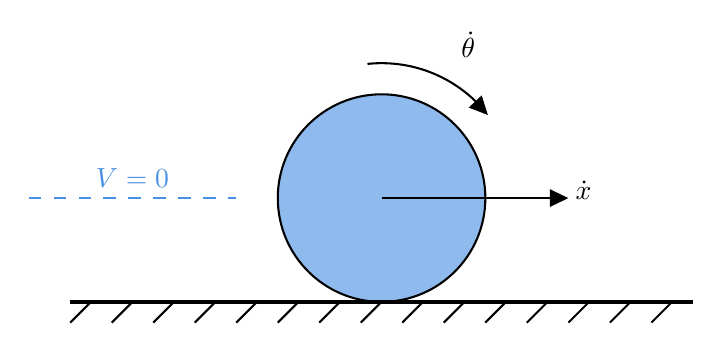
\begin{tikzpicture}[x=0.75pt,y=0.75pt,yscale=-1,xscale=1]
%uncomment if require: \path (0,300); %set diagram left start at 0, and has height of 300

%Shape: Circle [id:dp5489222813863226] 
\draw  [fill={rgb, 255:red, 74; green, 144; blue, 226 }  ,fill opacity=0.62 ] (280,160) .. controls (280,132.39) and (302.39,110) .. (330,110) .. controls (357.61,110) and (380,132.39) .. (380,160) .. controls (380,187.61) and (357.61,210) .. (330,210) .. controls (302.39,210) and (280,187.61) .. (280,160) -- cycle ;
%Straight Lines [id:da04211062143200128] 
\draw [line width=1.5]    (180,210) -- (480,210) ;
%Straight Lines [id:da6500950261729116] 
\draw    (180,220) -- (190,210) ;
%Straight Lines [id:da6134937051620686] 
\draw    (200,220) -- (210,210) ;
%Straight Lines [id:da3689063615429048] 
\draw    (220,220) -- (230,210) ;
%Straight Lines [id:da5567221191324185] 
\draw    (240,220) -- (250,210) ;
%Straight Lines [id:da3331253564911133] 
\draw    (260,220) -- (270,210) ;
%Straight Lines [id:da14247859045384603] 
\draw    (280,220) -- (290,210) ;
%Straight Lines [id:da8370679307995611] 
\draw    (300,220) -- (310,210) ;
%Straight Lines [id:da711076493058232] 
\draw    (320,220) -- (330,210) ;
%Straight Lines [id:da5761077435987036] 
\draw    (340,220) -- (350,210) ;
%Straight Lines [id:da8146033682447109] 
\draw    (360,220) -- (370,210) ;
%Straight Lines [id:da3200839493652361] 
\draw    (380,220) -- (390,210) ;
%Straight Lines [id:da9028378067670185] 
\draw    (400,220) -- (410,210) ;
%Straight Lines [id:da2490962151726679] 
\draw    (420,220) -- (430,210) ;
%Straight Lines [id:da9030762040565409] 
\draw    (440,220) -- (450,210) ;
%Straight Lines [id:da15742997205460696] 
\draw    (460,220) -- (470,210) ;
%Straight Lines [id:da8395154480795631] 
\draw    (330,160) -- (417,160) ;
\draw [shift={(420,160)}, rotate = 180] [fill={rgb, 255:red, 0; green, 0; blue, 0 }  ][line width=0.08]  [draw opacity=0] (8.93,-4.29) -- (0,0) -- (8.93,4.29) -- cycle    ;
%Shape: Arc [id:dp6538226703220662] 
\draw  [draw opacity=0] (323.21,95.35) .. controls (325.44,95.12) and (327.71,95) .. (330,95) .. controls (350.8,95) and (369.33,104.77) .. (381.22,119.98) -- (330,160) -- cycle ; \draw    (323.21,95.35) .. controls (325.44,95.12) and (327.71,95) .. (330,95) .. controls (349.76,95) and (367.47,103.82) .. (379.39,117.74) ; \draw [shift={(381.22,119.98)}, rotate = 226.89] [fill={rgb, 255:red, 0; green, 0; blue, 0 }  ][line width=0.08]  [draw opacity=0] (8.93,-4.29) -- (0,0) -- (8.93,4.29) -- cycle    ; 
%Straight Lines [id:da9468521926710415] 
\draw [color={rgb, 255:red, 74; green, 144; blue, 226 }  ,draw opacity=1 ] [dash pattern={on 4.5pt off 4.5pt}]  (160,160) -- (260,160) ;

% Text Node
\draw (422,150.4) node [anchor=north west][inner sep=0.75pt]    {$\dot{x}$};
% Text Node
\draw (367,78.4) node [anchor=north west][inner sep=0.75pt]    {$\dot{\theta }$};
% Text Node
\draw (210,156.6) node [anchor=south] [inner sep=0.75pt]  [color={rgb, 255:red, 74; green, 144; blue, 226 }  ,opacity=1 ]  {$V=0$};

\end{tikzpicture}
    \caption{Rolling Wheel}
    \label{fig:roll wheel}
\end{figure}
The \gls{Lagrangian} for such a system is quite simple. Since the center of mass is aligned with the zero potential height, we can disregard $V$ and only consider the kinetic energy $T$. The kinetic energy is given as the combination of the rotational and translational motions:
$$L=T=\frac{1}{2}\left(m\dot{x}^2+I\dot{\theta}^2\right)$$
The value of $I$ will change depending on the mass distribution of the rolling object, but the exact value of $I$ is unimportant here.

We can now consider the Euler-Lagrange equation for each coordinate, taking $x$ first:
$$\frac{d}{dt}\left(\frac{\partial L}{\partial \dot{x}}\right)=\frac{\partial L}{\partial x}$$
The partial with respect to $x$ yields $0$ since the coordinate $x$ appears nowhere in the \gls{Lagrangian}. When this is the case -- that a variable does not appear directly in the \gls{Lagrangian} -- it is \textit{cyclic}. Whenever a coordinate is cyclic, its partial derivative is 0.

Thus, we can see that $\frac{d}{dt}\left(\frac{\partial L}{\partial \dot{x}}\right)=0$ and thus $\frac{\partial L}{\partial \dot{x}}=\mathrm{const.}$ The result of this is that the linear momentum of the system is conserved, since it is constant! This result is one possible result of Noether's Theorem -- that linear momentum is conserved when the \gls{Lagrangian} is independent of position. \endnote{More precisely, the theorem states that the \gls{Lagrangian} must be invariant under a continuous transformation, but this is touched on much more in \autoref{Noether's Theorem}}.

We can apply the same reasoning to the $\theta$ component, and we see that:
$$I\dot{\theta}=\mathrm{const.}$$
Which is the statement that the angular momentum of the system is conserved.
\end{example}

Although a more general discussion of these topics is saved for later, the concept of cyclic coordinates and conserved quantities will be used throughout the proceeding text, and it is important to keep these concepts in mind!

\section{Generalized Forces}
The next thing that we need to consider in our journey through \gls{Lagrangian} mechanics are \textit{generalized  forces}. In analogy to the other generalized quantities, generalized forces derive from the standard definitions of forces and can then be applied to other coordinate systems and more complex situations.


\subsection{D'Alembert's Principle}

\section{Lagrange Multipliers}
In our discussion of constraints, there was a discussion between holonomic and non-holonomic constraints. As we further progress our knowledge, it should be stated that the key difference between these two in actually solving problems is that holonomic constraints are \textit{integrable}, while non-holonomic constraints generally are not.

Sometimes, this integrability can be tricky, though. We need to apply Lagrange multipliers in some instances to be able to integrate.

\section{Lagrangian Rigid Body Dynamics}

In Volume I, we explored the Newtonian method of deriving the Euler rotation equations using the \gls{bke}. Here, we present an alternative derivation that utilizes the \gls{Lagrangian} approach and is ultimately a more fundamental derivation.

We showed earlier in \autoref{sec: rigid body constraints} that we can describe a \gls{rigid body} system with 6 generalized parameters, three of which are angles.
\subsection{Torque Free Equations}
In the case of no applied torque, the derivations of \glspl{Euler Equation} become surprisingly simple. We can assume that the change in height of the \gls{rigid body} is irrelevant for pure rotation, so the \gls{Lagrangian} is simply the kinetic energy of the object. We can suppose that we are also in a coordinate system where the translational kinetic energy is 0. This gives:
\begin{equation}\label{eq:rigid body KE}
L=\frac{1}{2}I\omega^2
\end{equation}
We can select our generalized coordinates as the three Euler angles, $\psi$, $\theta$, and $\phi$ (see Volume II for more info).

Selecting the generalized coordinate, $\psi$, as an example, the Euler-Lagrange equation gives:
$$\frac{\partial L}{\partial \psi}-\frac{d}{dt}\frac{\partial L}{\partial \dot{\psi}}=0$$
Using the derivation of the components of angular velocity using Euler Angles, we have:
\begin{gather}
\omega_1=\dot{\phi}\sin\theta\sin\psi+\dot{\theta}\cos\psi\\
    \omega_2=\dot{\phi}\sin\theta\cos\psi-\dot{\theta}\sin\psi\\
    \omega_3=\dot{\phi}\cos\theta+\dot{\psi}
\end{gather}
So, we can also express our \gls{Lagrangian} in terms of the angular acceleration:
$$\frac{\partial L}{\partial \omega_i}\frac{\partial \omega_i}{\partial \psi}-\frac{d}{dt}\frac{\partial L}{\partial \omega_i}\frac{\partial \omega_i}{\partial \dot{\psi}}=0$$
At this point, the derivation is simply a matter of 'plug and chug'. Calculating the derivatives with respect to $\psi$:
\begin{gather}
    \frac{\partial \omega_1}{\partial \psi}=-\dot{\phi}\sin\theta\cos\psi-\dot{\theta}\sin\psi\\
    \frac{\partial \omega_2}{\partial \psi}=-\dot{\phi}\sin\theta\sin\psi-\dot{\theta}\cos\psi\\
    \frac{\partial \omega_3}{\partial \psi}=0
\end{gather}
We notice here that $\frac{\partial \omega_1}{\partial \psi}=\omega_2$ and $\frac{\partial \omega_2}{\partial \psi}=-\omega_1$. Next, taking our derivatives with respect to $\dot{\psi}$:
\begin{gather}
    \frac{\partial \omega_1}{\partial \dot{\psi}}=0\\
    \frac{\partial \omega_2}{\partial \dot{\psi}}=0\\
    \frac{\partial \omega_3}{\partial \dot{\psi}}=1
\end{gather}
Last, we can make a substitution for the $\frac{\partial L}{\partial \omega_i}$ term by taking a derivative of the kinetic energy \eqautoref{eq:rigid body KE}:
$$\frac{\partial L}{\partial \omega_i}=I_i\omega_i$$
Plugging everything into the Euler-Lagrange formula, we have:
$$I_1\omega_1\omega_2-I_2\omega_1\omega_2-\frac{d}{dt}I_3\omega_3=0$$
Some simplification yields:
$$\left(I_1-I_2\right)\omega_1\omega_2=I_3\dot{\omega_3}$$
We can perform the analogous analysis for the other axes, yielding the full set of torque free \gls{rigid body} equations:
\begin{gather}
\color{blue}\boxed{
\begin{array}{ll}
\color{black}
\left(I_y-I_z\right)\omega_y\omega_z=I_x\dot{\omega_x}
     &\\
     \color{black}\left(I_z-I_x\right)\omega_x\omega_z=I_y\dot{\omega_y}
     &\\
     \color{black}\left(I_x-I_y\right)\omega_x\omega_y=I_z\dot{\omega_z}
\end{array}}\\
\color{blue}
\mathrm{Torque-Free \ Rotations}
\end{gather}
\subsection{Forced Euler Rigid Body Dynamics}

\section{From Quantum to Lagrangian Mechanics}
Taking inspiration from \autoref{sec: connection to quantum} where I showed the connection between the principle of least time and the quantum formulation of the phenomenon, can we find a similar underlying principle for all of classical mechanics?

Luckily, we can! This section will tackle the formalization of the topics discussed in \autoref{sec: connection to quantum} and extend them to the case far beyond the paths of light rays. A great video explanation, much of which is discussed here, is found in \cite{physics_with_elliot_how_2023}.

Having started our study of classical mechanics, we now know that the same underlying principle dictates the motion of both light and classical behaviors -- the minimization of action. 

For light, we could quite intuitively understand how this principle emerges using the phase of the light. For typical particles and rigid bodies, we can't measure a phase. Therefore, we need an approach that encompasses both phenomenon.


 \section{A Vector Calculus Approach to Hamilton's Principle}

 We have so far seen that Hamilton's principle is useful for solving these problems. Now, with our background for generalized coordinates built up, we can explore a derivation of the action which will explain the presence of the $T-U$ term and the $T+U$ term in the \gls{Hamiltonian}.

The approach described here comes mainly from the work in \cite{carcassi_geometric_2023}. I have simplified some of the details of this approach to make this section more simple for the reader, but I recommend reading this paper for a deeper understanding of the subject.
 

\section{Key Ideas}
\begin{enumerate}
    \item We can find the \gls{eom} of a system using either the Newtonian approach or the \gls{Lagrangian} approach, and it is often easier to find an \gls{eom} using the \gls{Lagrangian} for a \gls{conservative} system.
    \item The \gls{Lagrangian} is scalar, so it is invariant to coordinate transforms. This means we can choose any variables we want for our generalized coordinates when performing derivations.
    \item The methodology of Newtonian mechanics and \gls{Lagrangian} mechanics are fundementally different. Newtonian mechanics deals with the influence of external \glspl{action} (forces), while \gls{Lagrangian} Mechanics emphasizes the internal state of the system.
    \item %add Hamiltonian v. Lagrangian
\end{enumerate}
\section{Further Reading}
The first section borrows from the derivations of Chapter 6 and 7 of  \cite{thornton_classical_nodate} and Chapter 5 of  \cite{cline_variational_2017}. These sources are a good first introduction to the subject with simple mathematics.

The most useful book for further study (and one I have read with much scrutiny in constructing these chapters), is \cite{goldstein_classical_2008}. This book is most definitely a graduate level treatment of the subject, but is extremely thorough and goes deep into many topics which have not been discussed here for the sake of brevity. Much knowledge is expected of the reader, so I find this book best for further study only after consulting some other sources first.

There are an abundance of video sources for classical mechanics. A good conceptual video overview of this topic can be found at \cite{veritasium_closest_2024}. This video contains little math, but is quite good for understanding the reasoning behind the formulation. I can personally recommend the video series at \cite{ross_lagranges_nodate}, which covers this material in a more suitable manner to engineering contexts and is quite easy to follow along with.

\section{Practice Problems}
\begin{enumerate}
    \item Arthur keeps finding bugs on the apples that he is feeding his horse. Arthur heard that you have been learning about generalized coordinates. He wants a way to describe the position of the bugs on his apples using a minimal set of coordinates.

Find a suitable set of generalized coordinates to describe this system. Write out any equations of constraints of the system. \textit{Hint: A apple is topologically similar to a sphere!}

\item  Th\'eoden, king of the Rohirrim, is riding his armies north through the Emyn Muil. His horse, Snowmane, trips on a small rock and Th\'eoden begins to lose his balance.

You can model Th\'eoden as a mass on the end of a massless rod and his horse as a cart constrained to motion along the $\hat{x}$-axis. The angle of Th\'eoden from the vertical is denoted as $\theta$. Derive the \gls{eom} of the system using energy methods. The set-up is shown in \autoref{fig:Inverted Pendulum}.
\begin{figure}[ht]
    \centering

\tikzset{every picture/.style={line width=0.75pt}} %set default line width to 0.75pt        

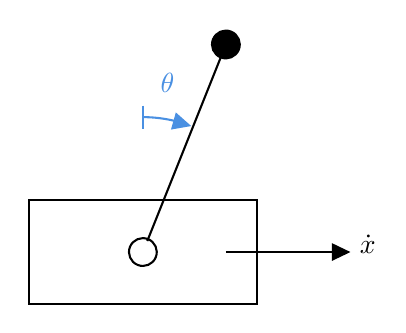
\begin{tikzpicture}[x=0.75pt,y=0.75pt,yscale=-1,xscale=1]
%uncomment if require: \path (0,300); %set diagram left start at 0, and has height of 300

%Shape: Rectangle [id:dp1823165404229382] 
\draw   (270,160) -- (380,160) -- (380,210) -- (270,210) -- cycle ;
%Straight Lines [id:da7877170508964265] 
\draw    (365,85) -- (327.12,179.71) ;
\draw [shift={(325,185)}, rotate = 111.8] [color={rgb, 255:red, 0; green, 0; blue, 0 }  ][line width=0.75]      (0, 0) circle [x radius= 6.7, y radius= 6.7]   ;
\draw [shift={(365,85)}, rotate = 111.8] [color={rgb, 255:red, 0; green, 0; blue, 0 }  ][fill={rgb, 255:red, 0; green, 0; blue, 0 }  ][line width=0.75]      (0, 0) circle [x radius= 6.7, y radius= 6.7]   ;
%Straight Lines [id:da5998055377665403] 
\draw    (365,185) -- (422,185) ;
\draw [shift={(425,185)}, rotate = 180] [fill={rgb, 255:red, 0; green, 0; blue, 0 }  ][line width=0.08]  [draw opacity=0] (8.93,-4.29) -- (0,0) -- (8.93,4.29) -- cycle    ;
%Shape: Arc [id:dp2580429075144265] 
\draw  [draw opacity=0] (325,120) .. controls (325,120) and (325,120) .. (325,120) .. controls (325,120) and (325,120) .. (325,120) .. controls (333.21,120) and (341.07,121.52) .. (348.3,124.3) -- (325,185) -- cycle ; \draw [color={rgb, 255:red, 74; green, 144; blue, 226 }  ,draw opacity=1 ]   (325,120) .. controls (325,120) and (325,120) .. (325,120) .. controls (325,120) and (325,120) .. (325,120) .. controls (332.18,120) and (339.1,121.17) .. (345.56,123.32) ; \draw [shift={(348.3,124.3)}, rotate = 195.83] [fill={rgb, 255:red, 74; green, 144; blue, 226 }  ,fill opacity=1 ][line width=0.08]  [draw opacity=0] (8.93,-4.29) -- (0,0) -- (8.93,4.29) -- cycle    ; \draw [shift={(325,120)}, rotate = 180] [color={rgb, 255:red, 74; green, 144; blue, 226 }  ,draw opacity=1 ][line width=0.75]    (0,5.59) -- (0,-5.59)   ;

% Text Node
\draw (428,175.4) node [anchor=north west][inner sep=0.75pt]    {$\dot{x}$};
% Text Node
\draw (332,97.4) node [anchor=north west][inner sep=0.75pt]  [color={rgb, 255:red, 74; green, 144; blue, 226 }  ,opacity=1 ]  {$\theta $};


\end{tikzpicture}

    \caption{Inverted Pendulum Set-Up}
    \label{fig:Inverted Pendulum}
\end{figure}
\newpage
\item After his daring stunt with the rock, Th\'eoden runs into Frodo, who is carrying the Phial of Galadriel, which holds the light of E\"arendil's star, which has some of the primordial light from the two trees of Valinor.

The Phial is hanging from a chain. The dynamics of the system can be modelled as a double pendulum with two rigid arms, both of length $L$, which are free to rotate in the $xy$-plane. Find the \gls{eom} for the system as shown in \autoref{fig:Double Pendulum}.
\begin{figure}[ht]
    \centering


\tikzset{every picture/.style={line width=0.75pt}} %set default line width to 0.75pt        

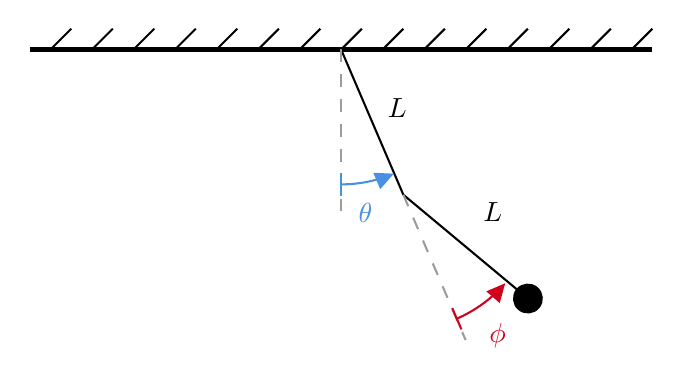
\begin{tikzpicture}[x=0.75pt,y=0.75pt,yscale=-1,xscale=1]
%uncomment if require: \path (0,300); %set diagram left start at 0, and has height of 300

%Straight Lines [id:da88879495030041] 
\draw [line width=1.5]    (480,80) -- (180,80) ;
%Straight Lines [id:da8592675948010826] 
\draw    (480,70) -- (470,80) ;
%Straight Lines [id:da3909809682368328] 
\draw    (460,70) -- (450,80) ;
%Straight Lines [id:da5390474411922489] 
\draw    (440,70) -- (430,80) ;
%Straight Lines [id:da0997286622802952] 
\draw    (420,70) -- (410,80) ;
%Straight Lines [id:da7214366710106086] 
\draw    (400,70) -- (390,80) ;
%Straight Lines [id:da5228157742795766] 
\draw    (380,70) -- (370,80) ;
%Straight Lines [id:da3575127382469875] 
\draw    (360,70) -- (350,80) ;
%Straight Lines [id:da4822573164742765] 
\draw    (340,70) -- (330,80) ;
%Straight Lines [id:da910185342676816] 
\draw    (320,70) -- (310,80) ;
%Straight Lines [id:da8454826691956545] 
\draw    (300,70) -- (290,80) ;
%Straight Lines [id:da9491977902298143] 
\draw    (280,70) -- (270,80) ;
%Straight Lines [id:da28933539575593303] 
\draw    (260,70) -- (250,80) ;
%Straight Lines [id:da5230450852671863] 
\draw    (240,70) -- (230,80) ;
%Straight Lines [id:da9457720673849641] 
\draw    (220,70) -- (210,80) ;
%Straight Lines [id:da10165059225338346] 
\draw    (200,70) -- (190,80) ;
%Straight Lines [id:da8370629677522231] 
\draw    (330,80) -- (360,150) ;
%Straight Lines [id:da40863186306124] 
\draw    (360,150) -- (420,200) ;
\draw [shift={(420,200)}, rotate = 39.81] [color={rgb, 255:red, 0; green, 0; blue, 0 }  ][fill={rgb, 255:red, 0; green, 0; blue, 0 }  ][line width=0.75]      (0, 0) circle [x radius= 6.7, y radius= 6.7]   ;
%Straight Lines [id:da04311473222375517] 
\draw [color={rgb, 255:red, 155; green, 155; blue, 155 }  ,draw opacity=1 ] [dash pattern={on 4.5pt off 4.5pt}]  (330,80) -- (330,160) ;
%Straight Lines [id:da1285462775825963] 
\draw [color={rgb, 255:red, 155; green, 155; blue, 155 }  ,draw opacity=1 ] [dash pattern={on 4.5pt off 4.5pt}]  (360,150) -- (390,220) ;
%Shape: Arc [id:dp034239614321454614] 
\draw  [draw opacity=0][line width=0.75]  (355.4,139.85) .. controls (347.6,143.17) and (339.01,145) .. (330,145) -- (330,80) -- cycle ; \draw [color={rgb, 255:red, 74; green, 144; blue, 226 }  ,draw opacity=1 ][line width=0.75]    (352.56,140.98) .. controls (345.53,143.58) and (337.93,145) .. (330,145) ; \draw [shift={(330,145)}, rotate = 360] [color={rgb, 255:red, 74; green, 144; blue, 226 }  ,draw opacity=1 ][line width=0.75]    (0,5.59) -- (0,-5.59)   ; \draw [shift={(355.4,139.85)}, rotate = 156.97] [fill={rgb, 255:red, 74; green, 144; blue, 226 }  ,fill opacity=1 ][line width=0.08]  [draw opacity=0] (8.93,-4.29) -- (0,0) -- (8.93,4.29) -- cycle    ;
%Shape: Arc [id:dp05018931071899502] 
\draw  [draw opacity=0][line width=0.75]  (409.06,192.64) .. controls (402.71,199.94) and (394.75,205.81) .. (385.75,209.7) -- (360,150) -- cycle ; \draw [color={rgb, 255:red, 208; green, 2; blue, 27 }  ,draw opacity=1 ][line width=0.75]    (407,194.9) .. controls (401.03,201.15) and (393.81,206.22) .. (385.75,209.7) ; \draw [shift={(385.75,209.7)}, rotate = 336.64] [color={rgb, 255:red, 208; green, 2; blue, 27 }  ,draw opacity=1 ][line width=0.75]    (0,5.59) -- (0,-5.59)   ; \draw [shift={(409.06,192.64)}, rotate = 131.02] [fill={rgb, 255:red, 208; green, 2; blue, 27 }  ,fill opacity=1 ][line width=0.08]  [draw opacity=0] (8.93,-4.29) -- (0,0) -- (8.93,4.29) -- cycle    ;

% Text Node
\draw (351,102.4) node [anchor=north west][inner sep=0.75pt]    {$L$};
% Text Node
\draw (397,152.4) node [anchor=north west][inner sep=0.75pt]    {$L$};
% Text Node
\draw (337,152.4) node [anchor=north west][inner sep=0.75pt]  [color={rgb, 255:red, 74; green, 144; blue, 226 }  ,opacity=1 ]  {$\theta $};
% Text Node
\draw (400,210.4) node [anchor=north west][inner sep=0.75pt]  [color={rgb, 255:red, 208; green, 2; blue, 27 }  ,opacity=1 ]  {$\phi $};

\end{tikzpicture}

    \caption{Double Pendulum Set-Up}
    \label{fig:Double Pendulum}
\end{figure}

\end{enumerate}


\newpage
\printendnotes

\chapter{Hamiltonian Mechanics}\label{chap:hamiltonian}

% maybe reduce the length of this, the Hamiltonian isn't actually that important for pure calculation, more for representation

After the formulation of \gls{Lagrangian} Mechanics, another formulation was created by Hamilton. The \gls{Hamiltonian} formulation, like the \gls{Lagrangian}, does not introduce any `new' concepts, because it is simply an alternate approach to dynamics. In fact, most of the time we have to find the \gls{Lagrangian} to construct our \gls{Hamiltonian}! So, the \gls{Hamiltonian}, does not even make most problems simpler to solve. Why is it important, then?

The first useful feature of the \gls{Hamiltonian} lies in the fact that it gives us a more intuitive feel for the system. The \gls{Lagrangian} has no physical meaning associated with it. $T-V$ doesn't describe any of attributes of the system we can point to and see. It is purely analytical. We \textit{need} the \gls{Lagrangian} to be $T-V$ for the formalism to work; there is no fundamental reason.

The \gls{Hamiltonian}, on the other hand, is often constructed as $H=T+V$. This is something we can recognize! It's the total energy of the system. So we can get a more intuitive feel for the system using the Hamiltonian. We know that energy is conserved in a conservative system, so it's simply changing form and that attribute allows us to understand the trajectory of the system. Something about that description sounds a bit more `fundamental than the \gls{Lagrangian}.

Secondly, and more important for our applications, is that the \gls{Hamiltonian} finds extensive use in the domain of optimal control! Here, we will outline the basics of \gls{Hamiltonian} mechanics and the relationship to optimal control will be explored in \autoref{part:control theory}.

Additionally, there is a nice geometrical interpretation that the \gls{Hamiltonian} can give us. We will give into the geometric interpretations later, and dive into them especially deep when we discuss symplectic manifolds and structure later. A good preview of the content to come in this chapter can be found in the wonderful article \cite{hirvonen_hamiltonian_nodate}.

\section{Derivation of the Hamiltonian}

After doing a few problems with the \gls{Lagrangian} approach to mechanics, we notice that the $\frac{d}{dt}\left(\frac{\partial L}{\partial \dot{q}_i}\right)$ term results in a second order derivative. If we want to solve this differential equation, then, we need to describe both the $q_i$'s and the $\dot{q}_i$'s. The effective analogy is that we need to know the initial position and velocity in order to integrate our acceleration \gls{eom}. So together, we have $2n$ independent variables that describe the full system motion.

What if we could transform one of these coordinates so that we instead have only first order derivatives? Luckily, we can do this! We'll use something called the \textit{Legendre Transform} to do so.

\subsection{The Legendre Transform}
The Legendre transform is the key mathematical tool that we will need in order to derive the \gls{Hamiltonian}. The Legendre transform is conceptually very simple -- it simply changes the variables we are using the our equation while still maintaining equivalence.

The way the Legendre transform accomplishes this is actually quite simple. There are geometric interpretations, but personally I feel that these geometric interpretations are more confusing than helpful.

It turns out that derivative of a function encodes a lot of information about the function! In fact, given just the derivative of a function, we can fully reconstruct the original function through integration. In fact, this is exactly what we do with numerical integration schemes, which you may read more about in Volume I. The only thing we are missing is some initial condition!

This is the key understanding that we need for the Legendre transform. We have some original function $f$ -- which in our case will be the \gls{Lagrangian} -- which we can transform by considering its derivative as the new input:
$$f\Rightarrow f^*\left(\frac{df}{dx}\right)$$
Of course, we also need to describe the initial condition. The Legendre transform does this for every point, by considering where the tangent line, with slope $\frac{df}{dx}$, intersects the origin. This guarantees that every single point has both a defined slope, as well as a defined starting point. To encode the origin intersection point, we take this to be the output of function $f^*$, so that 
$$f^*\left(\frac{df}{dx}\right)=-b$$
Where $b$ is the $y$-intercept we are intimately familiar with from algebra. Of course, we want to express $-b$ in terms of $\frac{df}{dx}$, that's what makes a functional expression useful! Here is where a geometric construction may help us. This is shown in \autoref{fig:Legendre}.

\begin{figure}[ht]
    \centering


\tikzset{every picture/.style={line width=0.75pt}} %set default line width to 0.75pt        

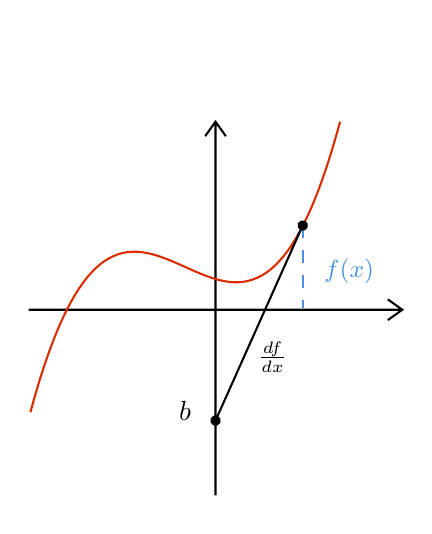
\begin{tikzpicture}[x=0.75pt,y=0.75pt,yscale=-1,xscale=1]
%uncomment if require: \path (0,300); %set diagram left start at 0, and has height of 300

%Straight Lines [id:da01484601527940943] 
\draw [color={rgb, 255:red, 74; green, 144; blue, 226 }  ,draw opacity=1 ] [dash pattern={on 4.5pt off 4.5pt}]  (302,90) -- (302,130) ;
%Shape: Axis 2D [id:dp9936162466939741] 
\draw  (170,130.59) -- (350,130.59)(259.99,40) -- (259.99,220) (343,125.59) -- (350,130.59) -- (343,135.59) (254.99,47) -- (259.99,40) -- (264.99,47)  ;
%Shape: Polynomial [id:dp0478973045554304] 
\draw  [color={rgb, 255:red, 218; green, 44; blue, 0 }  ,draw opacity=1 ] (170.81,180) .. controls (220.54,-4.8) and (270.27,224.8) .. (320,40) ;
%Straight Lines [id:da9433398230086687] 
\draw    (260,184) -- (302,90) ;
\draw [shift={(302,90)}, rotate = 294.08] [color={rgb, 255:red, 0; green, 0; blue, 0 }  ][fill={rgb, 255:red, 0; green, 0; blue, 0 }  ][line width=0.75]      (0, 0) circle [x radius= 2.01, y radius= 2.01]   ;
\draw [shift={(260,184)}, rotate = 294.08] [color={rgb, 255:red, 0; green, 0; blue, 0 }  ][fill={rgb, 255:red, 0; green, 0; blue, 0 }  ][line width=0.75]      (0, 0) circle [x radius= 2.01, y radius= 2.01]   ;

% Text Node
\draw (241,173.4) node [anchor=north west][inner sep=0.75pt]    {$b$};
% Text Node
\draw (311,104.4) node [anchor=north west][inner sep=0.75pt]  [font=\small,color={rgb, 255:red, 74; green, 144; blue, 226 }  ,opacity=1 ]  {$f( x)$};
% Text Node
\draw (279,144.4) node [anchor=north west][inner sep=0.75pt]  [font=\small,color={rgb, 255:red, 0; green, 0; blue, 0 }  ,opacity=1 ]  {$\frac{df}{dx}$};


\end{tikzpicture}
    \caption{Geometric construction of Legendre Transform}
    \label{fig:Legendre}
\end{figure}
We can see that taking $\frac{df}{dx}$ and multiplying by the distance $x$, we get from point $b$ to $f(x)$. We can represent this as $\frac{df}{dx}x=f(x)-b$.

We know that $f^*\left(\frac{df}{dx}\right)=-b$, so we can rearrange to solve for this in the equation above to get:
\begin{gather}\label{eq:legendre}
    \color{blue}\boxed{\color{black}f^*\left(\frac{df}{dx}\right)=\frac{df}{dx}x-f(x)}\\
    \color{blue}\mathrm{Legendre \ Transform}
\end{gather}
\section{What is Momentum?}
Now that we are equipped with the Legendre transform, we are ready to tackle the \gls{Hamiltonian}. To do so, we will need to define a new quantity, the momentum.

Of course, many of us are familiar with the concept of momentum from introductory physics classes, or even higher level classes. Typically, we define the momentum to be $mv$. However, this concept only entails linear momentum! We also have angular momentum, $r\times mv$.

\newglossaryentry{gen momentum}
{
    name=generalized momentum,
    first = {\textit{generalized momentum}},
    plural = {generalized momenta},
    description={A generalized coordinate that is defined as $\frac{\partial L}{\partial \dot{q}_i}.$ Generalized momentum is mostly used in Hamiltonian mechanics}
}

Furthermore, if you are familiar with quantum mechanics, you likely know that momentum can also be represented as $-i\hbar\frac{\partial}{\partial x}$. We know that the momentum of a relativistic particle is also different, given by $\gamma m_0v$. You may have also heard that photons have momentum. It seems that our notion of momentum of $mv$ is in dire need of a new, more general formulation! Of course, it is okay if you've never seen these representations of momentum before. They are here simply to show that momentum is a concept that is very broad. 

What we hope to accomplish is to capture all of these in a single formula for momentum. As a result, we should define a \textit{generalized momentum}, analogous to what we have done for generalized positions and velocities. 

Of course, this notion of the \gls{gen momentum} is more flexible than the ordinary momentum. To define the \gls{gen momentum}, we can consider the example of a free particle -- that is a particle acted upon by no potentials or forces.

\begin{example}[The Free Particle]
    The free particle has one of the simplest possible \glspl{Lagrangian}. Since there are no potentials involved, we can fully describe the \gls{Lagrangian} of the free particle with $L=T$. Since the object is a point mass particle, the \gls{Lagrangian} is thus $$L=\frac{1}{2}m\dot{x}^2$$
We can use the Euler-Lagrange equation here to find the equation of motion quite easily. The first term, $\frac{\partial L}{\partial x}$ goes to zero since there is no dependence on $x$. This leaves only the $\frac{d}{dt}\frac{\partial L}{\partial \dot{x}}=0$ term, which must be a constant. Upon evaluation, we have $m\dot{x}=C$, which means that the linear momentum, $m\dot{x}$ is conserved because it is constant! Moreover, it seems we have found a way to get the momentum from the \gls{Lagrangian}!
\end{example}

As it turns out, the way that we calculated the momentum in the example, as $\frac{\partial L}{\partial \dot{x}}$, is the way that we find the \gls{gen momentum}. We can formalize this for any generalized velocity, as
\begin{gather}
    \color{blue}\boxed{\color{black}p_j=\frac{\partial L}{\partial\dot{q}_j}}\\
    \color{blue}\mathrm{Generalized\ Momentum}
\end{gather}
This definition of \gls{gen momentum} is much more powerful than the standard definition that we use. This definition, in fact, solves all of the problems that we listed before. By using the definition with the \gls{Lagrangian}, we are able to solve problems in quantum mechanics, special relativity, and of course, classical mechanics!

Additionally, we can see the presence of a derivative in this definition goes hand in hand with the previously discussed Legendre transform.
\subsection{From the Lagrangian to the Hamiltonian}
With the \gls{gen momentum} defined, we are now ready to describe the \gls{Hamiltonian} in full. We will start with the \gls{Lagrangian}, which we can describe very broadly as a function of $q$ and $\dot{q}$:
$$L(q_j,\dot{q}_j)$$
Using the Legendre transform, we can transform $\dot{q}$ into a new variable. We replace $f$ with $L$ and $x$ with $\dot{q}$ in \eqautoref{eq:legendre} to get the following:
$$L^*\left(\frac{\partial L}{\partial \dot{q}_j}\right)=\frac{\partial L}{\partial \dot{q}_j}\dot{q}_j-L$$
We can recognize that the term $\frac{\partial L}{\partial \dot{q}}$ is the \gls{gen momentum} that we have just described! We can simplify the equation by calling this term $p$. We will also denote $L^*$ as $\mathcal{H}$:
$$\mathcal{H}(q_j,p_j)=p_j\dot{q}_j-L$$
We can notice that the expression for the \gls{Hamiltonian} still has $\dot{q}_j$ in it, so we still need an expression for the generalized velocities. However, we no longer need to take the derivative with respect to this term, so we have reduced the order of the differential equation. By the garuntees of the Legendre transformation, we have also made sure that all of the relevant information in the system is still there!

\section{The Hamiltonian as Total Energy}
In the introduction to this section, I mentioned that the \gls{Hamiltonian} has an interpretation as the total energy of the system. We can showcase this with the familiar example of the free particle:

\begin{example}[Hamiltonian of free particle]
    As before, we will consider a free particle subject to no external forces or potentials. We can utilize the \gls{Lagrangian} which we have previously found:
    $$L=\frac{1}{2}m\dot{x}^2$$
    Additionally, we know the generalized momentum of the particle to be:
    $$\frac{\partial L}{\partial \dot{x}}=p=m\dot{x}$$
    Which is equivalent to the standard definition of linear momentum in this case. We can, in fact, check that linear momentum is conserved in the system by noting that $x$ is a cyclic coordinate and has 
\end{example}

Let u

\section{Hamilton's Equations of Motion}
When we create a \gls{Lagrangian}, we can apply the Euler-Lagrange equations to derive \glspl{eom}. In the case of \gls{Hamiltonian} mechanics, we can derive a similar relationship for the equations of motion. The same machinery of the calculus of variations can be used to derive these relationships.

Using relations with the \gls{Lagrangian}, we can write two first order differential equations for the \gls{eom} with the \gls{Hamiltonian}.

\begin{gather}
\color{blue}\boxed{
\begin{array}{c}\color{black}
     \dot{q}_j=\dfrac{\partial \mathcal{H}}{\partial p_j}\\\\
     \color{black}
  -\dot{p}_j=\dfrac{\partial \mathcal{H}}{\partial q_j}
\end{array}
}\\
\color{blue}\mathrm{Hamiltonian \ EOM's}
\end{gather}



\section{An Analogy With Fluid Dynamics}
Many aerospace and mechanical engineers have seen fluid dynamics and studied it fairly extensively. As it turns out, there is a beautiful relationship between \gls{Hamiltonian} systems and a fluid dynamics analogy which will be explored in this section.



\section{Ostrogradsky instability}
Why natural phenomenon are typically of 2nd order

not writing any more rn because I don't know it

This shit too complicated probably



\chapter{Introductory Astrodynamics}
If we loosen our definition of rocket modeling \textit{slightly}, orbital mechanics becomes a very important part of our discussion. The \gls{Lagrangian} and \gls{Hamiltonian} description of mechanics are instrumental to orbital applications. Because many of the applications of our previously mentioned dynamics are in the realm of spacecraft dynamics, I feel it is a necessity to include information on orbits. 

Additionally, we will find that energy mechanics has extensive uses here, as space is the perfect playground for our 'no frictional forces or drag' that we often use for energy mechanics. This chapter will essentially be an extension of the discussion of spacecraft in Volume II, with a specific focus placed on spacecraft applications. Of course, to anyone who has played Kerbal Space Program, some parts of this section may feel quite familiar. We will solidify that intuition with the mathematical tools needed in our engineering systems.

\section{Orbital Mechanics Introduction}
There is no better place to start with orbital mechanics than the humble 2-D conic orbit. These orbits are simple to describe and derive from elementary physics, but are extraordinarily powerful. We will keep utilizing these orbits far into our study of orbital mechanics!

\section{2-D Conic Orbits}
2-D Conic orbits are the simplest orbits that we can describe which model the physical behaviors of a gravitational system. In a conic orbit, we consider only a single force acting on the body, gravity. We express this force with Newton's famous law of Universal Gravitation:
$$\ddot{r}=-\frac{GM}{r^2}\hat{e}_r$$
There are many sources which proceed to compute many equations of orbital mechanics using Newtonian mechanics and other laws, such as the fact that angular momentum must be conserved. Most of these approaches end up using energy relations at some point during their derivation, so we may as well start there!

\subsection{The Lagrangian Approach}

Because these Newtonian derivations are abundant, I will instead proceed from the \gls{Lagrangian} point of view, which will give us many insights, and all of the results will come directly from the mathematical architecture.

We know that gravitational forces are a conservative force. That is -- the change in energy is only dependent on the distance from the gravitational field. This makes the \gls{Lagrangian} description very convenient. As is typical, we define the \gls{Lagrangian} of the system to be $L=T-V$.

In a two dimensional orbit, there are two ways we can move: tangentially or radially. In the tangential direction, this velocity is simply $\dot{r}\hat{e}_r$. In the radial direction, this velocity is $r\dot{\theta
}\hat{e}_{\theta}$. Thus, the total velocity is simply the addition of these two orthogonal components:
$\vec{v}=\dot{r}\hat{e}_r+r\dot{\theta}\hat{e}_\theta$ (you can easily show this with use of the \gls{bke}). From here it is trivial to find the specific kinetic energy, $\frac{1}{2}\vec{v}^2$.

We can describe the potential as a function of the radius only. Since the potential is conservative, it is known that $F=-\nabla U$ (The force derives from a potential, as a physicist may say). We can of course reverse this statement to find an expression for $U$.

This equation reduces quite readily in this scenario. Since the force is only a function of the radial component, we have reduced the equation to $$F(r)=-\frac{\partial U}{\partial r}$$
This can easily be integrated to attain an expression for $U$. We first fully expand $F(r)$ and isolate $\partial U$:
$$-\frac{GM}{r^2}\partial r=-\partial U$$
Since both sides are single-variate, the partial derivatives reduce to ordinary total derivative. We then integrate to attain the following:
$$\int\frac{GM}{r^2} dr=\int dU$$
Upon evaluation, we have the following:
$$\frac{-GM}{r}=U+C$$
It is customary to assume that the potential goes to zero at an infinite distance. We can apply this condition to find that $C=0$, which leaves us with the gravitational potential:
$$U(r)=\frac{-GM}{r}$$
We now have all of the components necessary to construct our \gls{Lagrangian}, which gives us
$$L=\frac{1}{2}\left[\dot{r}^2+\left(r\dot{\theta}\right)^2\right]+\frac{GM}{r}$$
Now we can start evaluating the \gls{Lagrangian} to find the equations of motion!

We start with the equation for $\theta$, which gives us:
$$\frac{\partial L}{\partial \theta}-\frac{d}{dt}\frac{\partial L}{\partial \dot{\theta}}=0$$
We notice that no terms contain $\theta$, so our \gls{eom} for this direction reduces to
$$\frac{d}{dt}\frac{\partial L}{\partial \dot{\theta}}=0$$
We can remove all the $\dot{r}^2$ and $\frac{GM}{r}$ terms via the linearity of the derivative since these have no dependence on $\dot{\theta}$. This leaves us with the following upon evaluation of the partial derivative:
$$\frac{d}{dt}\left(r^2\dot{\theta}\right)=0$$
Since this derivative is zero, $r^2\dot{\theta}$ must be a constant. This $r^2\dot{\theta}$ is in fact our (specific) angular momentum, $r\times v$! So we have recovered fully mathematically that the angular momentum of the orbit must be conserved. We will define this specific angular momentum $h$.

Let us then move on to the second equation, which is 
$$\frac{\partial L}{\partial r}-\frac{d}{dt}\frac{\partial L}{\partial \dot{r}}=0$$
This requires a bit more computation, but is still straightforward. We can proceed with the computation to get
$$\ddot{r}=r\dot{\theta}^2-\frac{GM}{r^2}$$
This is the equation of motion for the orbit! From here, we can numerically integrate this equation to get any orbit we want. However, this is a case where we can find an exact analytic solution.

\subsection{The Analytical Solution of the Orbit}
Central force problem Goldstein

\section{3-D Conic Orbits}
\subsection{The Euler Angles}

\section{Orbit Transfers}

\section{Numerical Simulation of Orbits}
\subsection{Basic N-Body simulations}
\subsection{CR3BP}
\subsection{Lambert Equation}
\subsection{Trajectory Optimization}
\subsection{Gravity Assists and Multiple Transfers}